\documentclass[a4paper,fleqn]{cas-sc}

\usepackage[authoryear]{natbib}

\usepackage{enumitem}
\usepackage{tikz, pgfplots, pgf-pie, longtable, tabularx, makecell}
\pgfplotsset{compat=1.18}

\usetikzlibrary{shapes,arrows,positioning,chains}


\begin{document}

\let\WriteBookmarks\relax
\def\floatpagepagefraction{1}
\def\textpagefraction{.001}

\shorttitle{Gamification of history education: a systematic review}

\title[mode=title]{Gamification of history education: a systematic review}

%\shortauthors{S. S. Korniienko and S. O. Semerikov}
%
%\author[1]{Serhii S. Korniienko}[%
%orcid={0000-0002-2573-2115},
%]
%\ead{korniienko.serhii@kdpu.edu.ua}
%
%\credit{Data curation, Formal analysis, Investigation, Software, Visualization, Writing -- Original Draft, Writing -- Review \& Editing}
%
%
%
%\author[1,2,3,4]{Serhiy O. Semerikov\corref{cor1}}[
%orcid=0000-0003-0789-0272,
%]
%\ead{semerikov@gmail.com}
%\ead[url]{https://acnsci.org/semerikov}
%
%\credit{Conceptualization, Methodology, Resources, Software, Supervision, Validation, Visualization, Writing -- Original Draft, Writing -- Review \& Editing}
%
%\cortext[cor1]{Corresponding author}
%
%\affiliation[1]{organization={Kryvyi Rih State Pedagogical University},
%	addressline={54~Universytetskyi~Ave.},
%	city={Kryvyi~Rih},
%	postcode={50086},
%	%	state={},
%	country={Ukraine}}
%
%\affiliation[2]{organization={Institute for Digitalisation of Education of the NAES of Ukraine},
%	addressline={9~M.~Berlynskoho~Str.},
%	city={Kyiv},
%	postcode={04060},
%	%	state={},
%	country={Ukraine}}
%
%\affiliation[3]{organization={Zhytomyr Polytechnic State University},
%	addressline={103 Chudnivsyka Str.},
%	city={Zhytomyr},
%	postcode={10005},
%	%	state={},
%	country={Ukraine}}
%
%\affiliation[4]{organization={Academy of Cognitive and Natural Sciences},
%	addressline={54~Universytetsky~Ave.},
%	city={Kryvyi~Rih},
%	postcode={50086},
%	%	state={},
%	country={Ukraine}}
%
%
%\begin{abstract}
%	Gamification has emerged as a promising pedagogical approach for history education, yet the evidence base remains fragmented across diverse definitions and contexts. This systematic review synthesises empirical and design-based studies published between 2000 and 2024 to examine how gamification is conceptualised, its effectiveness, design principles, and implementation challenges. From an initial pool of 4,011 records, 74 studies meeting eligibility criteria were analysed using a narrative synthesis. Results indicate that while 85.1\% of studies lacked an explicit definition of gamification, the majority reported positive effects on historical knowledge acquisition and student engagement. Common design elements included exploration mechanics, narrative storytelling, and collaborative structures. However, the review identified substantial methodological limitations: 83.8\% of studies exhibited a high risk of bias, frequently characterised by small sample sizes, absent control groups, short interventions, and reliance on self-reported outcomes. Implementation barriers included technical constraints, resource limitations, and curriculum integration difficulties. The study concludes that while gamification shows potential for enhancing history education, the current body of literature lacks robust causal evidence. Future research must prioritise rigorous experimental designs with larger samples, longitudinal timeframes, and standardised instruments to validate these pedagogical benefits.
%\end{abstract}

\begin{highlights}
	\item Systematic review synthesises 74 studies on gamification in history education.
	\item Interventions predominantly enhanced student engagement and knowledge acquisition.
	\item 85.1\% of studies lacked an explicit definition of gamification concepts.
	\item High risk of bias and small sample sizes characterise the current evidence base.
	\item Future research requires longitudinal designs and rigorous control groups.
\end{highlights}
	

%\begin{keywords}
%	gamification \sep history education \sep systematic review
%\end{keywords}

\maketitle

%\section{Introduction}
%
%The rapid digital transformation of education in the 21st century has led to a significant shift in the symbols associated with learning. Whereas books, globes, and pencils were once the primary emblems of education \citep{symbolismhub.com}, today, smartphones have become the dominant representation \citep[p.~15]{UNESCO2023}. This shift reflects not only the increasing integration of technology in classrooms but also the evolving needs and preferences of learners in the digital age.
%
%However, the proliferation of digital tools and resources has also brought forth new challenges, such as information overload, which can adversely affect learners' mental health and well-being \cite[p.~83]{UNESCO2023}. To address these concerns and engage students effectively, educators are exploring innovative pedagogical approaches that leverage the affordances of digital technologies. One such approach that has gained significant attention in recent years is gamification -- the incorporation of game design elements in non-game contexts, such as education \citep{Deterding2011}.
%
%Gamification has the potential to transform learning experiences by making them more engaging, motivating, and enjoyable for students. By tapping into the inherent human desire for competition, achievement, and rewards, gamified learning environments can foster greater student participation, persistence, and knowledge retention \citep{Sailer2017}. Moreover, gamification can promote the development of essential 21st-century skills, such as problem-solving, collaboration, and creativity \citep{Qian2016}.
%
%However, implementing gamification in education is not without its challenges. Designing effective gamified learning experiences requires careful planning, pedagogical expertise, and an understanding of game design principles \citep[p.~77]{UNESCO2023}. Additionally, there is a risk that students and teachers may perceive gamification as merely an entertainment tool rather than a purposeful educational strategy. Therefore, it is crucial to examine the existing research on gamification in education to identify best practices, potential pitfalls, and areas for future investigation.
%
%
%This systematic review aims to synthesize the current state of knowledge on gamification in education, with a specific focus on its application in the field of history education. 
%By critically analyzing and integrating findings from diverse empirical studies, this review seeks to provide a comprehensive understanding of how gamification is conceptualized, implemented, and evaluated in educational contexts. The following research questions will guide this review:
%\begin{enumerate}[label=RQ\arabic*:,leftmargin=*,noitemsep]
%\item How is gamification defined and conceptualized in the context of education, particularly in history education?
%\item What is the current state of research on the effectiveness of gamification in enhancing learning outcomes and student engagement in history education?
%\item What are the key design principles, strategies, and technologies used in implementing gamification in history education?
%\item What are the main challenges, limitations, and potential negative effects associated with gamification in history education?
%\end{enumerate}
%
%While the review by \citet{Oceja2022419} provides valuable insights into the use of games for teaching history and geography in secondary education, an updated review is still necessary for several reasons:
%\begin{enumerate}[noitemsep]
% \item 
%\textit{Scope and focus}: the \citet{Oceja2022419} review focused specifically on secondary education and included both history and geography, while this review has a different scope, focusing solely on history education and including all educational levels (primary, secondary, and tertiary education).
%
% \item 
%\textit{Methodology and inclusion criteria}: this review employed different sources and inclusion criteria, which could lead to the identification of additional relevant studies not covered by \citet{Oceja2022419}.
%
% \item 
%\textit{Conceptualization and definition}: this review aims to examine how gamification is defined and conceptualized in the context of history education (RQ1), an aspect not explicitly addressed by \citet{Oceja2022419}.
%
% \item 
%\textit{Effectiveness and learning outcomes}: this review places a strong emphasis on evaluating the effectiveness of gamification in enhancing learning outcomes and student engagement (RQ2), whereas \citet{Oceja2022419} only briefly touched on the measurement of educational impact for a subset of studies using commercial off-the-shelf games (RQ4).
%
% \item 
%\textit{Design principles, strategies, and technologies}: this review seeks to identify the key design principles, strategies, and technologies used in implementing gamification in history education (RQ3), an aspect not directly addressed by \citet{Oceja2022419}, who focused more on the types of games and methodological approaches used (RQ2 and RQ3).
%
% \item 
%\textit{Challenges, limitations, and negative effects}: this review aims to provide a comprehensive understanding of the main challenges, limitations, and potential negative effects associated with gamification in history education (RQ4), an important consideration for educators and researchers not covered in the \citet{Oceja2022419} review.
%
%\end{enumerate}
%
%The remainder of this article is structured as follows. Section \ref{sec:Methodology} outlines the methodology used to systematically search, screen, and synthesize the existing literature on gamification in history education. Section \ref{sec:Results} presents the results, addressing each of the four research questions. Section \ref{sec:Discussion} discusses the implications of the findings, highlights gaps and limitations, and provides recommendations for future research and practice. Finally, Section \ref{sec:Conclusion} summarizes the key conclusions.
%
%
%% \section{Literature review}
%
%
%\section{Methods}
%\label{sec:Methodology}
%% ## Methods
%% Provide more details in your methodology section:
%% - All databases, registers, websites searched with dates 
%% - Full search strategies used, including limits and filters
%% - Processes for selecting studies, including automation tools used
%% - Methods for data extraction, including how many reviewers extracted data
%% - List of excluded studies with justification for exclusions
%
%\subsection{Protocol and registration}
%
%This systematic review adheres to the Preferred Reporting Items for Systematic Reviews and Meta-Analyses (PRISMA) 2020 statement \citep{Page2021}. While no formal protocol was registered in a public repository such as PROSPERO, the review methodology was established a priori, with eligibility criteria, search strategy, and data extraction procedures determined before database searching commenced. This approach ensures methodological transparency while acknowledging the exploratory nature of this initial systematic synthesis in digital history pedagogy.
%
%\subsection{Eligibility criteria}
%% The criteria for including articles are outlined by scientometric databases (Scopus, Web of Science, Dimensions), and language of publication (English, Ukrainian) and type (- - - - - - -).
%The following eligibility criteria were applied to select studies for inclusion in this systematic review:
%
%\begin{itemize}[noitemsep]
% \item \textit{Population}: studies involving students in primary, secondary, or higher education settings who are learning history.
% \item \textit{Intervention}: studies that investigate the use of gamification techniques, elements, or strategies in history education. Gamification refers to the application of game design elements in non-game contexts.
% \item \textit{Comparator}: studies comparing gamification interventions to traditional teaching methods, other educational interventions, or no intervention.
% \item \textit{Outcomes}: studies that measure learning outcomes (e.g., knowledge acquisition, retention, engagement, motivation, or attitudes) or student perceptions of the gamification intervention.
% \item \textit{Study designs}: empirical studies using quantitative, qualitative, or mixed methods, including experimental, quasi-experimental, and observational designs; literature reviews, conceptual papers, and opinion pieces were excluded.
% \item \textit{Setting}: studies conducted in formal educational settings (e.g., classrooms, online courses) or informal learning environments (e.g., museums, historical sites).
% \item \textit{Time frame}: studies published between 2000 and 2024, to capture the most recent developments in the field of gamification and history education.
% \item \textit{Publication status}: peer-reviewed journal articles, conference papers, and book chapters. Unpublished manuscripts, dissertations, and grey literature will be excluded.
% \item \textit{Language}: studies published in English or Ukrainian.
% \item \textit{Databases}: studies indexed in Scopus, Web of Science, or Dimensions databases.
%\end{itemize}
%
%Studies will be excluded if they do not meet the above criteria, if the full text is not available, or if they do not provide sufficient information to assess eligibility. In cases where multiple reports of the same study are identified, the most comprehensive or recent version will be included.
%%
%%
%%
%%
%%% Note: Exclusion criteria removed because they contradicted the inclusion criteria above
%%% (inclusion says ``primary, secondary, or higher education'' but exclusion said ``exclude K-12'').
%%% All exclusion logic is captured by the inclusion criteria: studies not meeting the above
%%% criteria were excluded.
%%
%%
%%
%%
%%
%%
%%
%\subsection{Information sources}
%
%% To identify studies the appeal to the bases was made on 01.07.2024.
%
%The following databases were searched to identify potentially eligible studies: Scopus \citep{scopus}, Web of Science \citep{wos}, and Dimensions \citep{dimensions}. All databases were searched from their inception to July 17, 2024. The search was limited to studies published in English or Ukrainian.
%
%The reference lists of included studies and relevant systematic reviews \citep{Oceja2022419} and others) were used while discussing the research results.
%
%
%\subsection{Search strategy}
%% According to the PRISMA protocol, after defining the data source, the search strategies was defined (i.e., the keywords used to assemble the search string). Te query/search string used was: TITLE-ABS-KEY (gamification) AND TITLE-ABS-KEY (game-based learning) OR TITLE-ABS-KEY (serious game) AND TITLE-ABS-KEY (history education) OR TITLE-ABS-KEY (teaching history) OR TITLE-ABS-KEY (history learning).
%
%
%The search strategy was based on the eligibility criteria and included a combination of keywords and subject headings related to gamification, game-based learning, serious games, and history education.
%
%The following limits specified in the eligibility criteria, were applied to the search strategy:
%
%\begin{itemize}[noitemsep]
% \item \textit{Time frame}: the search was limited to studies published between 2000 and 2024.
% 
% \item \textit{Language}: the search was limited to studies published in English or Ukrainian. 
% 
% \item \textit{Publication status}: the search was limited to peer-reviewed journal articles, conference papers, and book chapters.
%\end{itemize}
%
%No other limits were applied to the search strategy to ensure a comprehensive and unbiased search.
%
%The search strategy was adapted for each database, using appropriate syntax:
%
%\begin{itemize}[noitemsep]
% \item Advanced search query for Scopus database by paper titles:
%
%\begin{verbatim}
%TITLE ( 
% history 
% AND 
% ( 
% game* 
% OR 
% gamification 
% ) 
% AND 
% ( 
% education 
% OR 
% teaching 
% OR 
% learning 
% OR 
% student* 
% OR 
% instruction 
% ) 
%) 
%AND 
%(
% PUBYEAR > 1999 
% AND 
% PUBYEAR < 2025 
%) 
%AND 
%( 
% LIMIT-TO ( LANGUAGE , "English" ) 
% OR 
% LIMIT-TO ( LANGUAGE , "Ukrainian" ) 
%) 
%AND 
%( 
% LIMIT-TO ( DOCTYPE , "cp" ) 
% OR 
% LIMIT-TO ( DOCTYPE , "ar" ) 
% OR 
% LIMIT-TO ( DOCTYPE , "ch" ) 
%)
%\end{verbatim}
%
% \item Advanced search query for Web of Science Core Collection database (\url{https://www.webofscience.com/wos/woscc/summary/19e8ad4d-0dcf-493f-b0ee-56751bbadca2-fc405b9b/relevance/1}) by paper titles:
%
%\begin{verbatim}
%history AND (game* OR gamification) AND 
%(education OR teaching OR learning OR student* OR instruction) (Title) 
%and 2000-2024 (Year Published) 
%and English OR Ukrainian (Language) 
%and Article OR Book Chapter OR Proceedings Paper (Document Type)
%\end{verbatim}
%
% \item Basic search query for Dimensions database is shown in Figure~\ref{dimensions_query}.
%\end{itemize}
%
%\begin{figure}
% \centering
% 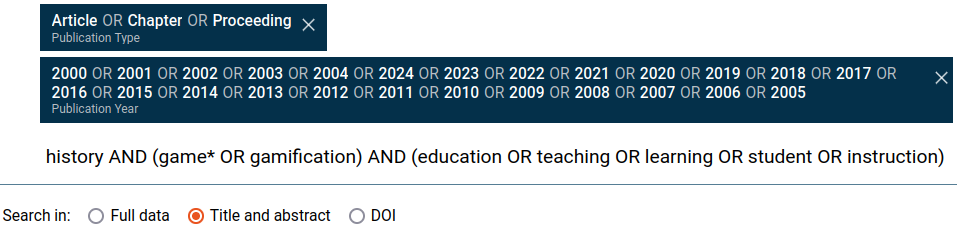
\includegraphics[width=\linewidth]{dimensions_query.png}
% \caption{Search query for Dimensions database.}
% \label{dimensions_query}
%\end{figure}
%
%For Scopus and Web of Science, all limits were satisfied, while for Dimensions, the papers were selected in any language, and the search keywords were applied to both the titles and abstracts.
%
%
%\subsection{Selection process}
%
%
%The process of selecting articles for review considered PRISMA guidelines \citep{Page2021} as shown in Figure~\ref{fig1}.
%
%
%\begin{figure}[ht!]
%\centering
%\begin{tikzpicture}[
%node distance = 8mm and 5mm,
%start chain = A going below,
%box/.style = {draw, 
%% minimum width=30mm, minimum height=10mm, 
%align=center},
%arrow/.style = {thick,-stealth}
%]
%
%\node [box, minimum width=44mm, minimum height=2.2cm] (records) {Records identified from\\
%Scopus (\textit{n} = 119);\\
%Web of Science \\Core Collection (\textit{n} = 78);\\
%Dimensions (\textit{n} = 3799)};
%
%\node [box, right=of records, minimum width=58mm, minimum height=2.2cm] (removed) {Records removed before screening:\\ 
%1) records from the Dimensions \\ marked as ineligible\\
%by automation tool (\textit{n} = 3776);\\
%2) duplicate records removed (\textit{n} = 69)};
%
%\node [box, below=of records, minimum width=44mm, minimum height=1.6cm] (screened) {Records screened\\(\textit{n} = 151)};
%
%\node [box, right=of screened, minimum width=58mm, minimum height=1.6cm] (excluded) {Records excluded by violation of:\\
%1) language criteria (\textit{n} = 3);\\
%2) population criteria (\textit{n} = 2)};
%
%\node [box, below=of screened, minimum width=44mm, minimum height=1cm] (sought) {Articles sought for retrieval:\\
%(\textit{n} = 146)};
%
%\node [box, right=of sought, minimum width=58mm, minimum height=1cm] (notret) {Articles not retrieved\\(\textit{n} = 25)};
%
%\node [box, below=of sought, minimum width=44mm, minimum height=2.2cm] (assessed) {Articles assessed \\for eligibility\\(\textit{n} = 121)};
%
%\node [box, right=of assessed, minimum width=58mm, minimum height=2.2cm] (exclude) {Articles excluded by violation of:\\ 1) one criterion (\textit{n} = 10);\\
% 2) two criteria (\textit{n} = 9);\\
% 3) three criteria (\textit{n} = 12);\\
% 4) four criteria (\textit{n} = 9)
%};
%
%\node [box, below=of assessed, minimum width=44mm, minimum height=1.6cm] (fulltext) {Articles assessed at\\full-text level\\(\textit{n} = 80)};
%
%\node [box, right=of fulltext, minimum width=58mm, minimum height=1.6cm] (excludefull) {Articles excluded during\\extraction (\textit{n} = 6):\\not history education (3);\\systematic review (1);\\history of mathematics (1);\\no gamification (1)};
%
%\node [box, below=of fulltext, minimum width=44mm, minimum height=1cm] (included) {Studies included in\\narrative synthesis\\(\textit{n} = 74)};
%
%\node [box, left=of records, align=center, minimum height=2.2cm, minimum width=5mm] (identification) {\rotatebox{90}{\textbf{Identification}}};
%\node [box, left=of included, align=center, minimum height=2.5cm, minimum width=5mm] (includedleft) {\rotatebox{90}{\textbf{Included}}};
%\node [box, left=of assessed, yshift=-0.3cm, minimum height=6.3cm, align=center, minimum width=5mm] (screening) {\rotatebox{90}{\textbf{Screening}}};
%
%
%\draw [arrow] (records) -- (removed);
%\draw [arrow] (records) -- (screened);
%\draw [arrow] (screened) -- (excluded);
%\draw [arrow] (screened) -- (sought);
%\draw [arrow] (sought) -- (notret);
%\draw [arrow] (sought) -- (assessed);
%\draw [arrow] (assessed) -- (exclude);
%\draw [arrow] (assessed) -- (fulltext);
%\draw [arrow] (fulltext) -- (excludefull);
%\draw [arrow] (fulltext) -- (included);
%
%\end{tikzpicture} 
%\caption{Flow diagram for the systematic review following the PRISMA statement.}
%\label{fig1}
%\end{figure}
%
%During the identification stage, 3776 records from the Dimensions database were removed because the paper titles did not contain needful keywords (history AND (game* OR gamification) AND (education OR teaching OR learning OR student* OR instruction)).
%%
%%
%%
%%
%%
%%
%
%Appendix~\ref{appA} contains the program code used to select records from the XLSX files exported from the Dimensions database by paper titles.
%%
%%
%%
%%
%%
%%
%We found 58 duplicate records in the Web of Science Core Collection, which were identified from the Scopus database, and 11 duplicate records in the Dimensions database, which were identified from the Scopus and/or Web of Science Core Collection databases.
%
%Among 12 unique records from the Dimensions database, 3 were presented in languages other than English and Ukrainian. 2 publications violated population criteria.
%
%In total, 25 articles were not retrieved. Therefore, 121 articles were assessed for eligibility.
%
%The preliminary automatic assessment was made using LLM Claude 3.5 Sonnet:
%
%\begin{verbatim}
%I would like to assess a set of papers on the following eligibility criteria:
%
%1. Language: paper published in English or Ukrainian.
%2. Publication status: peer-reviewed journal article, conference paper or book chapter. 
%3. Setting: the study was conducted in formal educational settings (e.g., classrooms, 
%online courses) or informal learning environments (e.g., museums, historical sites).
%4. Study designs: empirical studies using quantitative, qualitative, or mixed methods, 
%including experimental, quasi-experimental, and observational designs; literature reviews, 
%conceptual papers, and opinion pieces must be excluded.
%5. Outcomes: studies that measure learning outcomes (e.g., knowledge acquisition, 
%retention, engagement, motivation, or attitudes) or student perceptions of the 
%gamification intervention.
%6. Intervention: studies that investigate the use of gamification techniques, elements, or 
%strategies in history education.
%7. Population: studies involving students in primary, secondary, or higher education 
%settings who are learning history.
%
%The answer to every question should be 1 (yes) or 0 (no) without any comments. 
%Example of answer:
%1
%1
%0
%1
%1
%1
%1
%\end{verbatim}
%
%Two researchers then independently reviewed the assessment results provided by Claude 3.5 Sonnet. They checked each article to ensure it met the inclusion criteria. Any disagreements were resolved through discussion until a consensus was reached.
%
%4 articles marked by LLM as suspicious have been included after manual review. During the manual review, 1 article was excluded because it was related to the patient's medical history. 40 articles were excluded by violation of at least one eligibility criterion:
%
%\begin{itemize}[noitemsep]
% % one criterion -- 10
% % two criteria -- 9
% % three criteria -- 12
% % four criteria -- 9
% \item study designs -- 6 article;
% \item intervention -- 2 articles;
% \item outcomes -- 1 article;
% \item population -- 1 article;
%
% \item study designs, and outcomes -- 5 articles;
% \item study designs, and population -- 2 articles;
% \item intervention, and population -- 2 articles;
%
% \item study designs, outcomes, and population -- 6 articles;
% \item setting, study designs, and outcomes -- 3 articles;
% \item study designs, outcomes, and intervention -- 2 articles;
% \item setting, intervention, and population -- 1 article;
%
% \item study designs, outcomes, intervention, and population -- 4 articles;
% \item setting, study designs, outcomes, intervention, and population -- 3 articles;
% \item setting, study designs, outcomes, and population -- 1 article;
% \item setting, study designs, outcomes, and intervention -- 1 article;
%\end{itemize}
%
%
%In total, 41 articles were excluded during the manual review process, leaving 80 articles for full-text assessment. Of these, 6 were subsequently excluded during detailed data extraction (3 not about history education, 1 systematic review, 1 about history of mathematics, 1 without gamification), yielding 74 studies included in the narrative synthesis. The reasons for exclusion were documented in the spreadsheet.
%
%% The multi-step selection process, involving both automated assessment by Claude and manual review by two researchers, helped ensure the rigour and reliability of the article selection.
%
%
%\subsection{Data collection process}
%For each of the 80 articles assessed, the review form (Appendix~\ref{reviewform}) has been completed. To automate data extraction, GPT-4o LLM was used, the input of which was a document file in PDF format with the following prompt:
%
%% BibTeX key
%
%% Database: Scopus, Web of Science, Dimensions
%
%
%\begin{verbatim}
%Describe the paper attached using the following scheme. Only give the answer; answers 
%should be sent in a column:
%
%1. Article type: conference papers, peer-reviewed journal articles, and book chapters.
%2. Article title
%3. Publishing year 
%4. Countries in which institutions affiliated with authors are located
%5. Article aim
%6. Article sample size
%7. Sample’s education level 
%8. What explicit definitions of gamification are presented in the research?
%9. How is gamification uniquely conceptualized within history education?
%10. What theoretical frameworks underpin these definitions?
%11. What quantitative learning outcome metrics were measured?
%12. What were the statistically significant results regarding student engagement?
%13. What comparative methodologies were used to assess effectiveness?
%14. What were the most notable improvements in learning performance?
%15. What game design elements were most frequently utilized?
%16. What technological platforms supported gamification?
%17. What specific instructional design strategies were employed?
%18. How were historical content and game mechanics integrated?
%19. What implementation barriers were identified?
%20. What limitations emerged in research methodologies?
%21. What potential mitigation strategies were proposed?
%
%Form the answer in the table of 2 lines for 21 columns, where in the first line place the 
%question, and in the second line place the answers
%\end{verbatim}
%
%
%
%\subsection{Data items}
%The following outcome domains were considered for each included study:
%
%\begin{enumerate}[noitemsep]
% \item Describe and conceptualize gamification in the context of history education 
% \item Systemize current state of research on the effectiveness of gamification in enhancing
%learning 
% \item Key design principles, strategies, and technologies used in implementing
%gamification in history education
% \item Challenges and limitations associated with gamification in history education
%\end{enumerate}
%
%All reported results that were compatible with each outcome domain were sought from each included study. No changes were made in the inclusion or definition of the outcome domains during the review process.
%
%\subsection{Study risk of bias assessment}
%To assess the risk of bias in the studies included in this review, the ROBIS (Risk of Bias in Systematic Reviews) tool \citep{Whiting2016} was used. Although this tool is designed to assess bias in systematic reviews, it can be adapted for individual studies as well.
%
%ROBIS covers 4 domains of possible bias:
%\begin{itemize}[noitemsep]
% \item Participant selection criteria
% \item Assessment of impact and outcomes
% \item Methods for identifying and selecting studies
% \item Synthesis and conclusions
%\end{itemize}
%
%Each domain contains several signaling questions, the answers to which allow for assessing the risk of bias as low, high, or unclear.
%
%The ROBIS tool was adapted to the specifics of research in the field of education by Iryna S. Mintii\footnote{This section was adapted from the unpublished paper of Iryna S. Mintii} (table~\ref{ROBIS2}). Responses to each of the questions correspond to the following risks of bias: ``yes'' -- low risk, ``no'' -- high risk, ``unclear'' -- unclear risk.
%
%\begin{table}[ht]
%\centering
%\setlength \tabcolsep {0.25\tabcolsep }
% \caption{Adapted ROBIS tool for assessing risk of bias in educational research (according to Iryna S. Mintii).}
% \label{ROBIS2}
%\begin{tabularx}{\linewidth}{|p{0.15\textwidth}|p{0.36\textwidth}|X|}
%\hline
%\hfil \textbf{Domain} & \hfil \textbf{Signaling question} & \hfil \textbf{Criteria}\\
%\hline
%\multirow{2}{\linewidth}{Participant selection criteria and description of study context} &
%Are the criteria for selecting study participants clearly described? & Participant selection criteria should be clearly described and justified \\ 
%\cline{2-3}
%& Is the sample of participants representative of the target population of the study? & The sample should be representative or random to avoid biased selection of participants \\
%\hline
%\multirow{2}{\linewidth}{Data collection and analysis} & 
%Were valid and reliable tools used for data collection? & Data collection tools should be standardized, validated and consistent with the purpose of the study \\
%\cline{2-3} 
%& Are the methods of data analysis described and justified? & Data analysis methods should correspond to the research question and type of data collected \\
%\hline
%\multirow{2}{\linewidth}{Interpretation of results} &
%Are the interpretations and conclusions consistent with the results obtained? & Interpretation of results should be based on the data obtained, not on the biases or expectations of the researchers \\
%\cline{2-3}
%& Are the limitations of the study acknowledged and discussed? & Researchers should critically assess the limitations of their study and their potential impact on the results \\
%\hline
%\end{tabularx}
%\end{table}
%
%The risk of bias assessment was performed using the GPT-4o large language model with subsequent verification by one researcher according to the request:
%
%\begin{verbatim}
%Provide unambiguous answers to each of the questions: yes, no, unclear:
%
%1. Are the criteria for selecting study participants clearly described?
%2. Is the sample of participants representative of the target population of the study?
%3. Were valid and reliable tools used for data collection?
%4. Are the methods of data analysis described and justified? 
%5. Are the interpretations and conclusions consistent with the results obtained?
%6. Are the limitations of the study acknowledged and discussed?
%
%The answer should consist of only 6 words, each of which  is output on a new line. 
%Example answer:
%yes
%no 
%yes
%unclear
%unclear
%yes
%\end{verbatim}
%
%
%
%
%
%
%\subsubsection{LLM validation for risk of bias assessment}
%
%The relevance of using GPT-4o was assessed by comparing its results to those obtained using Claude 3.5 Sonnet, Claude 3 Opus, Claude 3 Haiku, and a human researcher. GPT-4o demonstrated a moderate level of uncertainty, particularly in the domain of ``Sample representativeness'' and ``Study limitations'', but generally provided more consistent responses across other criteria, showing an overall moderate risk of bias. Claude 3.5 Sonnet and Claude 3 Haiku showed strong performance with mostly correct answers, indicating a lower risk of bias. While Claude 3 Opus had some variation across domains, it did not exhibit significantly more bias than GPT-4o. Overall, Claude 3.5 Sonnet and Haiku performed better, while GPT-4o showed improved consistency but with some lingering uncertainty in specific domains.
%
%\subsubsection{Rules for domain and overall judgement}
%Rules for determining the risk of bias by domain:
%\begin{enumerate}[noitemsep]
%\item 
%If all signalling questions in the domain are answered ``yes'', the risk of bias is considered low.
%\item
%If at least one question is answered ``no'', the risk is considered high. 
%\item
%If at least one question is answered ``unclear'', but there are no ``no'' answers, the risk is considered unclear.
%\end{enumerate}
%
%The overall risk of biased judgement was formulated based on the assessments for the individual domains. If the risk was determined to be low in all domains, the overall risk was considered low. If the risk was determined to be high or unclear in one or more domains, the overall risk was considered high. This approach to assessing the risk of bias provides an opportunity to determine the extent to which the results of the included studies can be trusted and take this into account when interpreting them and formulating the review's conclusions.
%
%\subsection{Effect measures}
%
%For quantitative studies reporting learning outcomes, the primary effect measures extracted were pre-post test score differences (mean change scores with standard deviations), group comparisons (mean differences between experimental and control groups), and associated inferential statistics ($t$-values, $F$-values, $p$-values). Where reported, effect sizes (Cohen's $d$, $\eta^2$, or $r$) were noted. For engagement and motivation outcomes, mean scores on Likert-type scales and percentage-based indicators were extracted. Due to the heterogeneity of outcome measures, interventions, and study designs across the included studies, meta-analytic pooling of effect estimates was not feasible. Instead, results are synthesised narratively following the Synthesis Without Meta-analysis (SWiM) reporting guideline \citep{Campbell2020}.
%
%\subsection{Synthesis methods}
%
%The results of the included studies were tabulated and presented graphically to facilitate comparison and interpretation. The following tables and figures were used:
%
%\begin{itemize}[noitemsep]
% \item {Study characteristics and synthesis results table} summarizing the key characteristics and main findings of each included study. The table includes answers to the questions of the review form for the article (appendix \ref{reviewform}). This table provides an overview of the included studies.
% 
% \item {Risk of bias table} presenting the risk of bias assessments for each included study was generated. The table displays the judgements for each domain of the adapted ROBIS tool (participant selection, data collection and analysis, interpretation of results) and the overall risk of bias. This table allows for a quick assessment of the methodological quality of the included studies.
% 
% \item {Graphical displays}: where appropriate, graphical methods were used to present the synthesis results.
%\end{itemize}
%
%The tables and figures were designed to provide a clear and concise summary of the evidence, enabling readers to quickly grasp the main findings and their implications. The tabulation and graphical methods were chosen based on the nature of the data and the synthesis objectives, with the goal of maximizing transparency and facilitating interpretation. The narrative synthesis follows the Synthesis Without Meta-analysis (SWiM) reporting guideline \citep{Campbell2020}, given the heterogeneity of outcome measures, study designs, and intervention types that preclude formal meta-analytic pooling. Vote counting based on direction of effect (positive, mixed, null/negative) was used to summarise effectiveness findings across studies.
%
%\subsubsection{Exploration of heterogeneity}
%
%Heterogeneity across included studies was explored narratively by examining patterns across pre-specified study characteristics: education level (primary, secondary, higher education), study design (experimental, quasi-experimental, descriptive), game type (digital, board, VR/AR, commercial), geographic region, and risk of bias rating. Studies were grouped by these characteristics in the results tables and figures to facilitate visual comparison. Within each research question, findings were examined for consistency and divergence across these subgroups. No formal statistical tests of heterogeneity were conducted, given the narrative synthesis approach and the heterogeneous outcome measures used across studies.
%
%\subsubsection{Sensitivity analyses}
%
%No formal pre-specified sensitivity analyses were conducted. However, the robustness of the narrative synthesis findings was informally assessed by examining whether conclusions remained consistent when considering only studies with low or moderate risk of bias (n=12, 16.2\%) versus the full set of included studies. The consistency of findings across different education levels, study designs, and geographic regions was also examined as a form of informal sensitivity checking.
%
%We decided not to report biased assessments and certainty assessments based on the following reasons:
%
%\begin{enumerate}[noitemsep]
% \item 
%The systematic review includes a significant proportion of qualitative and mixed-methods studies, which may not be amenable to traditional methods of assessing reporting bias, such as funnel plots and statistical tests for asymmetry.
%
% \item 
%Assessing outcome reporting bias typically involves comparing the outcomes pre-specified in study protocols or registration records with those reported in the final publications. However, for many older studies or those published in conference proceedings, protocols or registration records are not readily available, making this comparison unfeasible.
%
% \item 
%While the assessment of reporting bias is important, it can be partially mitigated by conducting a thorough and comprehensive literature search to identify and include all relevant studies.
%
% \item 
%Instead of a separate reporting bias assessment, our systematic review emphasizes the critical appraisal of individual studies using the adapted ROBIS tool that helps evaluate the risk of bias and the overall quality of the evidence.
%\end{enumerate}
%
%\subsection{Reporting bias assessment}
%
%Formal assessment of reporting bias across studies (e.g., through funnel plots or statistical tests for publication bias) was not conducted because the included studies employed heterogeneous designs, interventions, and outcome measures that preclude meaningful quantitative synthesis. Instead, reporting bias was assessed narratively by examining whether studies reported all pre-specified outcomes and whether null or negative findings were adequately reported. The predominance of positive findings across studies may suggest the presence of publication bias, as studies reporting null or negative results are less likely to be published. Several studies were noted to have incompletely reported statistical results or to have omitted outcomes mentioned in their methodology sections.
%
%\subsection{Certainty assessment}
%
%Given the narrative synthesis approach and the heterogeneity of included studies, formal certainty-of-evidence assessment using GRADE was not applied. Instead, confidence in the body of evidence was assessed narratively by considering study design limitations, risk of bias, consistency of findings, directness, and precision. Overall confidence in the synthesised findings is low to very low due to the predominance of high risk-of-bias studies (83.8\%), small sample sizes, heterogeneous interventions and outcomes, and the lack of adequately powered randomised controlled trials. Findings should be interpreted as indicative rather than conclusive.
%
%
%\section{Result}
%\label{sec:Results}
%%Describe the results of the search and selection process, from the number of records identified in the search to the number of studies included in the review, ideally using a flow diagram.
%%Cite studies that might appear to meet the inclusion criteria, but which were excluded, and explain why they were excluded.
%
%%Cite each included study and present its characteristics.
%
%%Present assessments of risk of bias for each included study.
%
%% For each synthesis, briefly summarise the characteristics and risk of bias among contributing studies.
%
%\subsection{Study characteristics}
%
%After screening 80 studies at the full-text level, 6 were excluded: 3 studies were not about history education \citep{7Natvig2004F-1, 26Dias2021, 27Sumi2022}, 1 was a systematic literature review rather than a primary study \citep{33Oceja2022419}, 1 addressed the history of mathematics rather than history as a discipline \citep{57Huntley2011567}, and 1 did not involve gamification despite containing ``game'' in the title \citep{68cole2015end}. This yielded \textbf{74 eligible studies} for inclusion in the review. This systematic review follows a narrative synthesis approach; individual study results are not meta-analysed but are synthesised thematically across four research questions.
%
%Table~\ref{database_table} and Figure~\ref{database_chart} show the distribution of papers by scientometric databases. Scopus was the most comprehensive source, covering 62 of the 74 included studies (83.8\%). Dimensions contributed 11 unique studies (14.8\%) not indexed in Scopus or Web of Science, demonstrating the value of searching multiple databases.
%
%\begin{table}[ht!]
%\setlength \tabcolsep {0.25\tabcolsep }
%
% \centering
% \caption{Distribution of papers by scientometric databases.}
% \label{database_table}
% \begin{tabular}{|l|c|}
% \hline
% \hfill \textbf{Database} & \textbf{\begin{tabular}{c}
% Number of papers
% \end{tabular}} \\
%\hline
%
%Present at least in Scopus & 62\\ \hline
%
%Absent in Scopus but present in Web of Science & 1 \\ \hline
%
%Unique for Dimensions & 11\\ \hline
%
%\hfill \textit{Total} & \textit{74}\\ \hline
%
% \end{tabular}
%\end{table}
%
%\begin{figure}[ht!]
%\centering
%\begin{tikzpicture}
%\pie[%square,
% text=legend,
% %scale font,
% radius=2.75,
% color={red!30, blue!30, green!60}
%]{
% 83.8/Present at least in Scopus (62),
% 1.4/Absent in Scopus but present in Web of Science (1),
% 14.8/Unique for Dimensions (11)
%}
%\end{tikzpicture}
%\caption{Distribution of papers by scientometric databases.}
%\label{database_chart}
%\end{figure}
%
%The table~\ref{yearly_distribution} and figure~\ref{yearly_distribution_chart} show the yearly scientific article distribution. The years' distribution has a serval clear trend line, which retains dynamics in three years of steps, with gradual growth since 2015. 
%
%
%In general, the general upward trend likely reflects the increasing importance and institutionalization of gamification in education over the 25-year period. The peaks and valleys can be explained by waves of research interest, maturation of practices, and responses to industry trends, along with some natural variability in the relatively small sample sizes per year. The recent decline is likely an artifact of the time required for studies to be published and indexed.
%
%\begin{table}[ht!]
% \centering
% \setlength \tabcolsep {0.25\tabcolsep }
% \caption{Yearly scientific article distribution.}
% \label{yearly_distribution}
% \begin{tabular}{|l|c|l|c|l|c|l|c|}
% \hline
% \textbf{Year} & \textbf{Papers} & \textbf{Year} & \textbf{Papers} & \textbf{Year} & \textbf{Papers} & \textbf{Year} & \textbf{Papers} \\ \hline
% 2001 & - & 2006 & - & 2011 & 7 & 2016 & 1 \\ \hline
% 2002 & - & 2007 & 3 & 2012 & 1 & 2017 & 4 \\ \hline
% 2003 & - & 2008 & 1 & 2013 & 2 & 2018 & 8 \\ \hline
% 2004 & 1 & 2009 & 3 & 2014 & 7 & 2019 & 6 \\ \hline
% 2005 & - & 2010 & 2 & 2015 & 5 & 2020 & 5 \\ \hline
% 2021 & 4 & 2022 & 4 & 2023 & 7 & 2024 & 3 \\ \hline
% \multicolumn{8}{|c|}{\textit{Total: 74}} \\ \hline
% \end{tabular}
%\end{table}
%
%\begin{figure}[ht!]
%\centering
%\begin{tikzpicture}
%\begin{axis}[
% width=12cm, height=6.5cm,
% xlabel={Year},
% ylabel={Number of papers},
% xtick=data,
% x tick label style={rotate=45, anchor=east},
% ymin=0,
% enlarge x limits=0.05,
% ybar,
% % axis lines=left, % Removes the top and right lines
% bar width=0.4cm,
% symbolic x coords={2000,2001,2002,2003,2004,2005,2006,2007,2008,2009,2010,2011,2012,2013,2014,2015,2016,2017,2018,2019,2020,2021,2022,2023,2024},
%]
%
%% Bar plot data (74 eligible studies)
%\addplot coordinates {
% (2003,0) (2004,1) (2005,0) (2006,0) (2007,3)
% (2008,1) (2009,3) (2010,2) (2011,7) (2012,1) (2013,2) (2014,7) (2015,5)
% (2016,1) (2017,4) (2018,8) (2019,6) (2020,5) (2021,4) (2022,4) (2023,7) (2024,3)
%};
%
%% Trend line (3-year moving average)
%\addplot[smooth, thick, red, mark=*] coordinates {
% (2004,1) (2007,3)
% (2009,3) (2011,7) (2013,2) (2015,5)
% (2017,4) (2019,6) (2021,4) (2023,7)
%};
%
%
%\end{axis}
%\end{tikzpicture}
%\caption{Yearly papers' distribution.}
%\label{yearly_distribution_chart}
%\end{figure}
%
%Table~\ref{paper_type_distribution} and Figure~\ref{paper_type_distribution_chart} show the distribution of papers by type. The majority of papers are conference papers (40, 54.1\%), followed by journal articles (24, 32.4\%), book chapters (9, 12.2\%), and one preprint (1.4\%).
%
%\begin{table}[ht!]
% \setlength \tabcolsep {0.25\tabcolsep }
% \centering
% \caption{Distribution of papers by type.}
% \label{paper_type_distribution}
% \begin{tabular}{|l|c|}
% \hline
% \hfill \textbf{Paper type} & \textbf{\begin{tabular}{c}
% Number of papers
% \end{tabular}} \\
%\hline
%
%journal article & 24 \\ \hline
%conference paper & 40 \\ \hline
%book chapter & 9 \\ \hline
%preprint & 1 \\ \hline
%
%\hfill \textit{Total} & \textit{74}\\ \hline
%
% \end{tabular}
%\end{table}
%
%
%\begin{figure}[ht!]
%\centering
%\begin{tikzpicture}
%\begin{axis}[
% width=10cm,
% height=6cm,
% ylabel={Paper type},
% xlabel={Number of papers},
% symbolic y coords={preprint, book chapter, journal article, conference paper},
% ytick=data,
% xmin=0,
% xbar,
% bar width=0.5cm,
% nodes near coords,
% enlarge y limits=0.35,
%]
%
%\addplot coordinates {
% (40,conference paper)
% (24,journal article)
% (9,book chapter)
% (1,preprint)
%};
%
%\end{axis}
%\end{tikzpicture}
%\caption{Distribution of papers by type.}
%\label{paper_type_distribution_chart}
%\end{figure}
%
%Table~\ref{paper_type_distribution} and figure~\ref{paper_type_distribution_chart} show relationships between types of papers and their number that stays relatively steady. As can be seen, the number of conference papers or book chapters ranges from 10\% to 40\%, while the dominant trend is for peer-reviewed journal articles. Stating a clear dependency here would be just speculation, as there is not enough data to make such a conclusion.
%
%
%\begin{table}[ht!]
% \setlength \tabcolsep {0.25\tabcolsep }
% \centering
% \caption{Distribution of peer-reviewed journal articles and conference papers or book chapters.}
% \label{journals_paper_book_distribution}
% \begin{tabular}{|l|c|c|}
% \hline
% \hfill \textbf{Year} & \textbf{Peer-reviewed journal article} & \textbf{\begin{tabular}{c}
% Conference paper or book chapter
% \end{tabular}} \\
%\hline
%
%2000 & 0 & 0 \\ \hline
%2001 & 0 & 0 \\ \hline
%2002 & 0 & 0 \\ \hline
%2003 & 0 & 0 \\ \hline
%2004 & 0 & 1 \\ \hline
%2005 & 0 & 0 \\ \hline
%2006 & 0 & 0 \\ \hline
%2007 & 0 & 2 \\ \hline
%2008 & 0 & 1 \\ \hline
%2009 & 1 & 2 \\ \hline
%2010 & 0 & 2 \\ \hline
%2011 & 3 & 4 \\ \hline
%2012 & 1 & 0 \\ \hline
%2013 & 0 & 2 \\ \hline
%2014 & 5 & 4 \\ \hline
%2015 & 2 & 3 \\ \hline
%2016 & 1 & 1 \\ \hline
%2017 & 0 & 3 \\ \hline
%2018 & 4 & 4 \\ \hline
%2019 & 1 & 4 \\ \hline
%2020 & 2 & 2 \\ \hline
%2021 & 3 & 2 \\ \hline
%2022 & 3 & 2 \\ \hline
%2023 & 3 & 3 \\ \hline
%2024 & 1 & 2 \\ \hline
%
%% \hfill \textit{Total} & & \textit{205}\\ \hline
%
% \end{tabular}
%\end{table}
%
%\begin{figure}[ht!]
%\centering
%\begin{tikzpicture}
%\begin{axis}[
% width=15cm,
% height=8cm,
% xlabel={year},
% ylabel={number of papers},
% symbolic x coords={2000,2001,2002,2003,2004,2005,2006,2007,2008,2009,2010,2011,2012,2013,2014,2015,2016,2017,2018,2019,2020,2021,2022,2023,2024},
% xtick=data,
% x tick label style={rotate=45, anchor=east},
% ymin=0,
% ybar stacked,
% bar width=8pt,
% enlarge x limits=0.05,
% legend style={at={(0.5,-0.15)},
% anchor=north,legend columns=-1, yshift=-0.5cm},
%]
%
%\addplot+[ybar,fill=blue] plot coordinates {
% (2000,0) (2001,0) (2002, 0) (2003,0) (2004,1) (2005,0) (2006,0) (2007,2)
% (2008,1) (2009,2) (2010,2) (2011,4) (2012,0) (2013,2) (2014,4) (2015,3)
% (2016,1) (2017,3) (2018,4) (2019,4) (2020,2) (2021,2) (2022,2) (2023,3) (2024,2)
%};
%
%\addplot+[ybar,fill=red] plot coordinates {
% (2000,0) (2001,0) (2002,0) (2003,0) (2004,0) (2005,0) (2006,0) (2007,0)
% (2008,0) (2009,1) (2010,0) (2011,3) (2012,1) (2013,0) (2014,5) (2015,2)
% (2016,1) (2017,0) (2018,4) (2019,1) (2020,2) (2021,3) (2022,3) (2023,3) (2024,1)
%};
%
%\legend{peer-reviewed journal articles, conference papers or book chapters}
%
%\end{axis}
%\end{tikzpicture}
%
%\caption{Distribution of peer-reviewed journal articles, conference papers, or book chapters.}
%\label{journals_paper_book_distribution_chart}
%\end{figure}
%
%Table~\ref{distr_country} and Figure~\ref{fig:country_chart} show the distribution of papers by country. The leading countries are Taiwan (13 studies), the United States (11), and Malaysia (9), collectively accounting for 44.6\% of the included studies. East and Southeast Asian countries (Taiwan, Malaysia, Indonesia, China/Hong Kong, Japan) contributed 43.2\% of studies, reflecting strong regional interest in gamified history education.
%
%\begin{table}
% \caption{Distribution of papers by country of application (74 eligible studies; some studies report multiple countries).}
% \label{distr_country}
%\setlength \tabcolsep {0.25\tabcolsep }
%\begin{tabular}{|l|c|l|c|}
% \hline
% \hfill \textbf{Country} & \textbf{\begin{tabular}{c}
% Number \\of papers
% \end{tabular}} & \hfill \textbf{Country} & \textbf{\begin{tabular}{c}
% Number \\of papers
% \end{tabular}} \\
% \hline
%Taiwan & 13 & United States & 11 \\ \hline
%Malaysia & 9 & Indonesia & 8 \\ \hline
%Canada & 6 & Greece & 5 \\ \hline
%Spain & 4 & United Kingdom & 3 \\ \hline
%Sweden & 3 & Italy & 3 \\ \hline
%Poland & 3 & Peru & 2 \\ \hline
%Netherlands & 2 & Pakistan & 1 \\ \hline
%Japan & 1 & Tunisia & 1 \\ \hline
%Saudi Arabia & 1 & Chile & 1 \\ \hline
%Portugal & 1 & Turkey & 1 \\ \hline
%Denmark & 1 & Australia & 1 \\ \hline
%China (Hong Kong) & 1 & Ireland & 1 \\ \hline
%Austria & 1 & Germany & 1 \\ \hline
%China & 1 & & \\ \hline
%\end{tabular}
%\end{table}
%
%\begin{figure}[ht!]
%\centering
%\begin{tikzpicture}
%\begin{axis}[
% width=14cm,
% height=7cm,
% ylabel={Number of studies},
% symbolic x coords={Taiwan,United States,Malaysia,Indonesia,Canada,Greece,Spain,UK,Sweden,Italy,Poland,Peru,Netherlands,Others},
% xtick=data,
% x tick label style={rotate=45, anchor=east, font=\small},
% ymin=0,
% ybar,
% bar width=8pt,
% nodes near coords,
% enlarge x limits=0.05,
%]
%\addplot coordinates {
% (Taiwan,13) (United States,11) (Malaysia,9) (Indonesia,8)
% (Canada,6) (Greece,5) (Spain,4) (UK,3)
% (Sweden,3) (Italy,3) (Poland,3) (Peru,2)
% (Netherlands,2) (Others,14)
%};
%\end{axis}
%\end{tikzpicture}
%\caption{Distribution of studies by country of application. ``Others'' includes 14 countries with one study each.}
%\label{fig:country_chart}
%\end{figure}
%
%Figure~\ref{fig:edu_level} shows the distribution of studies by education level. Secondary education (47.3\%) was the most frequently studied context, followed by higher education (28.4\%) and primary education (17.6\%). Five studies (6.8\%) did not specify the education level.
%
%\begin{figure}[ht!]
%\centering
%\begin{tikzpicture}
%\pie[
% text=legend,
% radius=2.75,
% color={blue!40, red!40, green!50, gray!40}
%]{
% 47.3/Secondary education (35),
% 28.4/Higher education (21),
% 17.6/Primary education (13),
% 6.8/Not specified (5)
%}
%\end{tikzpicture}
%\caption{Distribution of studies by education level ($n=74$).}
%\label{fig:edu_level}
%\end{figure}
%
%Figure~\ref{fig:study_design} presents the distribution of research designs across the included studies. Qualitative designs were the most common (18.9\%), followed by quasi-experimental (17.6\%) and descriptive studies (13.5\%). Notably, only 12.2\% of studies employed true experimental designs with randomisation and control groups, highlighting a methodological gap.
%
%\begin{figure}[ht!]
%\centering
%\begin{tikzpicture}
%\begin{axis}[
% width=14cm,
% height=6cm,
% ylabel={Number of studies},
% symbolic x coords={Qualitative,Quasi-experimental,Descriptive,Experimental,Mixed methods,Design-based,Pre-post,Case study,Other,Survey},
% xtick=data,
% x tick label style={rotate=45, anchor=east, font=\small},
% ymin=0,
% ybar,
% bar width=8pt,
% nodes near coords,
% enlarge x limits=0.07,
%]
%\addplot[fill=blue!50] coordinates {
% (Qualitative,14) (Quasi-experimental,13) (Descriptive,10) (Experimental,9)
% (Mixed methods,9) (Design-based,7) (Pre-post,4) (Case study,3)
% (Other,3) (Survey,2)
%};
%\end{axis}
%\end{tikzpicture}
%\caption{Distribution of studies by research design ($n=74$).}
%\label{fig:study_design}
%\end{figure}
%
%Figure~\ref{fig:game_type} shows the types of games used in the included studies. VR/AR games were the most common (25.7\%), reflecting recent technological adoption. Board and card games (14.9\%) and custom digital games (13.5\%) were also frequently used. Eight studies (10.8\%) employed commercial off-the-shelf games such as \textit{Civilization IV} or \textit{Assassin's Creed}.
%
%\begin{figure}[ht!]
%\centering
%\begin{tikzpicture}
%\begin{axis}[
% width=13cm,
% height=6cm,
% xlabel={Number of studies},
% symbolic y coords={Simulation,RPG,Mobile,Other/mixed,Commercial,Web-based,Custom digital,Board/card,VR/AR},
% ytick=data,
% xmin=0,
% xbar,
% bar width=7pt,
% nodes near coords,
% enlarge y limits=0.1,
%]
%\addplot[fill=red!50] coordinates {
% (19,VR/AR) (11,Board/card) (10,Custom digital)
% (10,Web-based) (8,Commercial) (7,Other/mixed)
% (5,Mobile) (3,RPG) (1,Simulation)
%};
%\end{axis}
%\end{tikzpicture}
%\caption{Distribution of studies by game type ($n=74$).}
%\label{fig:game_type}
%\end{figure}
%
%Figure~\ref{fig:game_type_timeline} illustrates the temporal evolution of game types employed across the reviewed studies. VR/AR technologies have been present since 2007 but show increased adoption from 2018 onwards. Custom digital games have been consistently popular throughout the period. Board and card games emerged as a notable category from 2014, reflecting growing interest in non-digital gamification approaches. Commercial games were sporadically used across the period, while mobile game studies were concentrated between 2007 and 2018.
%
%\begin{figure}[ht!]
%\centering
%\begin{tikzpicture}
%\begin{axis}[
% width=13cm,
% height=7cm,
% ybar stacked,
% ylabel={Number of studies},
% xlabel={Year},
% symbolic x coords={2004,2007,2008,2009,2010,2011,2012,2013,2014,2015,2016,2017,2018,2019,2020,2021,2022,2023,2024},
% xtick=data,
% x tick label style={rotate=45, anchor=east, font=\small},
% ymin=0,
% bar width=8pt,
% legend style={at={(0.5,-0.25)}, anchor=north, legend columns=4, font=\small},
% enlarge x limits=0.05,
%]
%\addplot[fill=blue!60] coordinates {(2004,0)(2007,2)(2008,0)(2009,1)(2010,0)(2011,1)(2012,0)(2013,0)(2014,1)(2015,1)(2016,0)(2017,0)(2018,1)(2019,1)(2020,0)(2021,2)(2022,0)(2023,1)(2024,2)};
%\addplot[fill=green!50] coordinates {(2004,0)(2007,0)(2008,0)(2009,1)(2010,1)(2011,2)(2012,0)(2013,2)(2014,3)(2015,1)(2016,1)(2017,1)(2018,2)(2019,2)(2020,1)(2021,1)(2022,1)(2023,2)(2024,0)};
%\addplot[fill=yellow!70] coordinates {(2004,0)(2007,0)(2008,0)(2009,0)(2010,0)(2011,1)(2012,0)(2013,0)(2014,1)(2015,1)(2016,0)(2017,0)(2018,3)(2019,1)(2020,2)(2021,0)(2022,1)(2023,1)(2024,1)};
%\addplot[fill=red!50] coordinates {(2004,1)(2007,0)(2008,0)(2009,0)(2010,0)(2011,1)(2012,0)(2013,0)(2014,1)(2015,0)(2016,0)(2017,0)(2018,1)(2019,1)(2020,1)(2021,0)(2022,1)(2023,0)(2024,0)};
%\addplot[fill=cyan!50] coordinates {(2004,0)(2007,0)(2008,0)(2009,0)(2010,1)(2011,2)(2012,1)(2013,0)(2014,1)(2015,1)(2016,0)(2017,0)(2018,0)(2019,1)(2020,1)(2021,1)(2022,0)(2023,1)(2024,0)};
%\addplot[fill=purple!50] coordinates {(2004,0)(2007,1)(2008,0)(2009,1)(2010,0)(2011,0)(2012,0)(2013,0)(2014,0)(2015,0)(2016,0)(2017,3)(2018,1)(2019,0)(2020,0)(2021,0)(2022,0)(2023,0)(2024,0)};
%\legend{VR/AR, Custom digital, Board/Card, Commercial, Web-based, Mobile}
%\end{axis}
%\end{tikzpicture}
%\caption{Temporal distribution of game types across included studies ($n=74$; 2004--2024). Studies with mixed or unclassifiable game types are omitted for clarity.}
%\label{fig:game_type_timeline}
%\end{figure}
%
%Regarding sample sizes, 62 of the 74 studies (83.8\%) reported participant numbers. The median sample size was approximately 34 (range: 4--2,417). As shown in Figure~\ref{fig:sample_size}, a substantial proportion of studies used small samples: 25 studies (40.3\% of those reporting) had fewer than 30 participants, while only 13 studies (21.0\%) included more than 100 participants.
%
%\begin{figure}[ht!]
%\centering
%\begin{tikzpicture}
%\begin{axis}[
% width=10cm,
% height=5cm,
% ylabel={Number of studies},
% symbolic x coords={$<$30, 30--99, 100--499, $\geq$500, Not reported},
% xtick=data,
% ymin=0,
% ybar,
% bar width=14pt,
% nodes near coords,
% enlarge x limits=0.15,
%]
%\addplot[fill=orange!60] coordinates {
% ({$<$30},25) ({30--99},23) ({100--499},9) ({$\geq$500},5) ({Not reported},12)
%};
%\end{axis}
%\end{tikzpicture}
%\caption{Distribution of sample sizes across included studies ($n=74$).}
%\label{fig:sample_size}
%\end{figure}
%
%Clustering and visualization were used to provide a more sophisticated view and increase the possibility of identifying trends in all bibliometric data. All bibliometric networks were constructed and visualized using VOSViewer.
%Two networks were created: by aims and by titles. These two approaches allowed us to distinguish and compare selected keywords, clustering, and impact.
%
%The first one is the bibliometric network constructed for the aims of the articles. The map is shown in figure~\ref{fig:aims_result}. The number of keywords resulted in 24 keywords for the increased precision. Even though VOSViewer advises it to have only 60\% keywords, for this analysis, all keywords were taken as they showed promising output. For this case, three clusters were formed to represent data. All the parameters which were used to tune the map are shown in figure~\ref{fig:aims_create_map}. For an enhanced understanding of the bibliographic networks, the density visualisation was added (figure~\ref{fig:aims_density}).
%
%\begin{figure}
% \centering
% 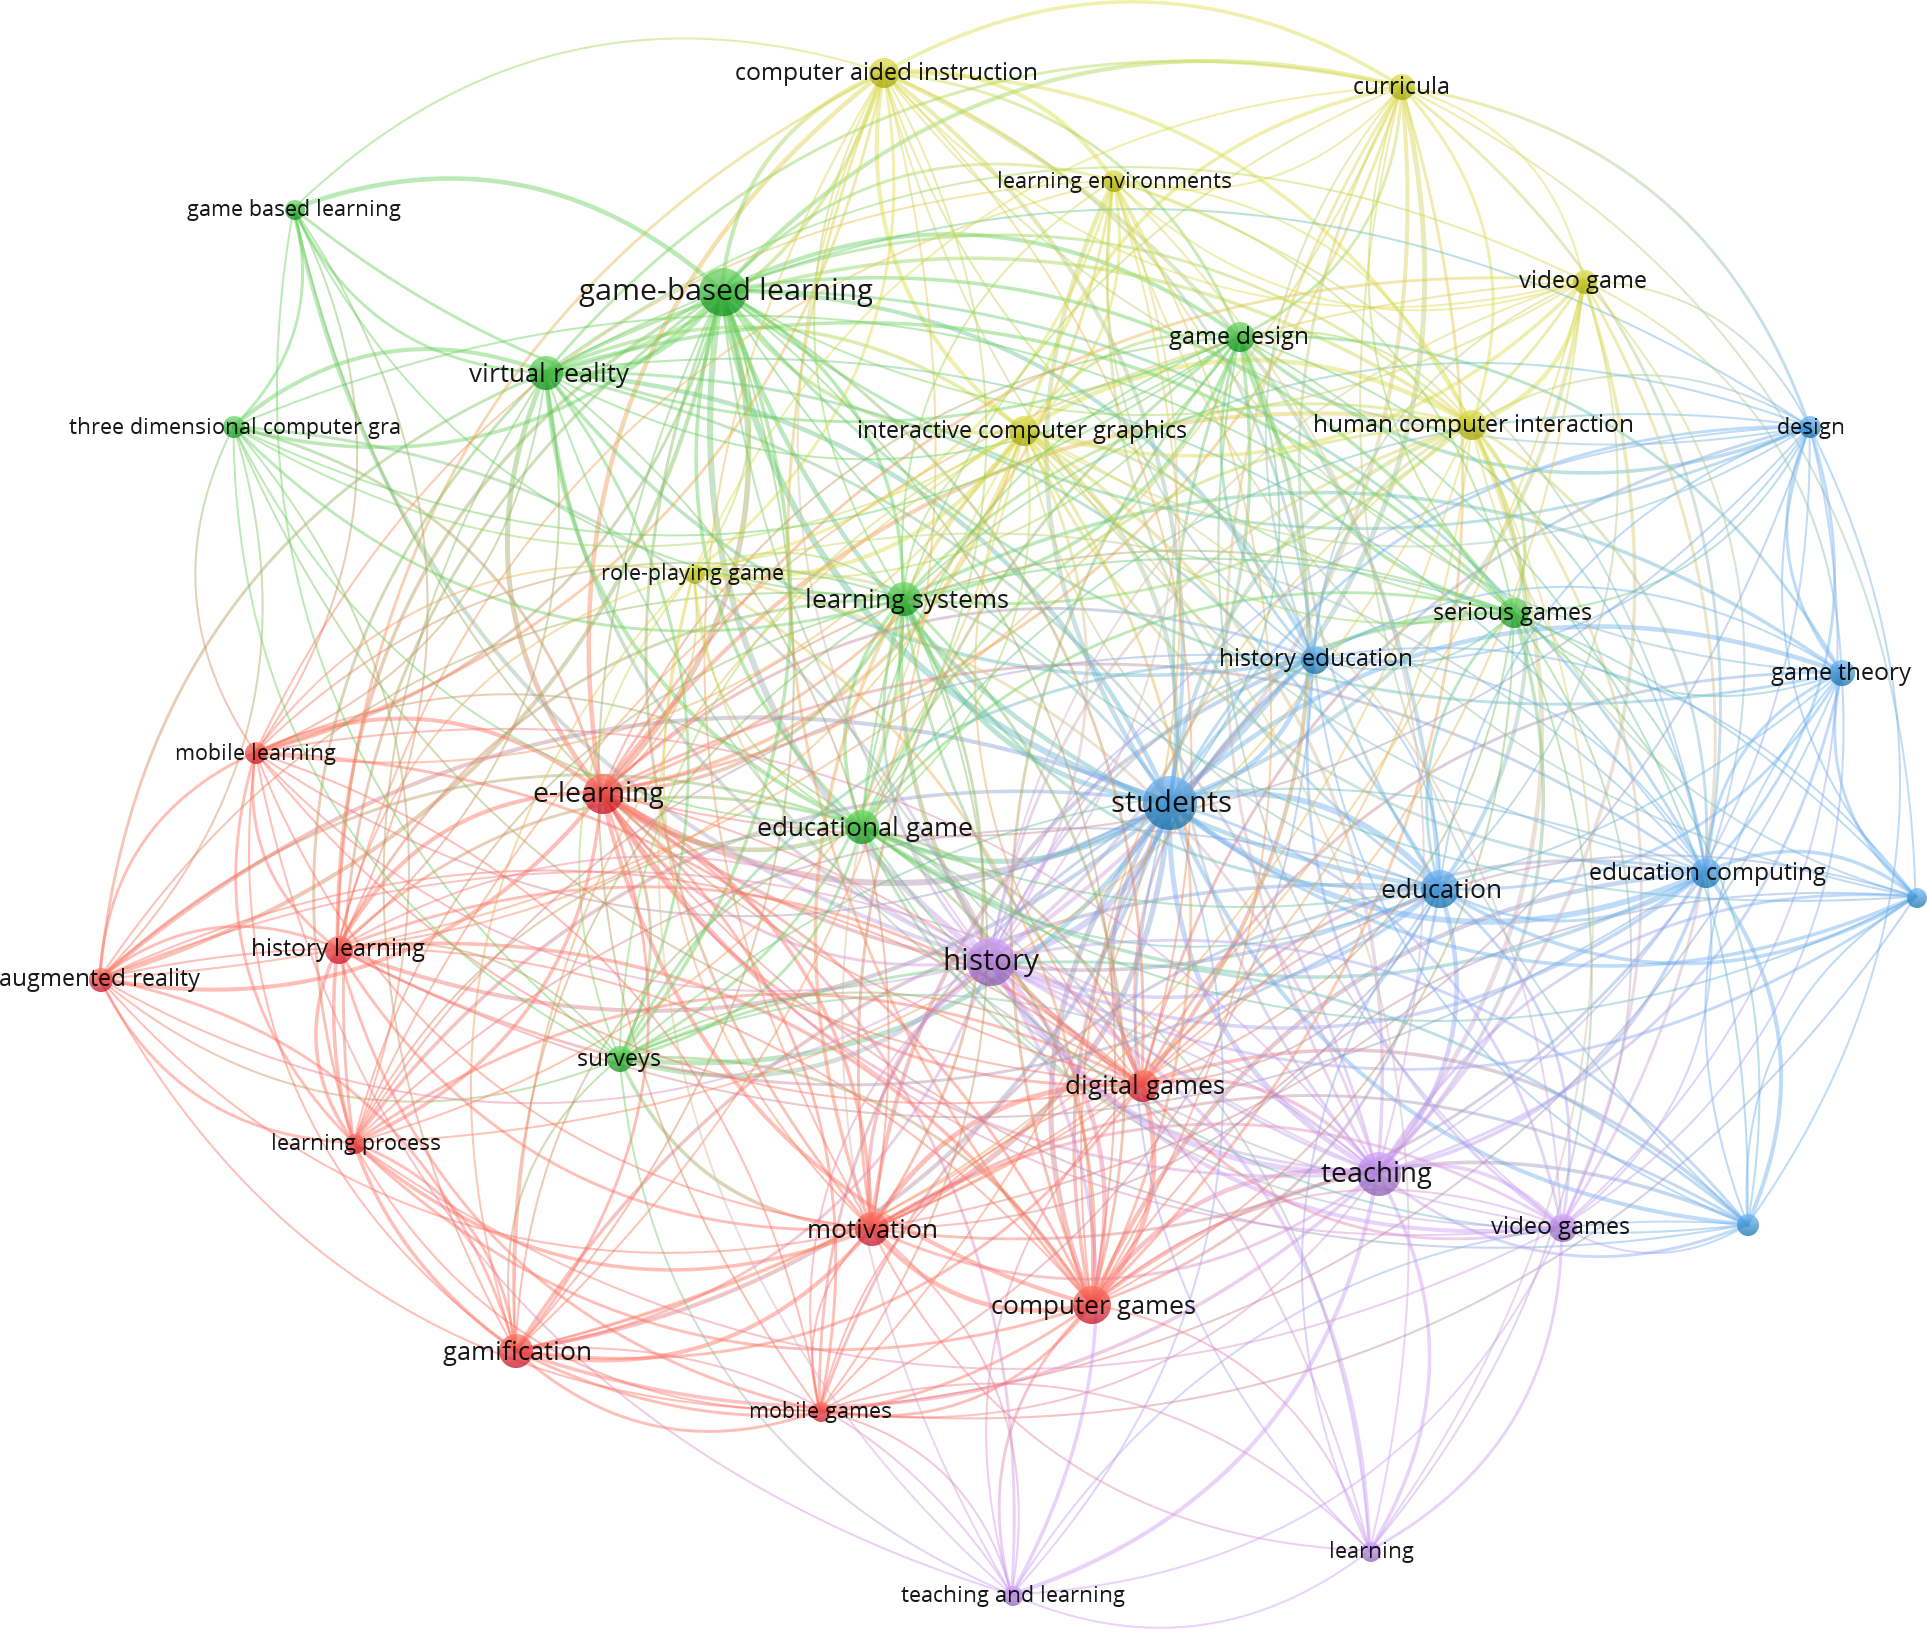
\includegraphics[width=1\linewidth]{aims_result.png}
% \caption{Aims bibliographic network.}
%% \caption{A holistic view of all clusters.}
% \label{fig:aims_result}
%\end{figure}
%
%
%\begin{figure}
% \centering
% 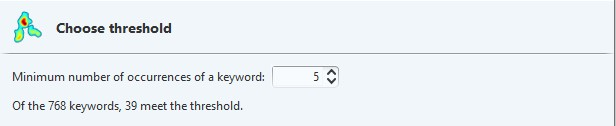
\includegraphics[width=1\linewidth]{aims_cmap_1.jpg}
% 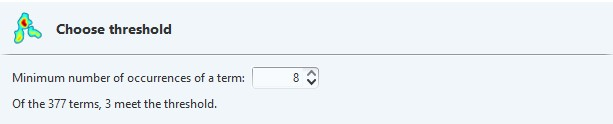
\includegraphics[width=1\linewidth]{aims_cmap_2.jpg}
% \caption{Tuning of threshold and the number of terms.}
% \label{fig:aims_create_map}
%\end{figure}
%
%\begin{figure}
% \centering
% 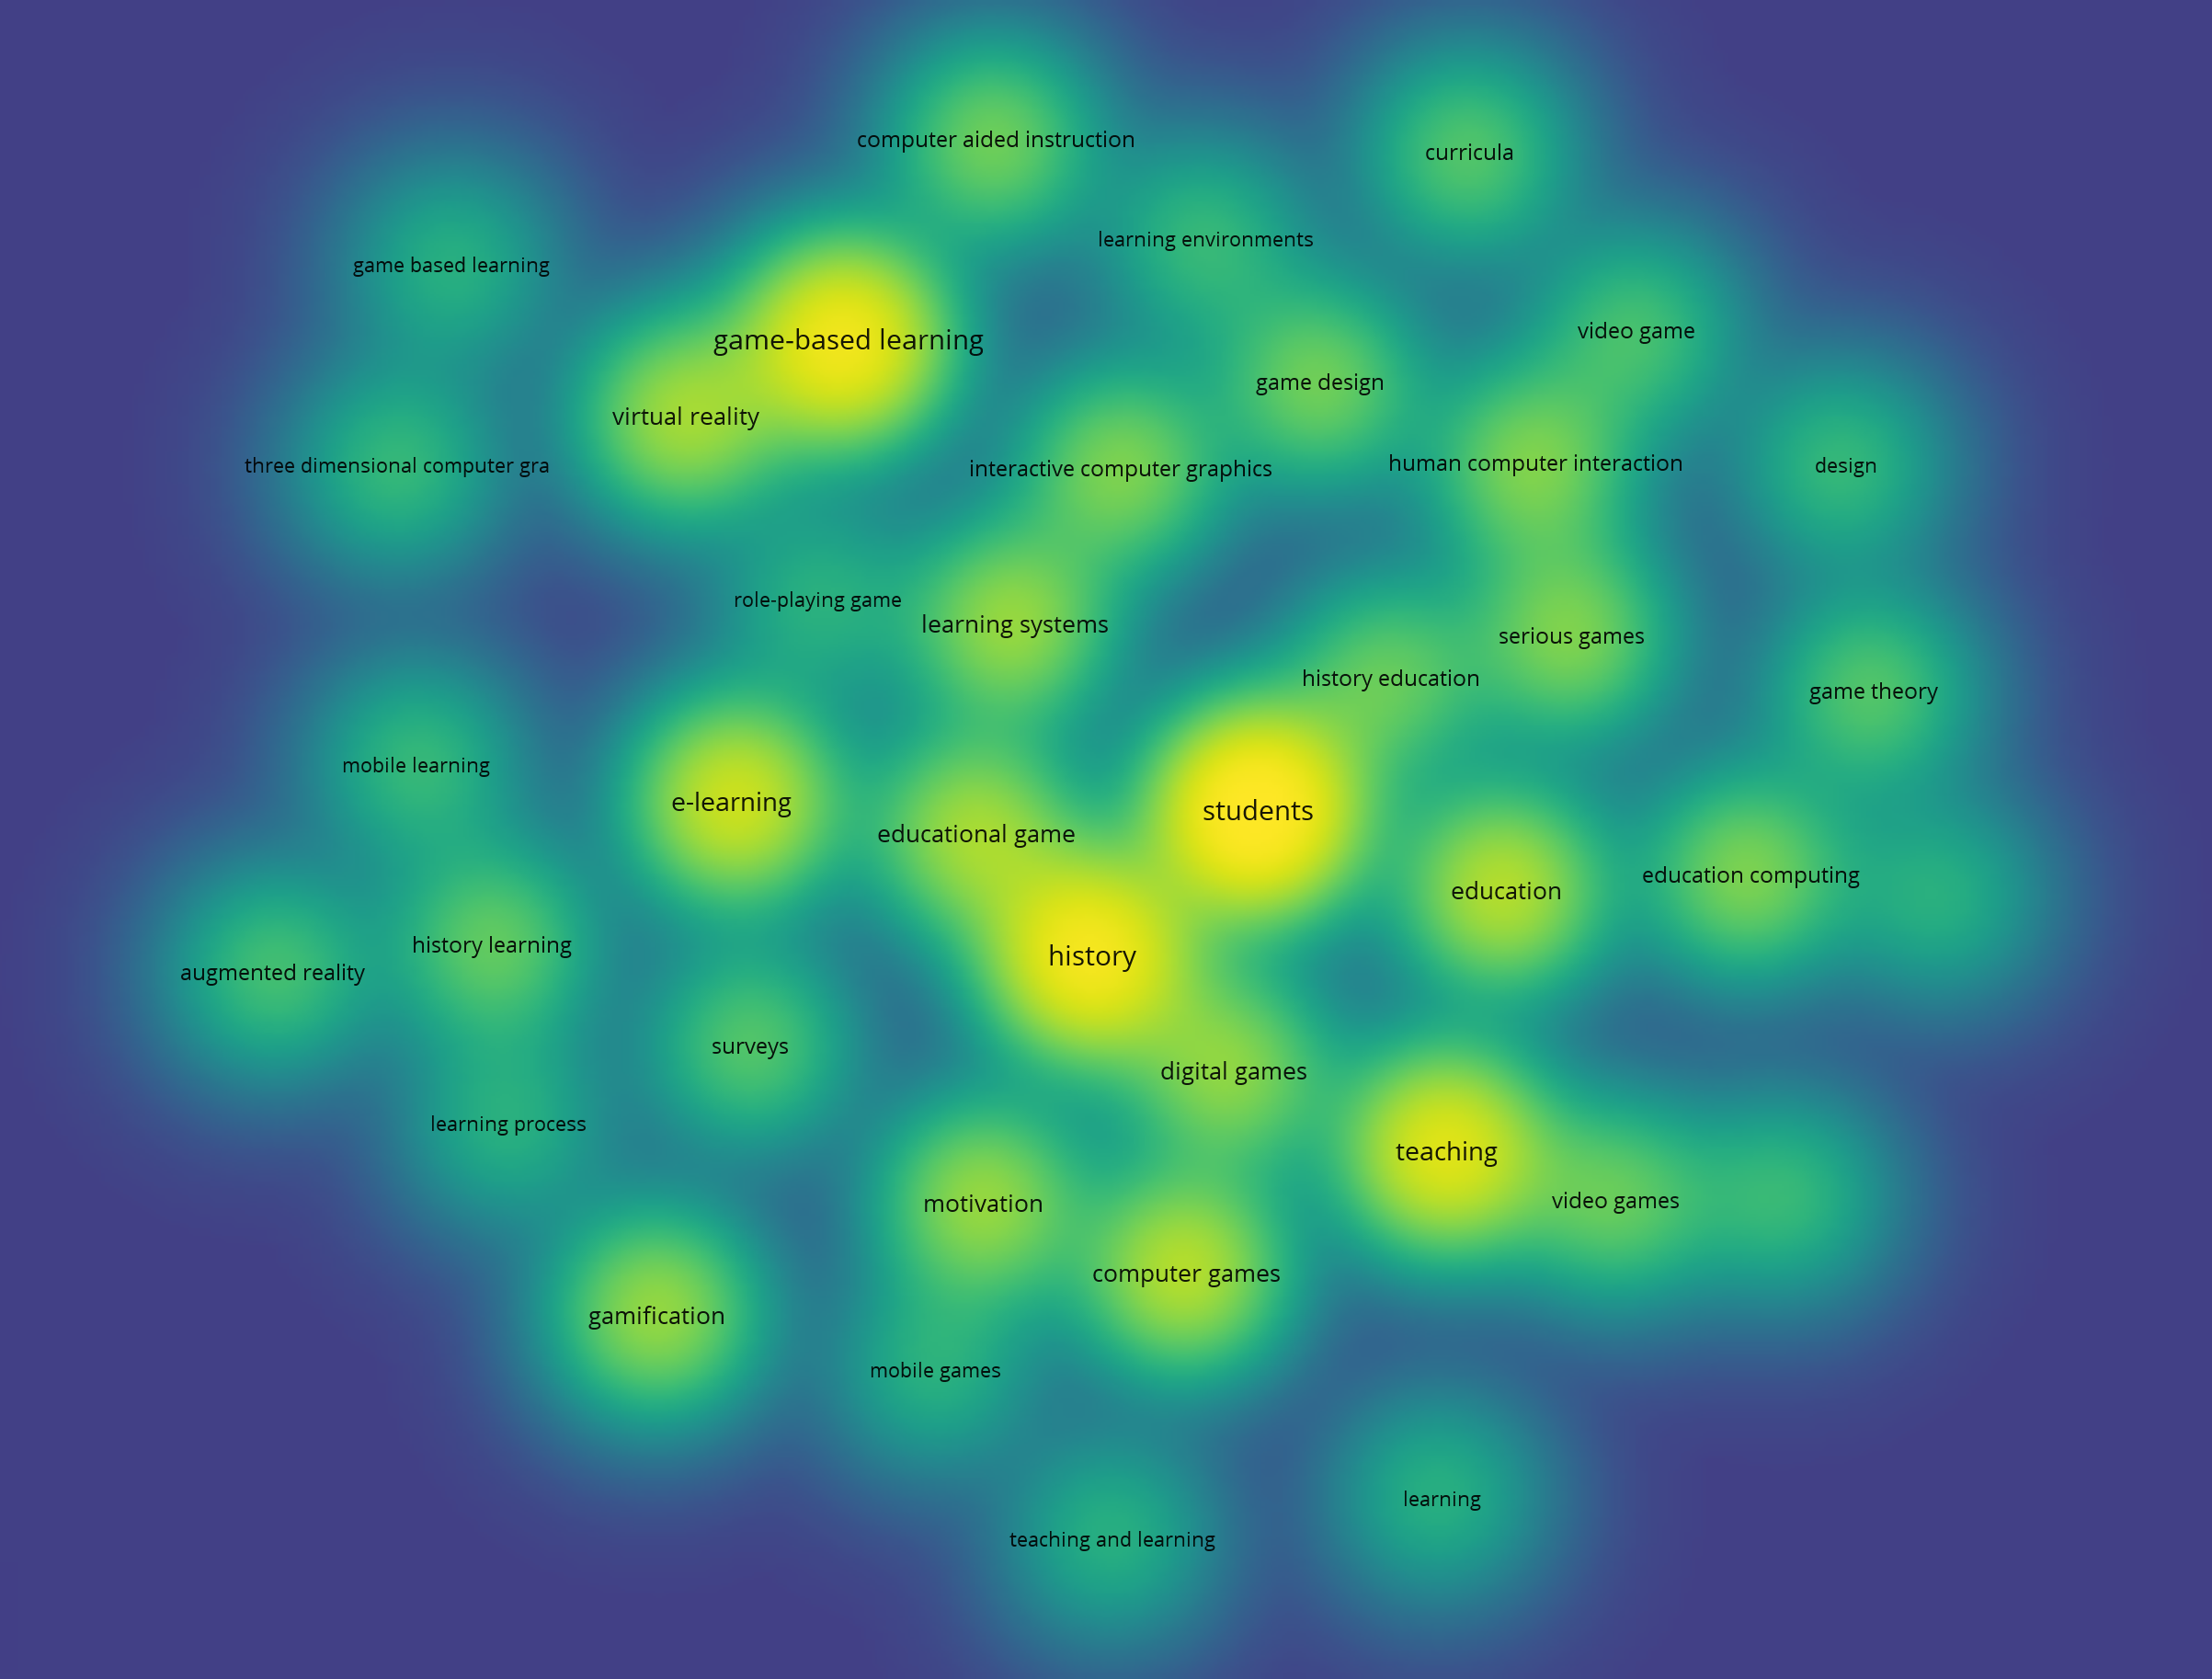
\includegraphics[width=1\linewidth]{aims_density.png}
% \caption{Density visualisation of aims bibliographic network.}
% \label{fig:aims_density}
%\end{figure}
%
%\begin{enumerate}[noitemsep]
% \item {First cluster (in red, major) is shown in Figure~\ref{fig:aims_red_cluster}}. Red cluster is focused on \textit{augmented reality} and \textit{history learning}, along with related concepts like \textit{gamification}, \textit{mobile games}, \textit{computer games}, and other vital parts of the gamification methodology. Terms like \textit{learning process} and \textit{history learning} imply studies examining the pros and cons of gamification methods in an educational context.
% One term of the green cluster was closely related to the red cluster: \textit{surveys}, what probably, represent educational methodology part. 
% 
% \item {Second cluster (in green) is shown in Figure~\ref{fig:aims_green_cluster}}. The red group focuses on the concept of \textit{game-based learning} and the technical aspects of its implementation. Key related terms include \textit{learning systems} \textit{educational game}, \textit{three dimensional computer graphic}, \textit{game design}, \textit{serious game}, and \textit{virtual reality}.
% One term of the yellow cluster was closely related to the green cluster: \textit{role-playing game}, what probably, represent game part 
% 
% \item {Third cluster (in blue, minor) is shown in Figure~\ref{fig:aims_blue_cluster}}. The blue group is focused on the \textit{student}, \textit{education}, and \textit{game theory}, indicating the education computing connects history teaching, digital games and educational games in learning courses.
%
% \item {Fourth cluster (in purple) is shown in Figure~\ref{fig:aims_purpule_cluster}}. The purple group is incorporate \textit{learning}, \textit{teaching}, and \textit{video games}, connecting all clusters around \textit{history}.
%
% \item {Fifth cluster (in yellow) is shown in Figure~\ref{fig:aims_yellow_cluster}}. Yellow cluster is focused on \textit{interactive computer graphics} and \textit{human computer interaction}, along with related concepts like \textit{learning environments}, \textit{video game}, \textit{computer aided instruction}, and other vital parts of the gamification methodology. Terms like \textit{learning process} and \textit{history learning} imply studies examining the pros and cons of gamification methods in an educational context.
% One term of the green cluster was closely related to the yellow cluster: \textit{game design}, what probably, connecting with computer interaction part. 
% 
%\end{enumerate} 
%
%\begin{figure}[ht!]
% \centering
% 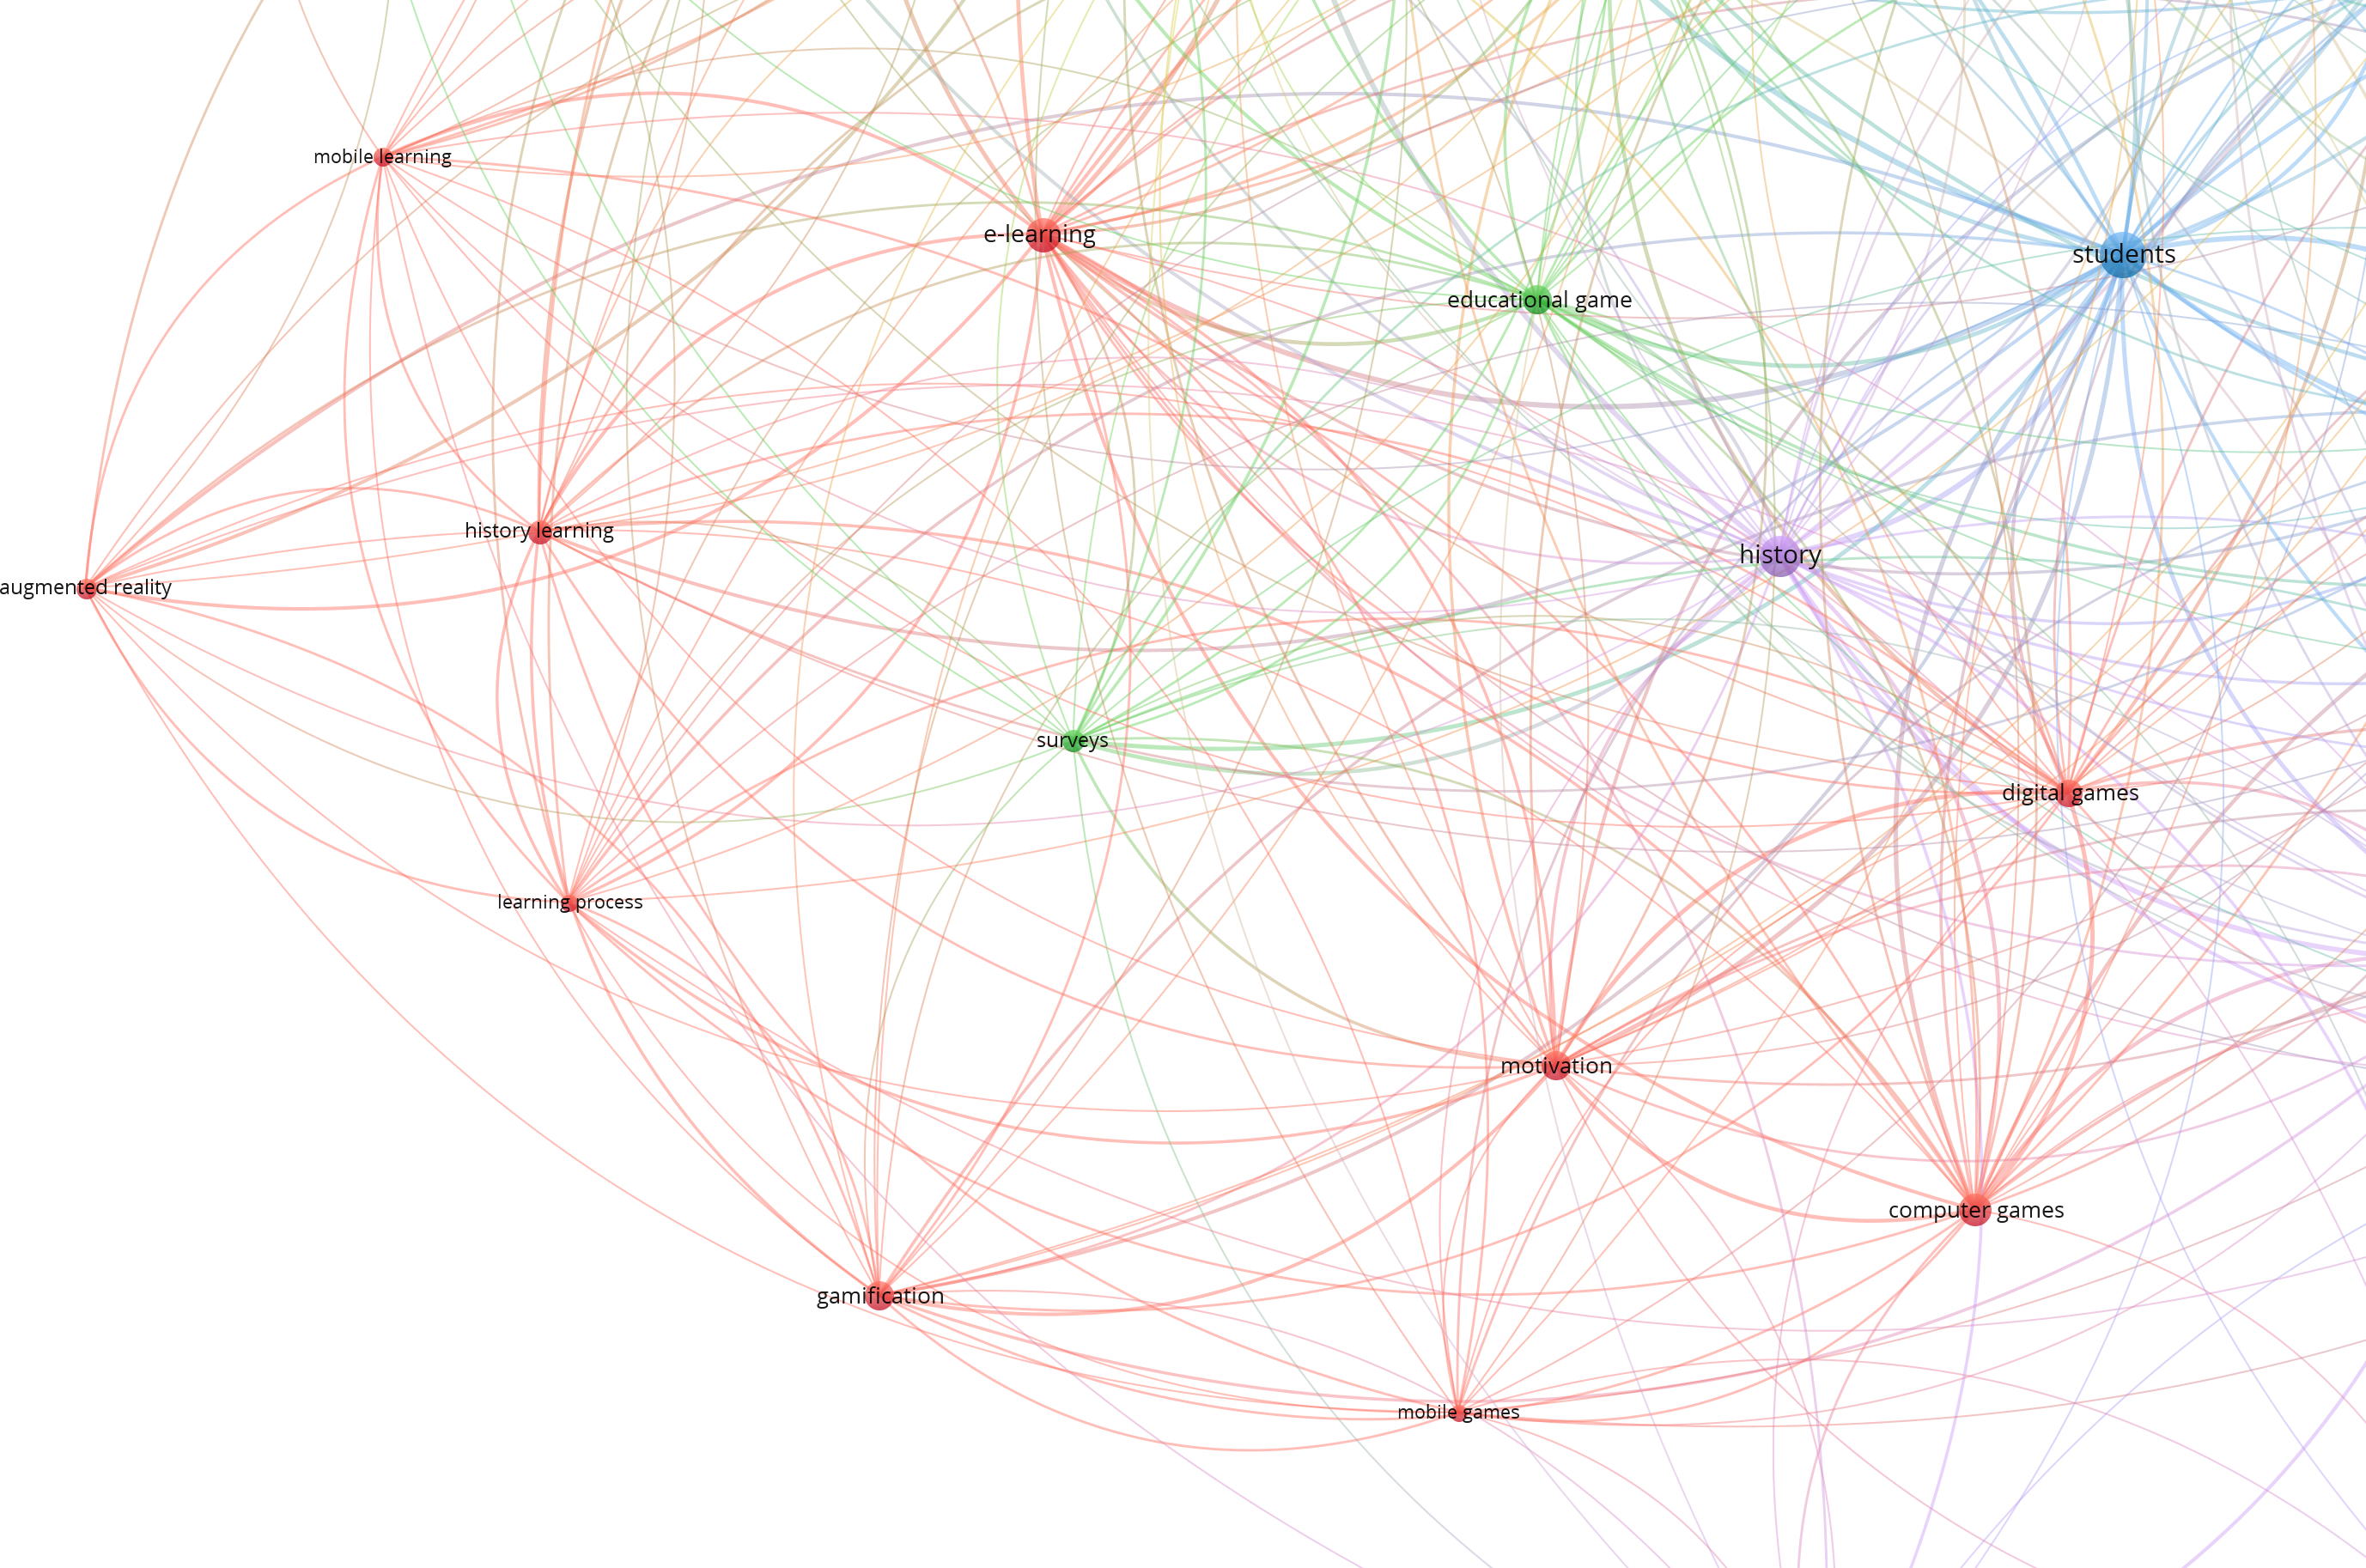
\includegraphics[width=\linewidth]{aims_red_cluster.png}
% \caption{Cluster of augmented reality and history learning.}
% \label{fig:aims_red_cluster}
%\end{figure}
%
%\begin{figure}[ht!]
% \centering
% 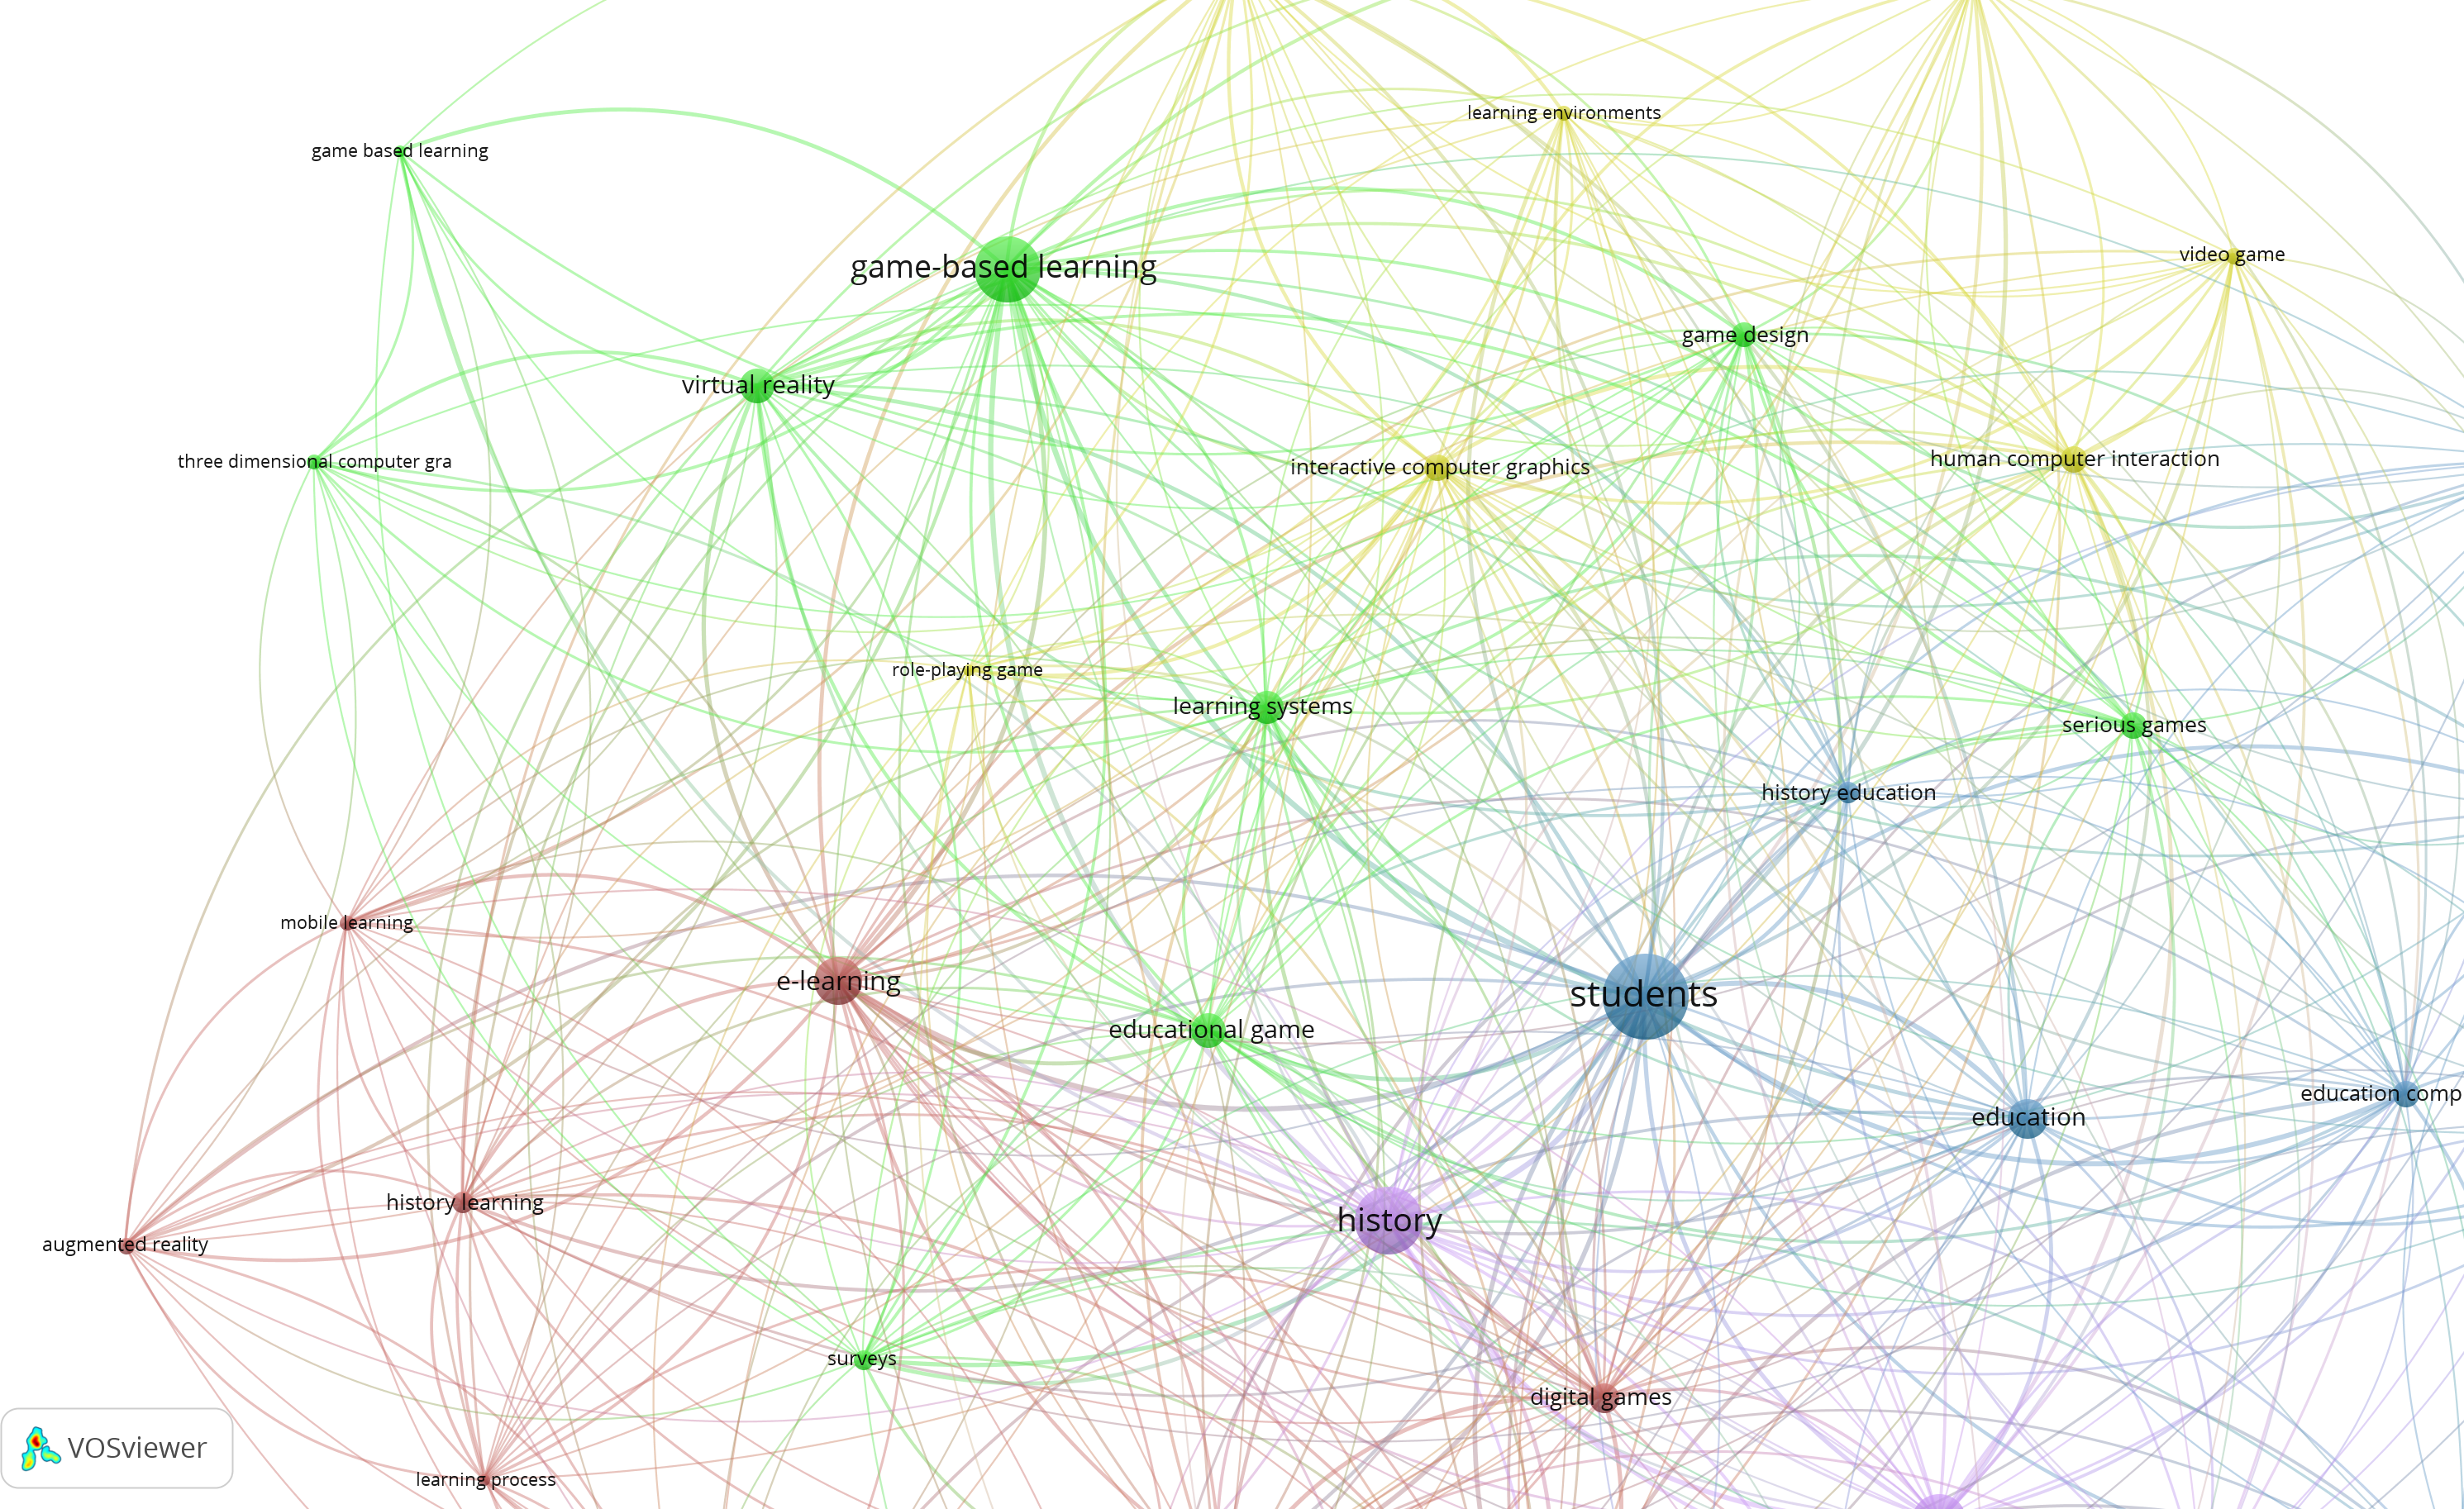
\includegraphics[width=\linewidth]{aims_green_cluster.png}
% \caption{Cluster of game-based learning and the technical aspects of its implementation}
% \label{fig:aims_green_cluster}
%\end{figure}
%
%\begin{figure}[ht!]
% \centering
% 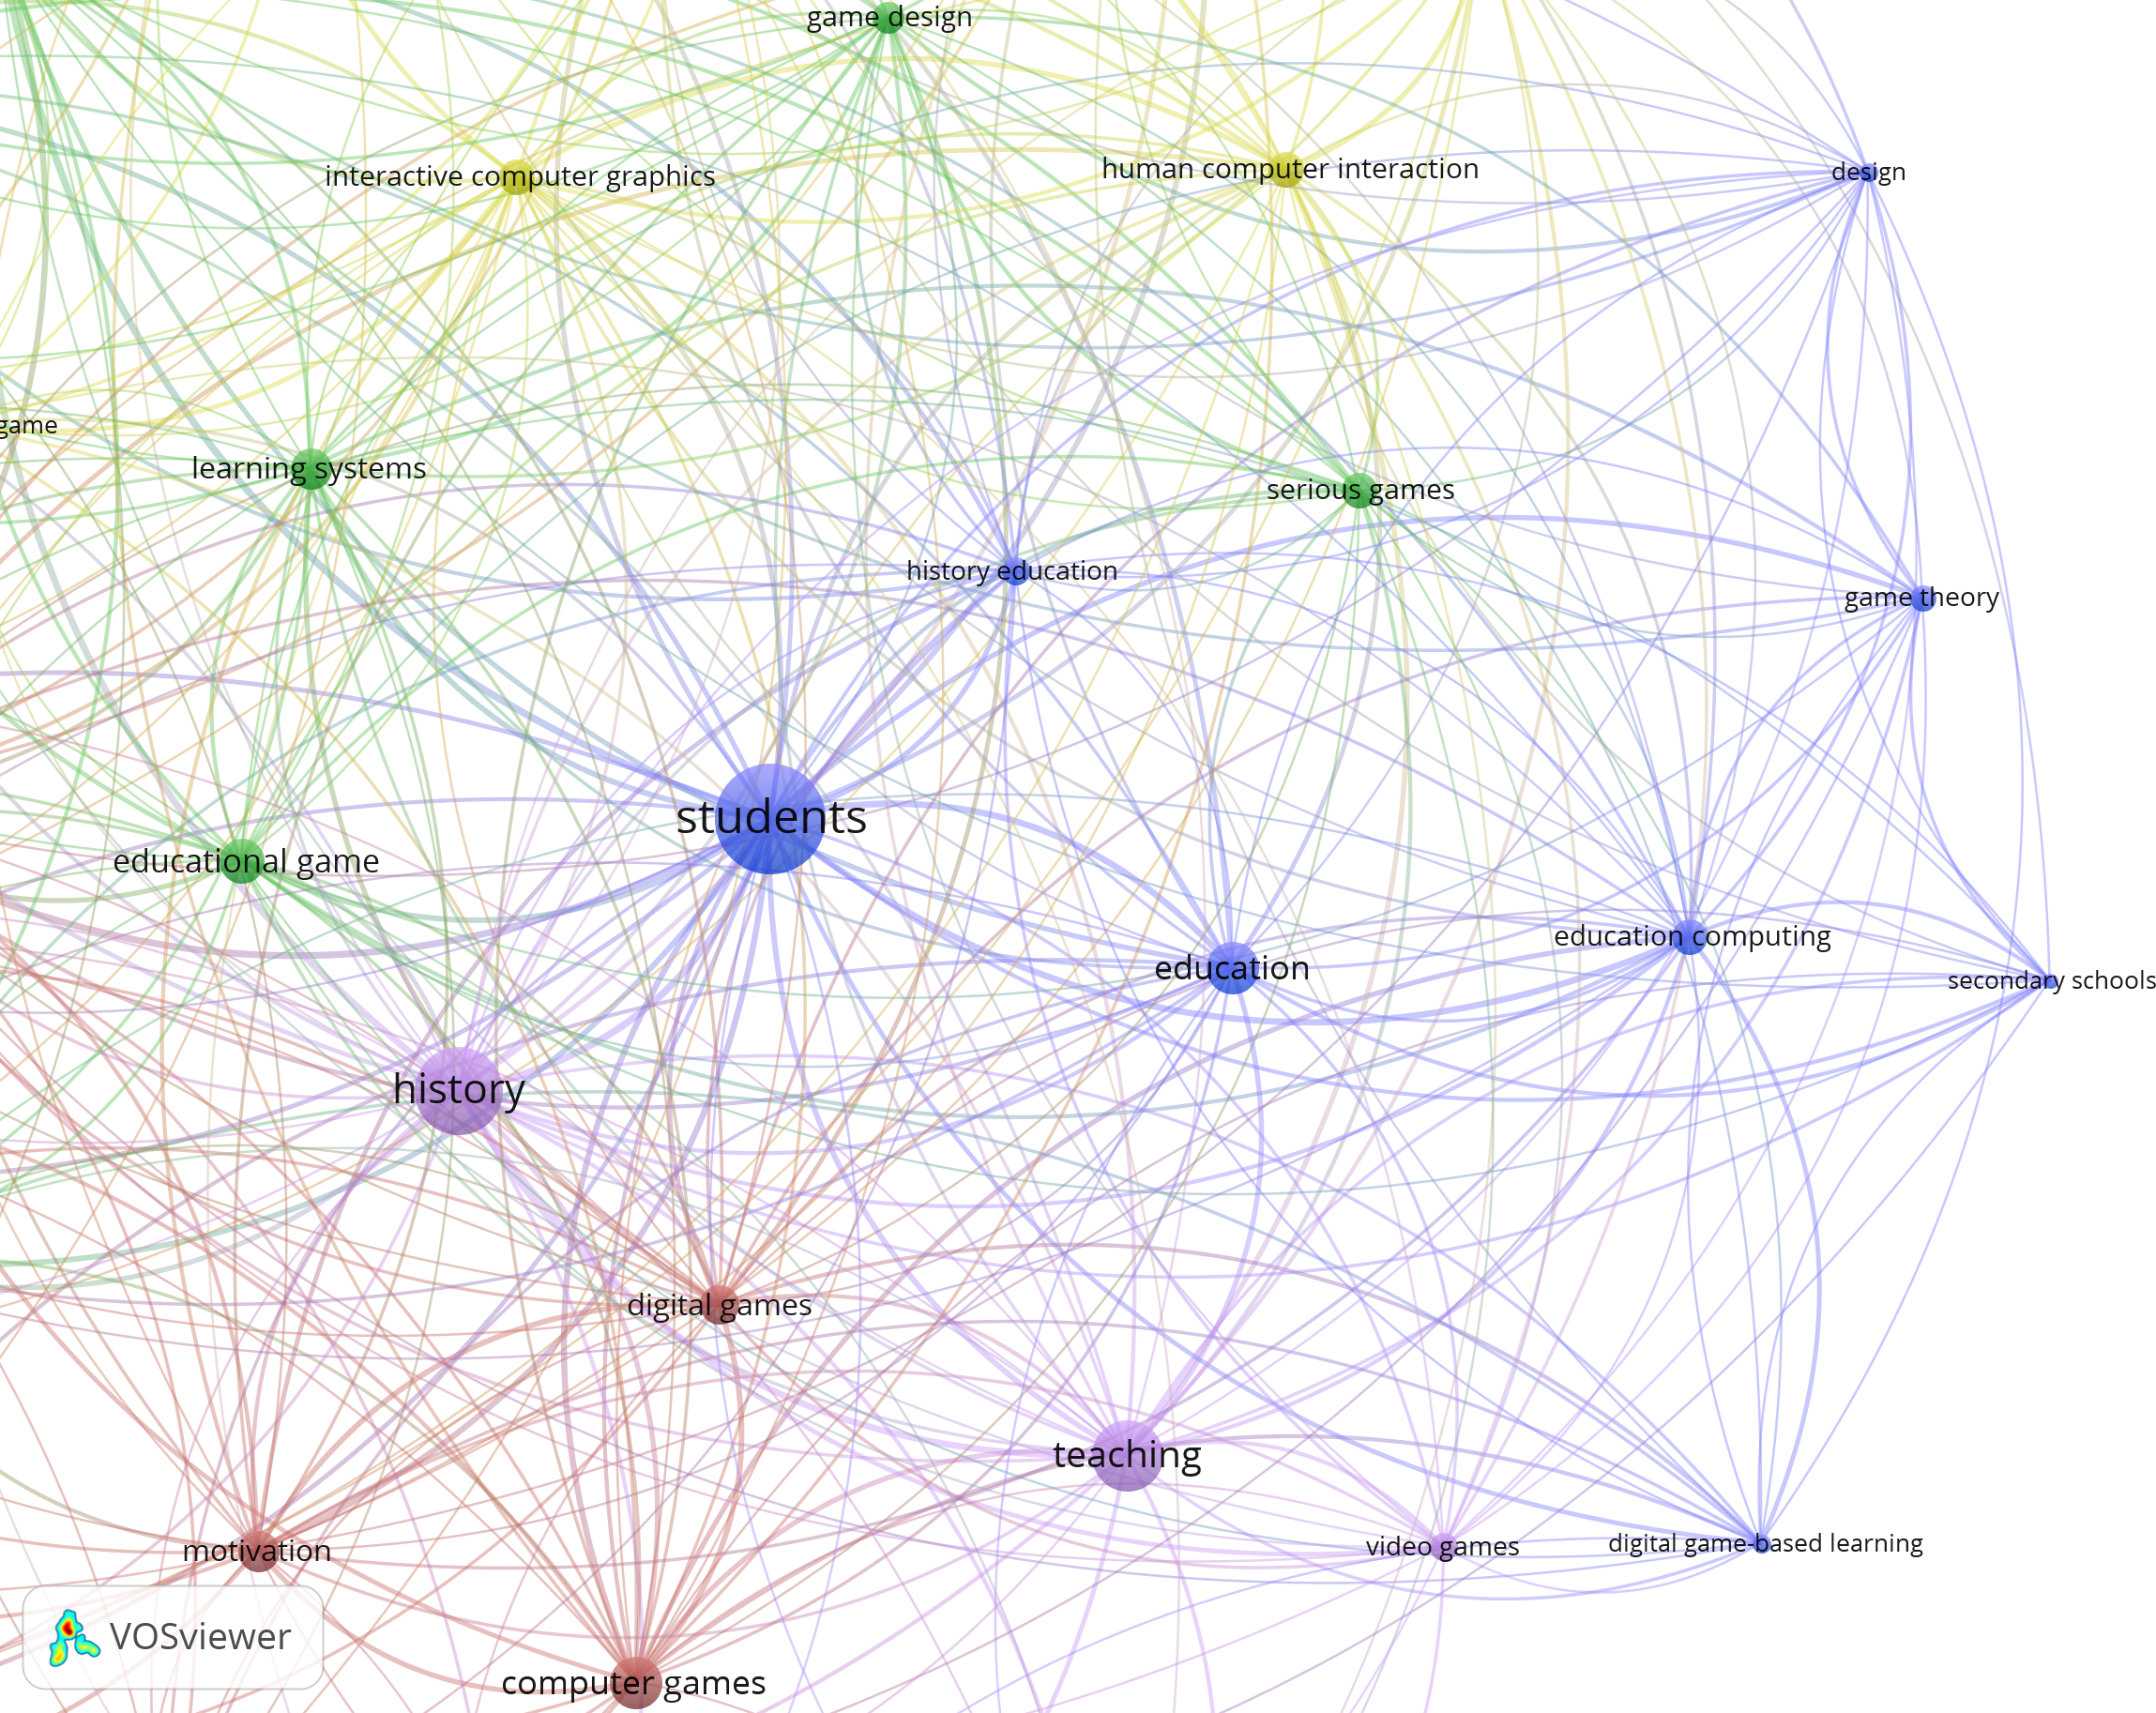
\includegraphics[width=\linewidth]{aims_blue_cluster.png}
% \caption{Cluster of course learning outcomes in aims bibliographic network.}
% \label{fig:aims_blue_cluster}
%\end{figure}
%
%\begin{figure}[ht!]
% \centering
% 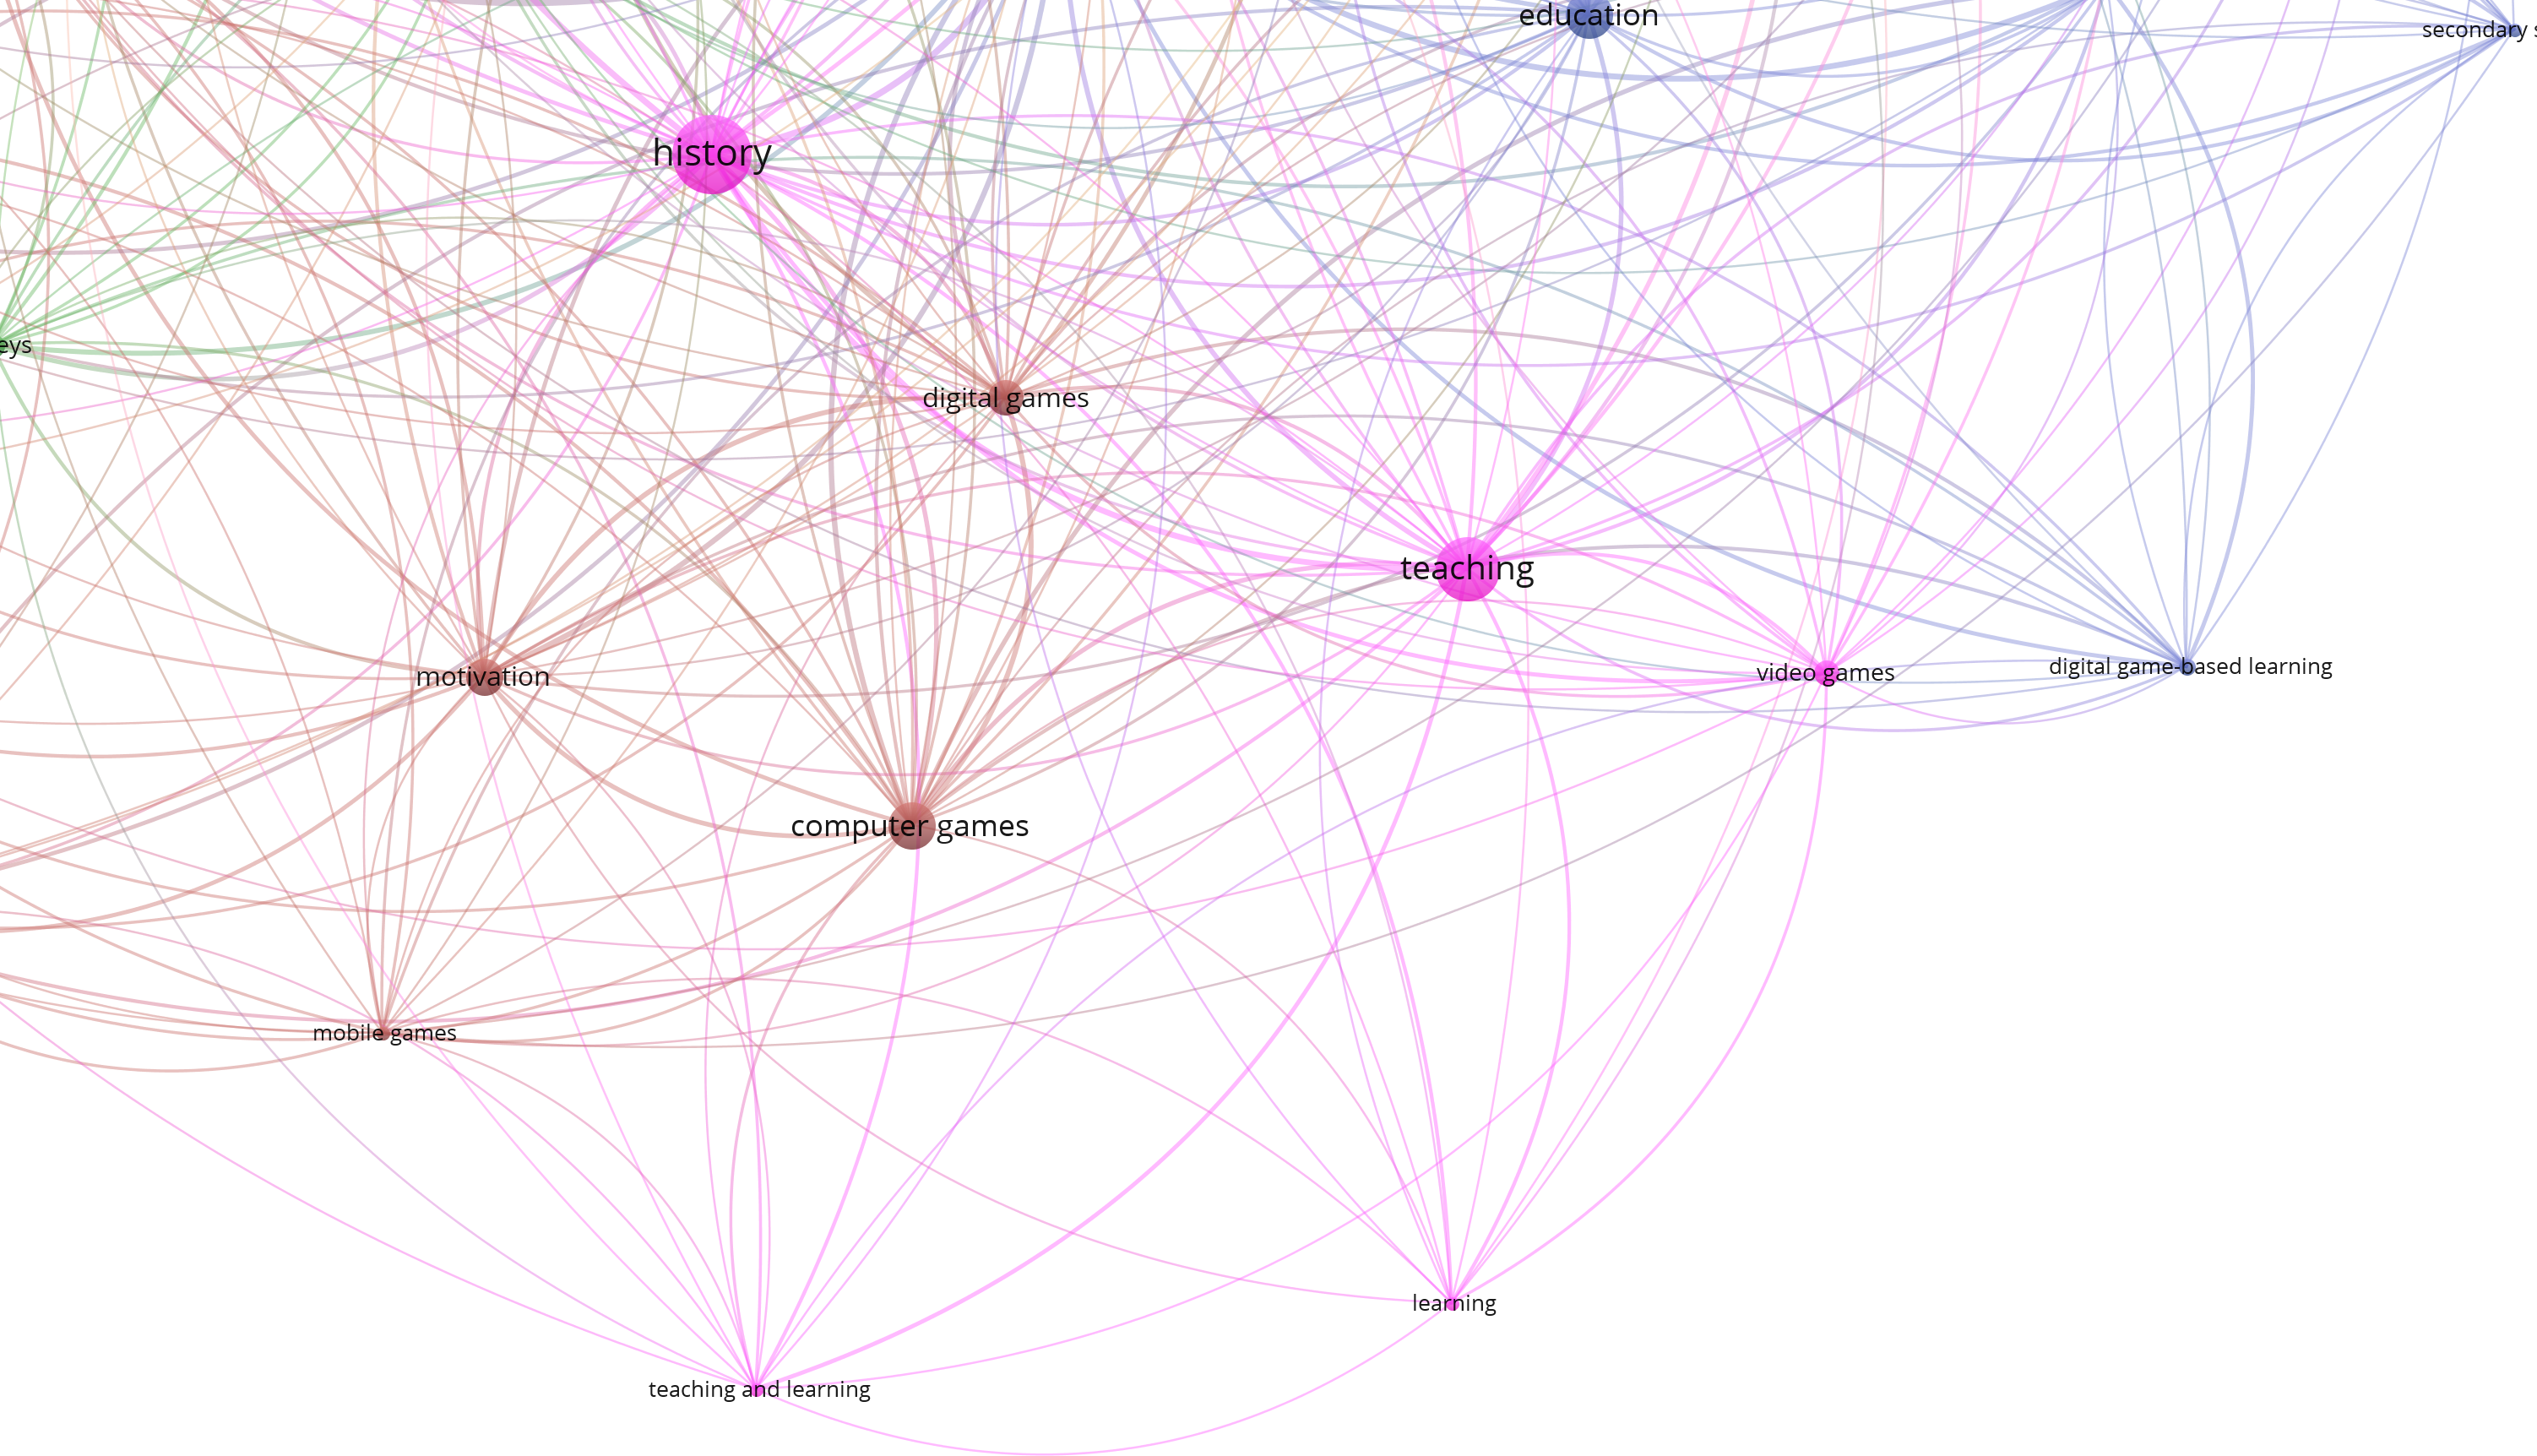
\includegraphics[width=\linewidth]{aims_purpule_cluster.png}
% \caption{Cluster of course learning outcomes in aims bibliographic network.}
% \label{fig:aims_purpule_cluster}
%\end{figure}
%
%\begin{figure}[ht!]
% \centering
% 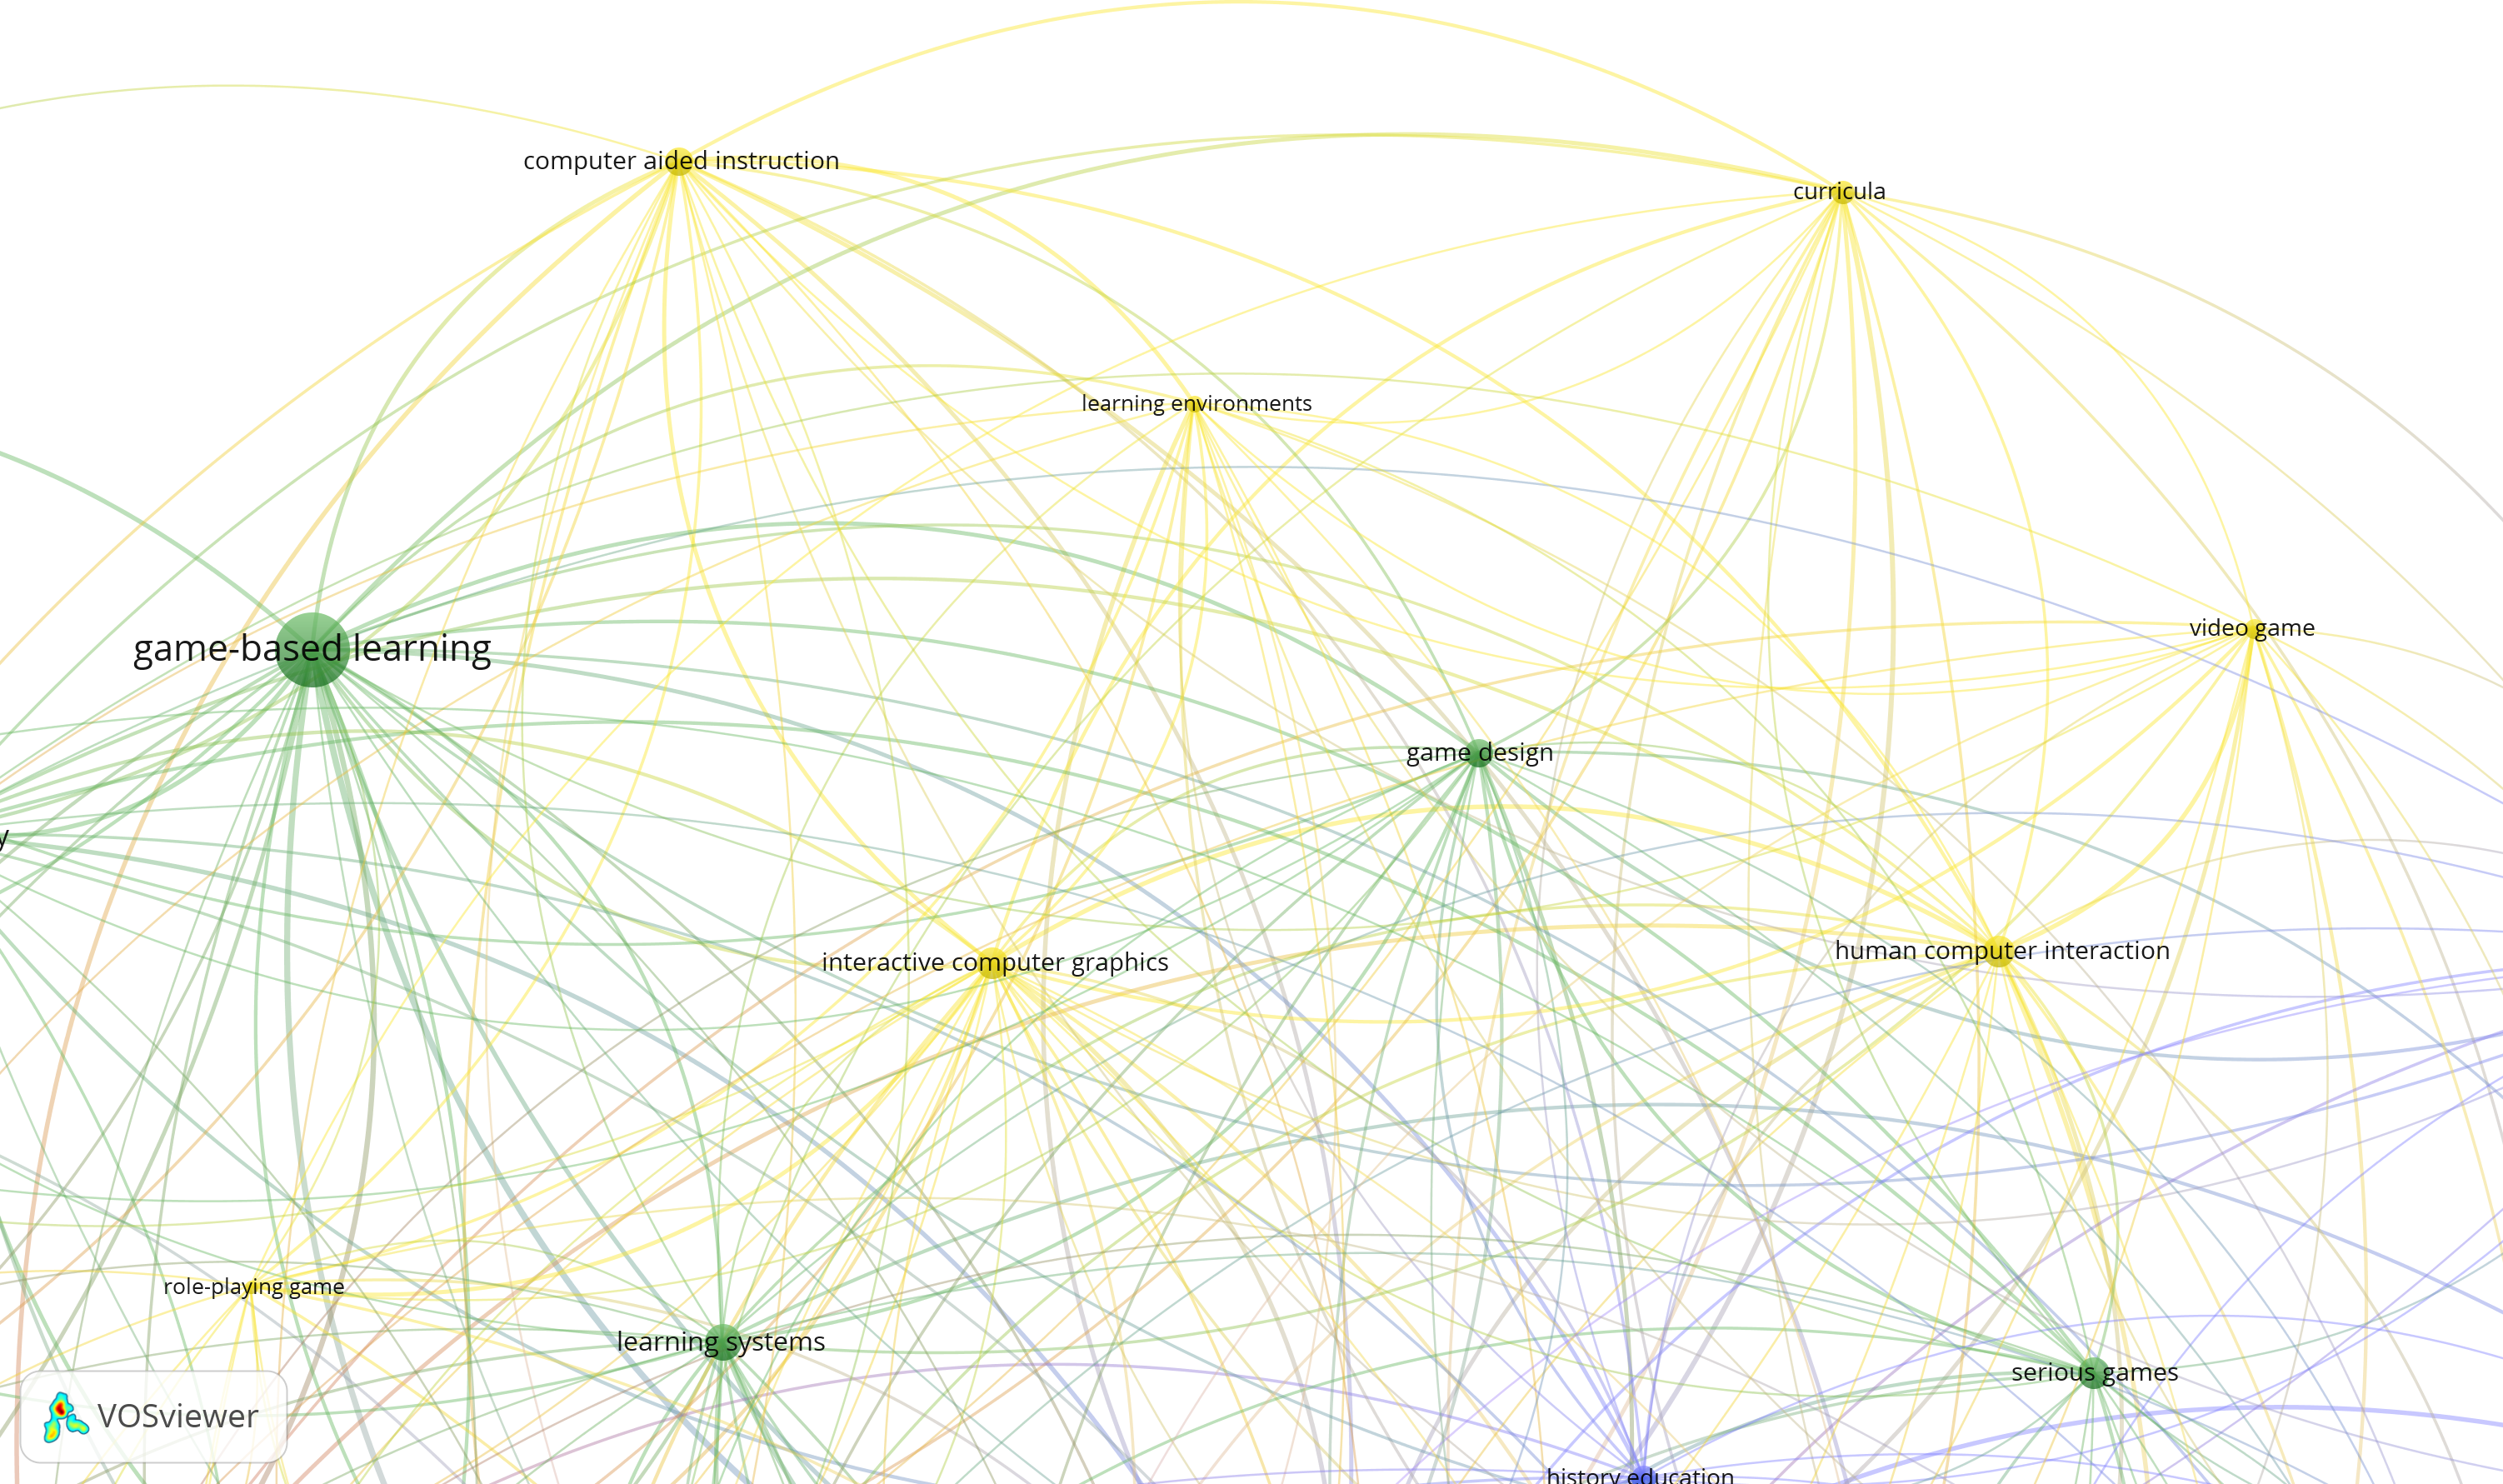
\includegraphics[width=\linewidth]{aims_yellow_cluster.png}
% \caption{Cluster of course learning outcomes in aims bibliographic network.}
% \label{fig:aims_yellow_cluster}
%\end{figure}
%
%While only the analysis of clustering would show us how they are grouped, the year distribution is more precise. The analysis showed a clear temporal trend from studying specific gamification methods to the learning process more generally and then to serious game (Table~\ref{aims_table}): 
%
%\begin{enumerate}[noitemsep]
% \item The \textbf{early exploration stage} (2004--2012) is characterized by initial investigations into using computer games for history education. Keywords such as \textit{computer game}, \textit{educational game}, and \textit{learning} dominate this period. Research focused on foundational questions about whether games could effectively support history learning.
%
% \item The \textbf{narrative and engagement stage} (2013--2017) shows a shift towards examining how game narratives and storytelling can enhance historical understanding. Keywords like \textit{history learning}, \textit{video game}, \textit{motivation}, and \textit{serious game} reflect growing interest in leveraging narrative elements for historical empathy and engagement.
%
% \item The \textbf{immersive technology stage} (2018--2024) represents the adoption of emerging technologies. Keywords such as \textit{augmented reality}, \textit{virtual reality}, \textit{gamification}, and \textit{mobile game} indicate a broadening of technological approaches and a more systematic integration of game design principles into history education.
%\end{enumerate}
%
%
%The two bibliometric maps (based on paper aims and titles) have some key similarities and differences:
%
%\begin{itemize}[noitemsep]
% \item
%The major cluster (red) in both maps emphasizes the learning process, especially gamification and game-based learning approaches.
% \item
%The second cluster (green) in both maps highlights educational game design and the technical aspects of implementation.
% \item
%The aims map emphasizes specific gamification practices (augmented reality, motivation) more strongly, while the titles map focuses more on participant outcomes and educational contexts.
% \item
%A notable difference is the inclusion of \textit{empirical study} and \textit{case study} in the titles map. However, their impact (occurrence and link strength) is relatively minor compared to dominant terms such as \textit{game-based learning} and \textit{history}, which play central roles in both maps.
% \item
%The minor (blue) cluster differs~-- in the aims map, it centres on student engagement and history learning, while in the titles map, it focuses more narrowly on effects on student performance and educational outcomes.
%\end{itemize}
%
%\begin{table}[ht]
%\caption{Distribution of keywords by clusters (from aims bibliometric network).}
%\label{maptable}
%\setlength \tabcolsep {0.25\tabcolsep }
%
%\begin{tabular}{|l|c|c|c|}
%\hline
%\hfill \textbf{Keyword} & \textbf{Total link strength} & \textbf{Occurrences} & \textbf{Average publication year}\\ \hline
%\cellcolor{red!35}{gamification} & 185 & 62 & 2017.8 \\
%\cellcolor{red!35}{history learning} & 142 & 48 & 2016.5 \\
%\cellcolor{red!35}{augmented reality} & 78 & 22 & 2018.2 \\
%\cellcolor{red!35}{mobile game} & 65 & 18 & 2017.1 \\
%\cellcolor{red!35}{computer game} & 58 & 16 & 2012.4 \\
%\cellcolor{red!35}{motivation} & 52 & 15 & 2016.9 \\
%\cellcolor{red!35}{engagement} & 48 & 14 & 2018.6 \\ \hline
%\cellcolor{green!35}{game-based learning} & 198 & 68 & 2015.3 \\
%\cellcolor{green!35}{educational game} & 125 & 40 & 2016.1 \\
%\cellcolor{green!35}{serious game} & 112 & 35 & 2015.8 \\
%\cellcolor{green!35}{virtual reality} & 72 & 20 & 2018.4 \\
%\cellcolor{green!35}{game design} & 65 & 19 & 2016.7 \\
%\cellcolor{green!35}{three-dimensional computer graphics} & 45 & 12 & 2014.9 \\ \hline
%\cellcolor{blue!30}{student} & 168 & 55 & 2016.2 \\
%\cellcolor{blue!30}{education} & 135 & 45 & 2015.6 \\
%\cellcolor{blue!30}{learning} & 98 & 32 & 2015.4 \\
%\cellcolor{blue!30}{teaching} & 82 & 28 & 2014.8 \\ \hline
%\cellcolor{purple!30}{video game} & 75 & 21 & 2016.3 \\
%\cellcolor{purple!30}{history} & 205 & 72 & 2015.9 \\ \hline
%\cellcolor{yellow!50}{interactive computer graphics} & 42 & 11 & 2013.5 \\
%\cellcolor{yellow!50}{human computer interaction} & 38 & 10 & 2015.2 \\
%\cellcolor{yellow!50}{learning environment} & 35 & 9 & 2017.4 \\ \hline
%\end{tabular}
%\label{aims_table}
%\end{table}
%
%%PRISMA 2020 step 18
%\subsection{Overview of risk of bias assessment}
%
%This section presents the assessment of risk of bias for the 74 studies included in this systematic review, based on an adapted ROBIS framework across three domains: participant selection (Domain~1), data collection and analysis (Domain~2), and interpretation and reporting (Domain~3).
%
%Figure~\ref{fig:rob_summary} summarises the risk of bias judgements across all three domains and overall. The majority of studies (62 out of 74, 83.8\%) were rated as having high overall risk of bias, primarily due to inadequate sample sizes, absent control groups, unvalidated measurement instruments, and missing limitations discussions. Only one study was judged to have low overall risk of bias.
%
%\begin{figure}[ht!]
%\centering
%\begin{tikzpicture}
%\begin{axis}[
% width=14cm,
% height=6cm,
% xbar stacked,
% bar width=12pt,
% xlabel={Number of studies},
% symbolic y coords={Overall,Domain 3,Domain 2,Domain 1},
% ytick=data,
% legend style={at={(0.5,-0.2)}, anchor=north, legend columns=4},
% xmin=0, xmax=80,
% enlarge y limits=0.25,
% nodes near coords align={horizontal},
%]
%\addplot[fill=red!70] coordinates {(62,Overall) (42,Domain 3) (47,Domain 2) (63,Domain 1)};
%\addplot[fill=yellow!70] coordinates {(9,Overall) (14,Domain 3) (10,Domain 2) (6,Domain 1)};
%\addplot[fill=gray!50] coordinates {(2,Overall) (5,Domain 3) (8,Domain 2) (5,Domain 1)};
%\addplot[fill=green!60] coordinates {(1,Overall) (13,Domain 3) (9,Domain 2) (0,Domain 1)};
%\legend{High, Moderate, Unclear, Low}
%\end{axis}
%\end{tikzpicture}
%\caption{Summary of risk of bias assessment across the three domains and overall ($n=74$). Domain~1: participant selection; Domain~2: data collection and analysis; Domain~3: interpretation and reporting.}
%\label{fig:rob_summary}
%\end{figure}
%
%\subsubsection{Methodological quality assessment}
%
%%\subsection{Sample Size Limitations}
%
%A substantial proportion of included studies exhibited significant risk of bias due to inadequate sample sizes. Of the 62 studies reporting participant numbers, 41 (66.1\%) utilized sample sizes below 50 participants, raising concerns about statistical power and reliability of findings.
%
%Studies with particularly small samples included: \citet{1Barbatsis201159} ($n=17$), \citet{6Czerwinski2018} ($n=30$ postgraduate students in a single discipline), \citet{13Humpire2022} (sample size not specified), \citet{21Ghulamani2017} ($n=8$ teachers with classroom observations), \citet{22Nugroho2020149} ($n=5$ respondents), \citet{25Repantis2011502} (8 student designers; sample size not formally reported), \citet{50Lye2013} ($n=5$ first-year students), and \citet{51Ardito2007} ($n=4$ for preliminary evaluation). These small sample sizes substantially limit the generalizability of findings and increase the likelihood of Type~II errors.
%
%Several studies acknowledged sample size as a limitation. \citet{5kazanidis2018alpha} explicitly noted ``limited sample size'' as a constraint, while \citet{11Ternblad2023115} identified insufficient sample size for robust quantitative analysis. \citet{42Huffer201581} similarly recognized that their 11 student teams represented a limited sample for drawing broad conclusions. \citet{63Liu2021} reported only 12 participants, with authors acknowledging this as insufficient for meaningful statistical analysis.
%
%\subsubsection{Research design concerns}
%
%Significant heterogeneity in research designs contributed to varying levels of bias risk across studies. Approximately 25 studies (31\%) lacked comparison groups entirely, relying solely on pre-post single-group designs without controls. This design limitation was particularly evident in \citep{9Lin2018, 16Chen201447, 19Chou2019, 22Nugroho2020149, 45Yu2016727, 52Lin2011265, 63Liu2021, 64Hsu201324, 67Lin201296, 77Ramansyah2021}, where the absence of control conditions precludes causal inference regarding the effects of the intervention.
%
%\citet{3Watson2011466, 12Gilbert2019108, 14Forsyth2023, 46Stirling2022, 60Hoy2018, 65Razak201139, 71lynch2015pedagogical} employed purely qualitative methodologies without quantitative outcome measures. While qualitative approaches provide valuable insights into user experience and implementation processes, the absence of standardized outcome metrics introduces subjectivity and limits comparability across studies.
%
%Several studies utilized quasi-experimental designs with non-random assignment. \citet{11Ternblad2023115, 28Chao201734, 41Petersen2023301, 72hutauruk2020utilization} employed convenience sampling or intact classroom groups, introducing potential selection bias and confounding variables. \citet{8Yu2014} explicitly acknowledged possible instructor bias, as the same teacher delivered both experimental and control conditions, potentially influencing differential treatment effects.
%
%\subsubsection{Measurement and assessment issues}
%
%Numerous studies demonstrated risk of bias related to outcome measurement. \citet{5kazanidis2018alpha} relied exclusively on perceived learning rather than objective learning assessments, utilizing 7-point Likert scale questionnaires without validation of actual knowledge gains. Similarly, \citet{10Huaman2019220, 17Manzanares2019, 18Shih201054, 20Erandaru2014, 23Zin2009322} were theoretical design papers that presented no empirical evaluation of learning outcomes.
%
%Self-report bias was prevalent across studies. \citet{9Lin2018, 15Slater2022, 35Fernandez2023, 43ali2018indonesian, 46Stirling2022, 58Shih2015173, 69Wong2017150, 75trajano2014using} relied primarily on self-reported data without objective verification.
%
%Instrument validation was frequently absent or inadequately reported. \citet{11Ternblad2023115} did not report reliability statistics for their measurement scales despite using multi-item constructs. \citet{43ali2018indonesian} used an unvalidated 15-item survey questionnaire with no reported reliability information, and game testing employed no standardised assessment tools.
%
%\subsubsection{Confounding variables and external validity}
%
%Several studies failed to adequately control for potential confounding variables. \citet{8Yu2014} did not control for prior gaming experience, which could substantially influence engagement and learning outcomes. \citet{44Shiue2016} similarly acknowledged that epistemological beliefs and prior game preferences were not adequately controlled in their analysis.
%
%The novelty effect represented a recurring threat to validity. \citet{47Clara2010156, 56Akkerman2009449} explicitly identified possible novelty effects, where student engagement might be artificially inflated due to the unfamiliarity of game-based approaches rather than their intrinsic educational value.
%
%Generalizability was severely limited in numerous studies. \citet{6Czerwinski2018} recruited exclusively postgraduate computer science students, limiting applicability to typical history education contexts. \citet{12Gilbert2019108} included only male participants from a single private school, introducing both gender and socioeconomic bias.
%
%Geographic and cultural constraints further limited external validity. Single-institution studies \citep{25Repantis2011502, 34Serrano2023, 46Stirling2022, 60Hoy2018, 78Rouse2022357} could not account for variations in educational systems, cultural contexts, or institutional resources that might moderate intervention effects.
%
%\subsubsection{Implementation and technical barriers}
%
%Implementation fidelity issues introduced additional bias risks. \citet{1Barbatsis201159, 49Huizenga2007127, 64Hsu201324, 69Wong2017150} reported significant technical difficulties including GPS/connectivity problems, hardware limitations, and AR recognition issues that interfered with intervention delivery. These technical barriers may have attenuated treatment effects and increased measurement error.
%
%Teacher-related factors represented another implementation concern. \citet{8Yu2014} reported increased instructor workload and some students' (particularly females') unfamiliarity with the game platform. \citet{41Petersen2023301} noted variability in teacher implementation approaches, with some teachers using games merely as visual aids rather than engaging students in active historical inquiry, potentially diluting intervention effects.
%
%Time constraints affected multiple studies. \citet{14Forsyth2023, 42Huffer201581, 50Lye2013, 62Milosz201896, 79Fernes2024379} identified insufficient class time for adequate implementation, leading to incomplete student experiences and potentially underestimating intervention effectiveness.
%
%\subsubsection{Reporting and publication bias}
%
%Selective outcome reporting posed concerns in several studies. \citet{16Chen201447} identified outcomes as measured but did not report specific statistical results. \citet{30Zin2008, 36Scholz2021, 39Tegos2014838} noted that formal assessment methodologies were not described, raising questions about outcome selection and reporting completeness.
%
%Several studies \citep{17Manzanares2019, 18Shih201054, 20Erandaru2014, 23Zin2009322} were purely theoretical frameworks without empirical implementation, yet were included in the review, potentially inflating the apparent evidence base without contributing actual effectiveness data.
%
%Language and publication status introduced potential bias. While the review included studies from diverse geographic regions, no explicit assessment of language bias or grey literature searches was evident, potentially excluding relevant non-English studies or unpublished findings showing null or negative results.
%
%\subsubsection{Specific study-level bias assessments}
%
%The vast majority of studies ($n=62$, 83.8\%) were rated as high overall risk of bias. Common patterns among high-RoB studies included very small samples, absence of control groups, use of unvalidated instruments, lack of formal statistical analysis, and overinterpretation of results. Studies such as \citet{13Humpire2022, 17Manzanares2019, 18Shih201054, 20Erandaru2014, 22Nugroho2020149, 23Zin2009322, 25Repantis2011502, 50Lye2013, 51Ardito2007} exhibited particularly severe limitations due to multiple concurrent weaknesses.
%
%%\paragraph{Moderate Risk of Bias Studies}
%
%Nine studies (12.2\%) were rated as moderate overall risk of bias: \citet{3Watson2011466, 4Cruz2017, 5kazanidis2018alpha, 11Ternblad2023115, 12Gilbert2019108, 36Scholz2021, 55Squire2004, 56Akkerman2009449, 61Karsenti202027}. These studies typically employed more systematic data collection approaches, provided richer qualitative evidence, or used larger samples, though they retained limitations such as non-random assignment, convenience sampling, or limited outcome measures.
%
%%\paragraph{Low and Unclear Risk of Bias Studies}
%
%Only one study, \citet{15Slater2022}, was rated as low overall risk of bias, employing a rigorous qualitative methodology with clear selection criteria and systematic data analysis. Two studies \citep{76Corbeil2011462, 79Fernes2024379} received unclear overall ratings due to insufficient methodological detail to make definitive judgements.
%
%\subsubsection{Summary of bias assessment}
%
%The overall quality of evidence in this review is limited by pervasive methodological constraints across included studies. Small sample sizes, lack of adequate control conditions, reliance on self-report measures, and limited attention to implementation fidelity represent systematic sources of bias that attenuate confidence in synthesized findings.
%
%Notably, 58\% of studies utilized samples below 50 participants, 31\% lacked comparison groups, and numerous studies failed to employ validated outcome measures or control for relevant confounding variables. These limitations suggest that conclusions regarding the effectiveness of gamification in history education should be interpreted with substantial caution.
%
%Future research should prioritize adequately powered randomized controlled trials, utilize validated objective learning measures, implement careful controls for confounding variables, and examine long-term retention and transfer effects. Additionally, studies should better document implementation fidelity and explore potential moderators of intervention effectiveness across diverse educational contexts.
%
%
%
%
%%PRISMA 2020 step 19
%\subsection{Results of individual studies}
%\subsubsection{RQ1: How is gamification defined and conceptualized in the context of education, particularly in history education?}
%
%The analysis of 74 studies revealed considerable variation in how gamification is explicitly defined and conceptualized within history education contexts. Notably, \textbf{a substantial proportion of studies (n=63, 85.1\%) provided no explicit definition of gamification}, focusing instead on broader concepts such as game-based learning, digital game-based learning (DGBL), or serious games without formally defining gamification as a distinct construct.
%
%\paragraph{Explicit definitions.}
%Among studies that provided explicit definitions, gamification was conceptualized in several ways:
%
%\begin{itemize}[noitemsep]
% \item \textit{Application of game mechanics to non-game contexts}: Several studies defined gamification as ``the application of game logic to a non-game context'' or ``adding game elements to existing activities'' \citep{43ali2018indonesian}, emphasizing the integration of game-based mechanics to enhance engagement and facilitate learning.
% 
% \item \textit{Serious games framework}: Some studies distinguished between gamification and game-based learning, with serious games defined as ``applications that are not designed exclusively for fun'' \citep{52Lin2011265} or ``games designed for a primary purpose other than pure entertainment'' \citep{73Wolfartsberger2011160}.
% 
% \item \textit{Educational integration}: Gamification was also conceptualized as ``a melding of educational content, learning principles, and computer games'' \citep{80gottlieb2018your} or as ``leveraging computer games to develop new knowledge/skills and create engaging learning experiences'' \citep{23Zin2009322}.
%\end{itemize}
%
%\paragraph{Conceptualization in history education.}
%In the specific context of history education, gamification was conceptualized through multiple pedagogical lenses:
%
%\begin{itemize}[noitemsep]
% \item \textit{Immersive experiential learning}: Studies emphasized using gamification to provide immersive, experiential learning environments where students interact with historical content through exploration and discovery. Virtual reality and 3D environments were conceptualized as tools for creating experiential learning processes through immersive storytelling and puzzle-solving.
% 
% \item \textit{Student-centered engagement}: Gamification was framed as shifting learning from teacher-centered to student-centered environments, engaging students through interactive learning and strategic decision-making. One study conceptualized game-based instruction as making history education engaging through interactive strategy-based learning.
% 
% \item \textit{Historical empathy and perspective-taking}: Narrative video games were conceptualized as tools for fostering empathy and emotional connections to historical events and figures through role-play elements. Board games were viewed as mechanisms for fostering historical perspective-taking through role-playing and strategic elements.
% 
% \item \textit{Problem-solving and inquiry}: Gamification allowed students to experience historical events interactively and engage with historical content through problem-solving. Games were conceptualized as tools for teaching historical inquiry and critical thinking skills.
% 
% \item \textit{Visualization and engagement}: Digital game-based learning was conceptualized as focusing on visualizing historical events and facts through interactive gameplay to improve memorization and engagement. Studies emphasized making history ``alive'' through virtual environments and role-playing.
%\end{itemize}
%
%Table~\ref{tab:explicit_definitions} presents the 11 studies that provided explicit definitions. These definitions span a range of conceptualisations, from broad frameworks for game-based learning to specific definitions of gamification, serious games, pervasive games, alternate reality games, and simulation games. The diversity in terminology and scope underscores the field's lack of definitional consensus.
%
%\setlength \tabcolsep {0.25\tabcolsep }
%
%\begin{table}
%\caption{Studies providing explicit definitions of gamification or related terms ($n=11$ of 74).}
%\label{tab:explicit_definitions}
%
%		\begin{tabularx}{\linewidth}{@{}|l|l|X|}
%\hline
%\hfill \textbf{Study} & \hfill \textbf{Term defined} & \hfil \textbf{Definition (excerpt)} \\ \hline
%\citet{30Zin2008} & Game-based learning & ``A paradigm which utilizes the game as a medium for conveying the learning contents; leveraging the power of computer games to captivate and engage end users'' \\ \hline
%\citet{23Zin2009322} & DGBL & ``A paradigm which utilizes the game as a medium for conveying the learning contents\ldots for a specific purpose'' \\ \hline
%\citet{76Corbeil2011462} & Simulation game & ``Places [the participant] in a context, with certain givens, where he must attempt to achieve a goal'' \\ \hline
%\citet{65Razak201139} & Educational game & ``A melding of educational content, learning principles, and computer games\ldots combining computer games with educational value'' \\ \hline
%\citet{42Huffer201581} & Serious game & ``Games that have an explicit and carefully thought-out educational purpose and are not intended to be played primarily for amusement'' (citing Abt, 1987) \\ \hline
%\citet{58Shih2015173} & Pervasive game & ``A mobile game that seamlessly integrates the physical environment with virtual scenarios'' \\ \hline
%\citet{71lynch2015pedagogical} & Alternate reality game & ``Cross media narrative-based games that use the Internet as a central communications platform'' \\ \hline
%\citet{43ali2018indonesian} & Gamification & ``A method of applying game mechanics to engage and motivate people more to complete their task voluntarily'' \\ \hline
%\citet{36Scholz2021} & Gamification vs.\ GBL & ``Gamification referring to the addition of game-based elements\ldots game-based learning [as] more than isolated game elements'' \\ \hline
%\citet{34Serrano2023} & Gamification & ``A technique, a method and a strategy at the same time\ldots starts from the knowledge of the elements that make games attractive'' \\ \hline
%\citet{41Petersen2023301} & Serious game & ``Applications that are not designed exclusively for fun or that are intended to be more than entertainment'' \\ \hline
%\end{tabularx}
%\end{table}
%
%\paragraph{Methodological observations.}
%The heterogeneity in definitions and conceptualizations presents challenges for systematic comparison across studies. The lack of standardized terminology~-- with studies variously referring to ``gamification'', ``game-based learning'', ``digital game-based learning'', and ``serious games'' often interchangeably~-- suggests the field would benefit from more precise definitional frameworks. This conceptual ambiguity may reflect the evolving nature of gamification research in history education and the interdisciplinary influences shaping the field.
%
%The definitional approaches also differ by disciplinary orientation. Studies rooted in educational technology and human--computer interaction tend to define gamification narrowly as the addition of game elements to non-game contexts \citep{43ali2018indonesian, 36Scholz2021}, emphasising mechanics such as points, leaderboards, and badges. In contrast, studies from history education and the humanities conceptualise the approach more broadly as game-based or experiential learning, foregrounding narrative immersion, historical empathy, and perspective-taking \citep{12Gilbert2019108, 46Stirling2022, 71lynch2015pedagogical}. A third group of studies from computer science and design \citep{22Nugroho2020149, 73Wolfartsberger2011160, 77Ramansyah2021} frame the concept through a software engineering lens, emphasising system design and usability. This disciplinary fragmentation helps explain both the terminological inconsistency and the diversity of theoretical frameworks employed.
%
%Figure~\ref{fig:theoretical_frameworks} illustrates the distribution of theoretical frameworks cited across the 74 included studies. Game-based learning frameworks were the most frequently referenced (27 studies), followed by flow theory (11 studies), experiential learning and constructivism (9 studies each), and collaborative learning and situated learning (8 studies each). Notably, discipline-specific frameworks such as historical thinking and historical empathy were cited in only 7 studies, suggesting that gamification research in history education draws more heavily from general educational and psychological theories than from the epistemological traditions of the history discipline itself.
%
%\begin{figure}[ht!]
%\centering
%\begin{tikzpicture}
%\begin{axis}[
% width=12cm,
% height=7cm,
% xbar,
% xlabel={Number of studies},
% symbolic y coords={Cognitive load,Discovery learning,Self-determination,Technology acceptance,Design frameworks,Historical thinking,Motivation theories,Situated learning,Collaborative,Constructivism,Experiential learning,Flow theory,Game-based learning},
% ytick=data,
% xmin=0,
% bar width=7pt,
% nodes near coords,
% enlarge y limits=0.07,
% y tick label style={font=\small},
%]
%\addplot[fill=blue!50] coordinates {
% (1,Cognitive load)
% (1,Discovery learning)
% (2,Self-determination)
% (3,Technology acceptance)
% (7,Design frameworks)
% (7,Historical thinking)
% (7,Motivation theories)
% (8,Situated learning)
% (8,Collaborative)
% (9,Constructivism)
% (9,Experiential learning)
% (11,Flow theory)
% (27,Game-based learning)
%};
%\end{axis}
%\end{tikzpicture}
%\caption{Distribution of theoretical frameworks cited across included studies ($n=74$). Categories are based on thematic grouping of named frameworks; studies may cite multiple frameworks.}
%\label{fig:theoretical_frameworks}
%\end{figure}
%
%\subsubsection{RQ2: What is the current state of research on the effectiveness of gamification in enhancing learning outcomes and student engagement in history education?}
%
%
%The systematic review of 74 studies reveals a generally positive landscape regarding the effectiveness of gamification in history education, though with notable methodological limitations that warrant careful interpretation.
%
%As shown in Figure~\ref{fig:outcome_types}, the most frequently measured outcome was student engagement (52 studies, 70.3\%), followed by knowledge acquisition (45 studies, 60.8\%), attitudes and satisfaction (39 studies, 52.7\%), and motivation (26 studies, 35.1\%). Higher-order thinking skills, including historical thinking and empathy, were assessed in only 14 studies (18.9\%), indicating a gap in the evaluation of deeper cognitive and affective outcomes specific to the history discipline.
%
%\begin{figure}[ht!]
%\centering
%\begin{tikzpicture}
%\begin{axis}[
% width=12cm,
% height=6cm,
% xbar,
% xlabel={Number of studies},
% symbolic y coords={Usability,Higher-order thinking,Flow/Immersion,Collaboration,Motivation,Attitudes/Satisfaction,Knowledge acquisition,Engagement},
% ytick=data,
% xmin=0,
% bar width=8pt,
% nodes near coords,
% enlarge y limits=0.1,
% y tick label style={font=\small},
%]
%\addplot[fill=teal!60] coordinates {
% (13,Usability)
% (14,Higher-order thinking)
% (15,Flow/Immersion)
% (18,Collaboration)
% (26,Motivation)
% (39,Attitudes/Satisfaction)
% (45,Knowledge acquisition)
% (52,Engagement)
%};
%\end{axis}
%\end{tikzpicture}
%\caption{Types of outcomes measured across included studies ($n=74$). Studies may measure multiple outcome types. Categories determined by keyword analysis of reported metrics and results.}
%\label{fig:outcome_types}
%\end{figure}
%
%Figure~\ref{fig:effect_direction} summarises the overall direction of effects reported across studies. Of the 74 studies, 12 (16.2\%) reported exclusively positive results, 37 (50.0\%) reported mixed results (both positive and null or negative findings across different outcomes), 18 (24.3\%) reported null or negative results, and 7 (9.5\%) did not measure learning or engagement outcomes quantitatively. The high proportion of mixed results underscores the complexity of gamification effects and the importance of examining specific outcome domains rather than drawing blanket conclusions.
%
%\begin{figure}[ht!]
%\centering
%\begin{tikzpicture}
%\pie[
% text=legend,
% radius=2.5,
% color={green!60, yellow!70, red!40, gray!40}
%]{16.2/Positive only (12),
% 50.0/Mixed (37),
% 24.3/Null or negative (18),
% 9.5/Not measured (7)}
%\end{tikzpicture}
%\caption{Direction of effects across included studies ($n=74$). ``Mixed'' indicates studies reporting both positive and null or negative findings across different outcome measures.}
%\label{fig:effect_direction}
%\end{figure}
%
%\paragraph{Learning outcomes.}
%
%%\textbf{Quantitative learning gains:} 
%A substantial number of studies reported statistically significant improvements in learning outcomes following gamification interventions. Notable examples include:
%
%\begin{itemize}[noitemsep]
% \item \citet{1Barbatsis201159} demonstrated significant increases in post-test scores, with mean correct answers improving from 7.57 to 13.43 following a VR-based learning experience ($Z=-2.226$, $p=0.026$).
% 
% \item \citet{2Mahamarowi2023133} reported higher retention scores in game-based learning (up to 9/10 correct answers) compared to traditional reading methods (3/10 correct answers).
% 
% \item \citet{8Yu2014} found that students under computer game-based instruction (CGBI) achieved significantly higher posttest scores than those receiving non-game-based instruction (NCGBI).
% 
% \item \citet{9Lin2018} showed significant increases in posttest scores, rising from an average of 26.48 to 60.00 ($p<.001$).
% 
% \item \citet{16Chen201447} reported significant improvement in history knowledge ($t=-5.33$, $p<0.001$).
% 
% \item \citet{19Chou2019} demonstrated an average score increase of 5.74 points between pre and post-tests ($p<.001$).
% 
% \item \citet{24Ghannem2019} found that the game-based learning group showed higher post-test improvement (3.12 points) compared to traditional learning (2.2 points).
% 
% \item \citet{52Lin2011265} reported that low-achieving students in the experimental group showed significant improvement ($p=.010$) with a mean difference of -7.27 between pretest and posttest.
% 
% \item \citet{63Liu2021} demonstrated significant improvements in learning performance (pre-test $M=5.50$ to post-test $M=9.00$; Wilcoxon $Z=-2.77$, $p=.006$).
% 
% \item \citet{77Ramansyah2021} employed a design-based research approach (ADDIE model) rather than a pre-post test; expert validation scores ranged from 84\% to 91\% (``High'' to ``Very High''), and student user trials rated feasibility at 85--87\%.
%\end{itemize}
%
%%\textbf{Qualitative learning improvements:} 
%Beyond quantitative metrics, studies reported various qualitative learning enhancements:
%
%\begin{itemize}[noitemsep]
% \item Increased correct responses in historical knowledge assessments and enhanced understanding of historical artifacts \citep{1Barbatsis201159}.
% 
% \item Higher historical knowledge retention, increased engagement, and improved recall of historical narratives \citep{2Mahamarowi2023133}.
% 
% \item Increased student engagement, critical thinking, and understanding of historical contexts and decision-making processes \citep{3Watson2011466}.
% 
% \item Improved team collaboration and engagement, with stronger historical empathy through role-playing elements \citep{46Stirling2022}.
% 
% \item Enhanced critical thinking about history, improved understanding of multiple perspectives, and deeper engagement with historical content \citep{71lynch2015pedagogical}.
% 
% \item Development of systemic understandings of history, geography, economics, and politics through recursive cycles of failure and strategy revision \citep{74Fendt2019}.
%\end{itemize}
%
%Table~\ref{tab:significant_results} summarises the studies that reported statistically significant quantitative learning outcomes. Of the 74 included studies, 16 reported inferential statistics for learning gains. Effect sizes varied substantially, ranging from small improvements to very large pre-post differences. However, only 7 of these 16 studies included control or comparison groups, limiting causal inference for the remainder.
%
%\begin{table}
%\caption{Studies reporting statistically significant learning outcomes ($n=16$).}
%\label{tab:significant_results}
%	\begin{tabular}{|l|c|l|l|l|}
%\hline
%\hfill \textbf{Study} & \textbf{$n$} & \hfill \textbf{Design} & \hfill \textbf{Outcome} & \hfill \textbf{Key statistic} \\ \hline
%\citet{1Barbatsis201159} & 17 & Pre-post & Knowledge & $Z=-2.226$, $p=.026$ \\ \hline
%\citet{8Yu2014} & 103 & Quasi-experimental & Achievement & $t=2.01$, $p=.05$ (posttest) \\ \hline
%\citet{9Lin2018} & 27 & Pre-post & Effectiveness & $t=8.196$, $p<.001$ \\ \hline
%\citet{16Chen201447} & 38 & Pre-post & Knowledge & $t=-5.33$, $p<.001$ \\ \hline
%\citet{19Chou2019} & 66 & Pre-post & Knowledge & $t=9.58$, $p<.001$ \\ \hline
%\citet{24Ghannem2019} & 36 & Quasi-experimental & Knowledge & $W=0$, $p\leq.01$ (game group) \\ \hline
%\citet{28Chao201734} & 44 & Quasi-experimental & Achievement & Experimental $>$ control, $p<.05$ \\ \hline
%\citet{45Yu2016727} & 29 & Pre-post & Knowledge & $t=7.72$, $p<.05$ \\ \hline
%\citet{52Lin2011265} & 30 & Quasi-experimental & Achievement & Low achievers $p=.010$ \\ \hline
%\citet{58Shih2015173} & 30 & Pre-post & Knowledge & $t=22.46$, $p<.001$ \\ \hline
%\citet{63Liu2021} & 12 & Pre-post & Knowledge & $Z=-2.77$, $p=.006$ \\ \hline
%\citet{64Hsu201324} & 40 & Pre-post & History score & $t=15.52$, $p<.001$ \\ \hline
%\citet{66Rahmawati2023163} & 66 & Quasi-experimental & Engagement & $F(1,64)=4.408$, $p=.040$ \\ \hline
%\citet{67Lin201296} & 30 & Quasi-experimental & Achievement & Exp.\ $>$ ctrl, $p<.05$ \\ \hline
%\citet{71lynch2015pedagogical} & 25 & Mixed & Knowledge & All 25 improved \\ \hline
%\citet{79Fernes2024379} & 38 & Experimental & Knowledge & Post $>$ pre, $p<.05$ \\ \hline
%	\end{tabular}
%
%\end{table}
%
%\paragraph{Student engagement.}
%
%%\textbf{Statistically significant engagement results:} 
%Multiple studies provided quantitative evidence of enhanced student engagement:
%
%\begin{itemize}[noitemsep]
% \item \citet{1Barbatsis201159} found a statistically significant increase in student engagement and learning efficiency.
% \item \citet{5kazanidis2018alpha} reported high engagement scores with mean values above 5 on a 7-point scale, with a significant correlation between perceived reality and engagement ($r=.70$, $p<.001$).
% \item \citet{6Czerwinski2018} found that 73\% of students were positively motivated by the game, with 93\% having prior experience with collaborative gaming \citep{6Czerwinski2018}.
% 
% \item \citet{8Yu2014} showed that students under CGBI demonstrated significantly higher motivation compared to NCGBI, particularly in learning material availability.
% \item \citet{9Lin2018} reported significant increases in motivation ($p<.001$), learning effectiveness ($p<.001$), and memory retention ($p<.001$).
% \item \citet{13Humpire2022} found that 100\% of surveyed students expressed willingness to play the game again, indicating high engagement \citep{13Humpire2022}.
% 
% \item \citet{11Ternblad2023115} revealed that medium/lower-achieving students were more attentive to feedback in pairs, while higher-achieving students were more attentive individually.
% \item \citet{28Chao201734} showed significantly higher posttest learning achievement for the experimental group ($M=75.62$) compared to the control group ($M=71.30$), with significant results for story interest and scene imagination ability ($p<0.05$).
% \item \citet{52Lin2011265} reported that over 90\% of students showed positive motivation toward the system, with high satisfaction scores (grand mean 4.51 out of 5) and particular improvements in participation and interest in history.
% 
% \item \citet{63Liu2021} found high flow scores ($M=4.23$ out of 5) across all dimensions.
% \item \citet{66Rahmawati2023163} showed that boys demonstrated statistically significant higher engagement compared to girls, with boys both playing and enjoying the game more frequently (ANOVA results: $F(1,64)=4.408$; $p=.040$).
% \item \citet{72hutauruk2020utilization} demonstrated that the experimental group showed significantly higher engagement ($p=0.040$) with a mean difference of 2.45455.
%\end{itemize}
%
%%\textbf{Qualitative Engagement Indicators:} 
%Studies also reported non-statistical but notable engagement outcomes:
%
%\begin{itemize}[noitemsep]
% \item \citet{3Watson2011466} noted increased engagement, active participation, and student discussions extending outside of class (qualitative findings).
% \item \citet{4Cruz2017} indicated that 84.6\% of students expressed interest in using games for educational purposes \citep{4Cruz2017}.
% 
% \item \citet{19Chou2019} reported mean scores above median in all game evaluation dimensions (perceived usefulness: 4.29/5, ease of use: 4.14/5, game elements: 4.41/5).
% \item \citet{24Ghannem2019} showed high satisfaction through Technology Acceptance Model (TAM) questionnaire, with averages close to 1 on a 7-point scale.
% \item \citet{52Lin2011265} reported that 83.6\% of students expressed liking for digital games in a preliminary survey \citep{52Lin2011265}.
% 
% \item \citet{67Lin201296} found that 74\% of students reported better learning motivation, with 83\% liking the game \citep{67Lin201296}.
% 
% \item \citet{80gottlieb2018your} noted high levels of engagement observed, with only 1-2 students not participating initially, achieving full participation by the second round.
%\end{itemize}
%
%\paragraph{Motivation outcomes.}
%
%Twenty-seven studies (36.5\%) examined motivational effects of gamification in history education. Results were generally positive, though with important moderating factors:
%
%\begin{itemize}[noitemsep]
% \item \citet{8Yu2014} found that students under game-based instruction were significantly more motivated than those receiving non-game-based instruction, particularly regarding availability of learning materials. However, boys were significantly more motivated than girls, suggesting gender-based differential effects.
% \item \citet{9Lin2018} reported significant improvements in learning motivation ($p<.001$), with the game environment sustaining motivation across the intervention.
% \item \citet{52Lin2011265} found that over 90\% of students showed positive motivation toward the game-based system, with particular improvements in participation and interest in history.
% \item \citet{47Clara2010156} reported that 74\% of students felt the game improved their learning motivation, and 70\% felt they learned history content from the game.
% \item \citet{34Serrano2023} documented growth in motivation across years of a longitudinal gamification implementation, though some competitive activities generated stress that counteracted motivational gains.
% \item \citet{46Stirling2022} found intrinsic motivation driven by student agency and immersion in historical environments.
% \item \citet{76Corbeil2011462} found no significant advantage on knowledge acquisition ($p=.410$), but a significant advantage on comprehension in one of five tests, suggesting motivation effects may translate to deeper rather than factual understanding.
%\end{itemize}
%
%A recurring finding was that motivation effects were moderated by learner characteristics: \citet{8Yu2014} found gender differences in motivation; \citet{6Czerwinski2018} found 10\% of participants were negatively motivated; and \citet{34Serrano2023} documented that not all gamification strategies (e.g., competitive timed games) were equally motivating for all students.
%
%\paragraph{Attitudes toward history.}
%
%Twenty-six studies (35.1\%) assessed changes in student attitudes toward history as a subject. Results were mixed:
%
%\begin{itemize}[noitemsep]
% \item \citet{15Slater2022} identified five distinct engagement profiles through latent class analysis ($N=2417$), finding that modifying game dialogue scripts (removing humor or snark) shifted some students toward more positive evaluations of history learning, though at the cost of worsened attitudes toward the main character.
% \item \citet{55Squire2004} documented transformations in students' relationships with history, with some moving from viewing it as ``boring'' to developing genuine interest through game-based exploration.
% \item \citet{40Kuran2018} found that strategy games produced increased interest in both specific periods and broader systems of governance and trade.
% \item \citet{29Stiso20201165} reported that while students developed depth of engagement with historical perspectives, some wanted a stronger grasp of factual content compared to lecture-based approaches.
% \item \citet{44Shiue2016} confirmed through structural equation modelling that perceived usefulness had the strongest influence on game preference, and more sophisticated epistemological beliefs positively affected attitudes toward game-based history learning.
%\end{itemize}
%
%\paragraph{Flow and immersion.}
%
%Eight studies specifically measured flow states using validated instruments. All reported flow scores above scale midpoints, suggesting that history games can achieve meaningful immersion:
%
%\begin{itemize}[noitemsep]
% \item \citet{16Chen201447}: Flow antecedents $M=3.63$, flow experience $M=3.73$ (5-point scale); highest sub-dimensions were concentration ($M=3.80$) and time distortion ($M=3.79$).
% \item \citet{63Liu2021}: Overall flow $M=4.23$ (5-point scale); autotelic experience ($M=4.54$) and concentration ($M=4.50$) highest; loss of self-consciousness scored lowest ($M=3.29$).
% \item \citet{64Hsu201324}: Flow antecedents $M=4.06$, flow experience $M=3.82$; four dimensions scored above 4.00; transformation of time scored lowest ($M=3.68$).
% \item \citet{70Hou201519}: All nine flow dimensions scored above the scale median; concentration scored highest; social interaction dimensions also above median in the board game with mobile device condition.
% \item \citet{48Moketar2021}: Immersion $M=4.23$; concentration $M=4.13$; challenge $M=4.12$; players reported forgetting time and becoming emotionally involved.
% \item \citet{45Yu2016727}: Flow state significantly positively correlated with learning achievement ($p<.05$), providing evidence that immersion facilitates learning.
%\end{itemize}
%
%Across these studies, concentration and immersion consistently scored highest among flow dimensions, while loss of self-consciousness and time transformation scored lowest. The correlation between flow and learning achievement reported by \citet{45Yu2016727} is particularly noteworthy, suggesting that achieving flow states in history games may be a mechanism through which engagement translates into learning.
%
%\paragraph{Comparative methodologies.}
%
%The studies employed diverse comparative methodologies to assess effectiveness:
%
%\begin{itemize}[noitemsep]
% \item \textit{Pre-test/post-test designs} \citep{1Barbatsis201159, 8Yu2014, 9Lin2018, 16Chen201447, 19Chou2019, 24Ghannem2019, 28Chao201734, 35Fernandez2023, 43ali2018indonesian, 52Lin2011265, 63Liu2021, 64Hsu201324, 77Ramansyah2021}: The most common approach, comparing student performance before and after gamification interventions.
% 
% \item \textit{Experimental vs. control group comparisons} \citep{24Ghannem2019, 28Chao201734, 35Fernandez2023, 41Petersen2023301, 52Lin2011265, 53Perez2014, 55Squire2004, 72hutauruk2020utilization, 73Wolfartsberger2011160}: Comparing gamified instruction against traditional teaching methods.
% 
% \item \textit{Mixed methods approaches} \citep{3Watson2011466, 46Stirling2022, 71lynch2015pedagogical}: Combining quantitative metrics with qualitative observations, interviews, focus groups, and document analysis.
% 
% \item \textit{Quasi-experimental designs} \citep{11Ternblad2023115, 41Petersen2023301, 72hutauruk2020utilization}: Using within-group or between-group comparisons without full randomization.
% 
% \item \textit{Survey-based assessments} \citep{4Cruz2017, 6Czerwinski2018, 13Humpire2022, 19Chou2019, 34Serrano2023, 43ali2018indonesian, 44Shiue2016}: Utilizing questionnaires and Likert scales to measure engagement and satisfaction.
% 
% \item \textit{Technology Acceptance Model (TAM)} \citep{24Ghannem2019, 44Shiue2016, 45Yu2016727}: Assessing perceived usefulness and ease of use.
% 
% \item \textit{Flow state measurements} \citep{5kazanidis2018alpha, 16Chen201447, 39Tegos2014838, 45Yu2016727, 52Lin2011265, 63Liu2021, 70Hou201519}: Evaluating student immersion and engagement through flow theory frameworks.
%\end{itemize}
%
%However, \textbf{a substantial number of studies ($n=43$, 58.1\%) employed no quantitative comparative methodologies}, relying instead on descriptive analyses, qualitative approaches, theoretical frameworks, or design papers without formal statistical comparisons. Only 23 studies (31.1\%) included control or comparison groups, while an additional 8 studies (10.8\%) employed pre-post designs without control conditions. Among those entirely lacking quantitative comparison are \citet{4Cruz2017, 10Huaman2019220, 14Forsyth2023, 17Manzanares2019, 18Shih201054, 20Erandaru2014, 21Ghulamani2017, 22Nugroho2020149, 25Repantis2011502, 30Zin2008, 46Stirling2022, 50Lye2013, 51Ardito2007, 55Squire2004, 75trajano2014using, 77Ramansyah2021, 78Rouse2022357}.
%
%\paragraph{Methodological limitations.}
%
%Despite the predominantly positive findings, the review identified significant methodological constraints that limit the generalizability and robustness of conclusions:
%
%\begin{itemize}[noitemsep]
% \item \textit{Small sample sizes}: The majority of studies utilized small samples, with many having fewer than 50 participants (\citet{1Barbatsis201159}: $n=17$; \citet{2Mahamarowi2023133}: $n=19$; \citet{5kazanidis2018alpha}: $n=28$; \citet{6Czerwinski2018}: $n=30$; \citet{12Gilbert2019108}: $n=14$; \citet{14Forsyth2023}: $n=45$; \citet{21Ghulamani2017}: $n=8$ teachers; \citet{22Nugroho2020149}: $n=5$; \citet{25Repantis2011502}: $n=8$; \citet{36Scholz2021}: $n=12$; \citet{50Lye2013}: $n=5$; \citet{51Ardito2007}: $n=4$; \citet{73Wolfartsberger2011160}: $n=4$). This substantially limits statistical power and generalizability.
% 
% \item \textit{Lack of control groups}: Many studies employed single-group pre-post designs without control groups, making it difficult to attribute improvements solely to gamification rather than other factors such as time, maturation, or novelty effects.
% 
% \item \textit{Short intervention durations}: Among 17 studies that reported specific intervention durations, the range was extremely broad~-- from 7 minutes \citep{13Humpire2022} to 30 hours \citep{55Squire2004}. Eight studies involved interventions of 20 minutes or less \citep{2Mahamarowi2023133, 5kazanidis2018alpha, 13Humpire2022, 22Nugroho2020149, 28Chao201734, 36Scholz2021, 69Wong2017150, 70Hou201519}, raising questions about whether such brief exposure is sufficient for meaningful learning. Only four studies involved extended implementations exceeding one week \citep{37Lewis202054, 49Huizenga2007127, 55Squire2004, 79Fernes2024379}.
% 
% \item \textit{Limited longitudinal assessment}: \citet{2Mahamarowi2023133, 5kazanidis2018alpha, 13Humpire2022, 22Nugroho2020149, 32Cheng20241718} explicitly noted the lack of long-term retention analysis as a limitation.
% 
% \item \textit{Self-reported data}: Heavy reliance on self-reported engagement and satisfaction metrics \citep{9Lin2018, 15Slater2022, 47Clara2010156, 71lynch2015pedagogical} introduces potential response bias.
% 
% \item \textit{Subjective assessment methods}: \citet{1Barbatsis201159} noted subjectivity in engagement assessment and lacked long-term retention assessment.
% \item \textit{Novelty effects}: The ``novelty effect'' was explicitly mentioned as a potential confound in \citet{47Clara2010156}, where initial enthusiasm might not reflect sustained educational value.
% \item \textit{Lack of standardization}: Absence of standardized measurement instruments across studies hampers cross-study comparisons and meta-analytic synthesis.
% 
% \item \textit{Publication bias}: The predominance of positive results may reflect publication bias, with null or negative findings less likely to be reported.
% 
% \item \textit{Implementation variability}: Studies varied widely in how gamification was implemented, making it difficult to identify which specific game elements or design features drive effectiveness.
% 
% \item \textit{Limited qualitative depth}: While many studies reported qualitative findings, few \citep{12Gilbert2019108, 71lynch2015pedagogical} employed rigorous qualitative methodologies with systematic coding and triangulation.
% 
% \item \textit{Instructor effects}: \citet{8Yu2014} acknowledged possible instructor bias, as the same teacher taught both experimental and control groups.
% \item \textit{Incomplete data collection}: \citet{65Razak201139} noted inability to collect pre/post test data; \citet{60Hoy2018} reported incomplete data collection and technical testing limitations.
%\end{itemize}
%
%\paragraph{Gaps in the evidence base.}
%
%Several critical gaps emerged from the analysis:
%
%\begin{itemize}[noitemsep]
% \item \textit{Limited assessment of higher-order thinking}: While many studies measured factual recall and knowledge retention, fewer assessed critical historical thinking skills, historical empathy, or ability to evaluate historical sources (exceptions include \citep{3Watson2011466, 12Gilbert2019108, 54Gibson2007, 71lynch2015pedagogical}.
% 
% \item \textit{Insufficient attention to equity}: Only \citet{8Yu2014} explicitly examined gender differences, finding that female students were less familiar with or interested in the strategy game used. \citet{66Rahmawati2023163} found significant gender differences in engagement. More research is needed on how gamification affects diverse learners.
% 
% \item \textit{Lack of cost-effectiveness analysis}: No studies examined the resource investments required for gamification relative to learning gains achieved.
% 
% \item \textit{Limited exploration of scalability}: Most studies involved small-scale implementations in controlled settings, with little examination of how gamification approaches scale to larger classes or diverse educational contexts.
% 
% \item \textit{Insufficient comparison of game types}: While the review includes various game types (VR, board games, mobile games, commercial games), few studies systematically compared different gamification approaches.
% 
% \item \textit{Underdeveloped theoretical frameworks}: Many studies lacked explicit grounding in learning theory, making it difficult to understand the mechanisms through which gamification affects learning.
%\end{itemize}
%
%\paragraph{Synthesis.}
%
%The current state of research suggests that gamification holds considerable promise for enhancing both learning outcomes and student engagement in history education. The preponderance of studies reported positive effects on historical knowledge acquisition, retention, motivation, and engagement. However, the evidence base is characterized by methodological limitations~-- particularly small sample sizes, limited use of control groups, short intervention periods, and heavy reliance on self-reported measures~-- that constrain the strength of conclusions that can be drawn. 
%
%The field would benefit from more rigorous experimental designs, larger sample sizes, longitudinal studies examining sustained effects, standardized outcome measures facilitating cross-study comparison, and deeper investigation of the mechanisms through which specific game design elements influence learning processes. Additionally, research should address equity considerations, cost-effectiveness, and scalability to inform evidence-based implementation decisions in diverse educational contexts.
%
%\subsubsection{RQ3: What are the key design principles, strategies, and technologies used in implementing gamification in history education?}
%
%The systematic review revealed a rich diversity of design principles, instructional strategies, and technological platforms employed in gamification implementations across history education contexts. This diversity reflects both the evolving nature of educational technology and the varied pedagogical approaches to teaching historical content.
%
%\paragraph{Game design elements.}
%
%Analysis of the 74 studies identified a wide array of game design elements utilized to gamify history education. Figure~\ref{fig:game_design_elements} presents the frequency of major game design element categories across studies. Immersive technologies (VR/AR and 3D environments) were employed in 55 studies (74.3\%), making them the most prevalent design element category. Role-playing and narrative/storytelling elements were each present in 44 studies (59.5\%), reflecting the natural alignment between historical content and narrative-driven game mechanics. Collaboration and competition mechanics appeared in 36 studies (48.6\%), while points, rewards, and scoring systems~-- often considered the hallmark of gamification~-- were present in only 31 studies (41.9\%), suggesting that history education gamification relies more heavily on narrative and experiential elements than on extrinsic reward systems.
%
%\begin{figure}[ht!]
%\centering
%\begin{tikzpicture}
%\begin{axis}[
% width=12cm,
% height=7cm,
% xbar,
% xlabel={Number of studies},
% symbolic y coords={Time pressure,Feedback,Rules/Goals,Puzzles/Challenges,Quiz/Assessment,Exploration,Points/Rewards/Scoring,Levels/Progression,Collaboration/Competition,Role-playing,Narrative/Storytelling,Immersion/VR/AR},
% ytick=data,
% xmin=0,
% bar width=7pt,
% nodes near coords,
% enlarge y limits=0.07,
% y tick label style={font=\small},
%]
%\addplot[fill=violet!50] coordinates {
% (12,Time pressure)
% (17,Feedback)
% (18,Rules/Goals)
% (18,Puzzles/Challenges)
% (19,Quiz/Assessment)
% (29,Exploration)
% (31,Points/Rewards/Scoring)
% (35,Levels/Progression)
% (36,Collaboration/Competition)
% (44,Role-playing)
% (44,Narrative/Storytelling)
% (55,Immersion/VR/AR)
%};
%\end{axis}
%\end{tikzpicture}
%\caption{Frequency of game design element categories across included studies ($n=74$). Categories derived from thematic coding of reported design elements; studies may employ multiple categories.}
%\label{fig:game_design_elements}
%\end{figure}
%
%These elements can be categorized into several functional clusters:
%
%\begin{enumerate}[noitemsep]
%	\item 
%\textit{Exploration and navigation mechanics:}
%\begin{itemize}[noitemsep]
% \item 3D exploration and interactive object manipulation \citep{1Barbatsis201159, 2Mahamarowi2023133, 10Huaman2019220, 39Tegos2014838, 73Wolfartsberger2011160}
% \item Virtual environment exploration \citep{5kazanidis2018alpha, 48Moketar2021, 63Liu2021}
% \item Location-based exploration and GPS-triggered events \citep{40Kuran2018, 49Huizenga2007127, 54Gibson2007, 59Kee2014270, 79Fernes2024379}
% \item Open world exploration with narrative choice and branching \citep{48Moketar2021}
% \item First-person and third-person perspective navigation \citep{2Mahamarowi2023133, 16Chen201447, 25Repantis2011502}
% \item Map-based navigation and maze exploration \citep{6Czerwinski2018, 60Hoy2018, 75trajano2014using}
%\end{itemize}
%
%	\item 
%\textit{Assessment and feedback systems:}
%\begin{itemize}[noitemsep]
% \item Quizzes with increasing difficulty and immediate feedback \citep{1Barbatsis201159, 4Cruz2017, 5kazanidis2018alpha, 13Humpire2022, 39Tegos2014838, 40Kuran2018, 52Lin2011265, 55Squire2004, 62Milosz201896, 63Liu2021, 73Wolfartsberger2011160, 77Ramansyah2021, 79Fernes2024379}
% \item Multiple-choice questions integrated into gameplay \citep{11Ternblad2023115, 24Ghannem2019, 77Ramansyah2021}
% \item Progressive task difficulty and challenge systems \citep{4Cruz2017, 11Ternblad2023115, 40Kuran2018, 62Milosz201896}
% \item Performance tracking and progress monitoring \citep{21Ghulamani2017, 62Milosz201896, 77Ramansyah2021}
% \item Real-time feedback through game mechanics \citep{1Barbatsis201159, 8Yu2014, 40Kuran2018, 52Lin2011265, 63Liu2021}
%\end{itemize}
%
%	\item 
%\textit{Narrative and storytelling elements:}
%\begin{itemize}[noitemsep]
% \item Immersive storytelling and digital narratives \citep{1Barbatsis201159, 5kazanidis2018alpha, 12Gilbert2019108, 15Slater2022, 17Manzanares2019, 23Zin2009322, 39Tegos2014838, 47Clara2010156, 64Hsu201324, 71lynch2015pedagogical, 80gottlieb2018your}
% \item Character-driven plots and NPC interactions \citep{2Mahamarowi2023133, 9Lin2018, 12Gilbert2019108, 18Shih201054, 20Erandaru2014, 55Squire2004, 63Liu2021}
% \item Historical scenario simulations and role-playing \citep{3Watson2011466, 8Yu2014, 16Chen201447, 18Shih201054, 42Huffer201581, 43ali2018indonesian, 45Yu2016727, 48Moketar2021, 64Hsu201324, 71lynch2015pedagogical, 78Rouse2022357}
% \item In-game cutscenes and cinematics \citep{2Mahamarowi2023133}
% \item Storyline progression and chapter-based narratives \citep{18Shih201054, 39Tegos2014838, 80gottlieb2018your}
%\end{itemize}
%
%	\item 
%\textit{Competition and collaboration:}
%\begin{itemize}[noitemsep]
% \item Team-based collaboration and cooperative gameplay \citep{3Watson2011466, 6Czerwinski2018, 29Stiso20201165, 40Kuran2018, 47Clara2010156, 54Gibson2007, 60Hoy2018, 62Milosz201896, 70Hou201519, 71lynch2015pedagogical, 73Wolfartsberger2011160}
% \item Competitive elements and leaderboards \citep{4Cruz2017, 6Czerwinski2018, 28Chao201734, 40Kuran2018, 43ali2018indonesian, 62Milosz201896, 70Hou201519, 72hutauruk2020utilization, 73Wolfartsberger2011160, 75trajano2014using}
% \item Group competition and tournaments \citep{28Chao201734, 30Zin2008, 67Lin201296, 72hutauruk2020utilization, 77Ramansyah2021, 79Fernes2024379}
% \item Multiplayer functionality \citep{13Humpire2022, 40Kuran2018, 58Shih2015173, 73Wolfartsberger2011160}
%\end{itemize}
%
%	\item 
%\textit{Reward and progression systems:}
%\begin{itemize}[noitemsep]
% \item Point-based scoring and rewards \citep{4Cruz2017, 13Humpire2022, 23Zin2009322, 29Stiso20201165, 43ali2018indonesian, 52Lin2011265, 62Milosz201896, 64Hsu201324, 73Wolfartsberger2011160, 75trajano2014using, 78Rouse2022357, 79Fernes2024379}
% \item Progression-based unlocking of content and level systems \citep{13Humpire2022, 22Nugroho2020149, 23Zin2009322, 40Kuran2018, 77Ramansyah2021, 78Rouse2022357}
% \item Achievement records and badges \citep{71lynch2015pedagogical}
% \item Lives/health systems and resource management \citep{24Ghannem2019, 52Lin2011265, 55Squire2004, 75trajano2014using}
%\end{itemize}
%
%	\item 
%\textit{Interactive historical content:}
%\begin{itemize}[noitemsep]
% \item Historical artifact examination and collection \citep{1Barbatsis201159, 15Slater2022, 22Nugroho2020149, 48Moketar2021, 54Gibson2007, 58Shih2015173}
% \item Interactive timelines and concept maps \citep{11Ternblad2023115}
% \item Character cards and historical figure representations \citep{19Chou2019, 43ali2018indonesian, 47Clara2010156}
% \item Period-specific item cards and historical materials \citep{47Clara2010156}
% \item Historical riddles and puzzles \citep{6Czerwinski2018, 39Tegos2014838, 49Huizenga2007127, 69Wong2017150, 77Ramansyah2021}
%\end{itemize}
%
%	\item 
%\textit{Strategic and decision-making elements:}
%\begin{itemize}[noitemsep]
% \item Strategy-based mechanics and tactical gameplay \citep{3Watson2011466, 8Yu2014, 20Erandaru2014, 55Squire2004, 64Hsu201324, 65Razak201139, 74Fendt2019}
% \item Resource management and economic systems \citep{9Lin2018, 45Yu2016727, 48Moketar2021,  55Squire2004, 74Fendt2019, 75trajano2014using}
% \item Diplomatic relations and alliance systems \citep{8Yu2014, 55Squire2004, 74Fendt2019}
% \item Military conflict and combat systems \citep{8Yu2014, 18Shih201054, 20Erandaru2014, 24Ghannem2019, 64Hsu201324, 69Wong2017150, 74Fendt2019}
% \item Historical decision-making scenarios \citep{3Watson2011466, 20Erandaru2014, 29Stiso20201165, 60Hoy2018, 78Rouse2022357}
%\end{itemize}
%
%	\item 
%\textit{Augmented and virtual reality elements:}
%\begin{itemize}[noitemsep]
% \item AR markers and location-based hints \citep{32Cheng20241718, 40Kuran2018, 49Huizenga2007127, 54Gibson2007, 69Wong2017150}
% \item Stereoscopic 3D visualization \citep{25Repantis2011502} 
% \item Virtual museum environments \citep{10Huaman2019220, 44Shiue2016, 48Moketar2021, 58Shih2015173, 73Wolfartsberger2011160, 77Ramansyah2021}
% \item Immersive VR experiences with motion controllers \citep{5kazanidis2018alpha, 10Huaman2019220}
%\end{itemize}
%\end{enumerate}
%
%
%\paragraph{Technological platforms.}
%
%The studies employed a diverse range of technological platforms, reflecting the evolution of gaming technology over the review period (2004--2024):
%
%\begin{enumerate}[noitemsep]
%	\item 
%\textit{Game engines and development platforms:}
%\begin{itemize}[noitemsep]
% \item Unity 3D/Unity Engine \citep{2Mahamarowi2023133, 9Lin2018, 10Huaman2019220, 22Nugroho2020149, 31DeAmicis2009451, 32Cheng20241718, 39Tegos2014838, 40Kuran2018, 52Lin2011265, 73Wolfartsberger2011160, 77Ramansyah2021}: The most frequently utilized game engine, appearing in 11 studies
% \item Unreal Engine 4 \citep{2Mahamarowi2023133, 17Manzanares2019, 64Hsu201324}: Used for more graphically intensive applications
% \item RPGMaker 2003 \citep{60Hoy2018}: For 2D role-playing game creation
% \item FPS Game Creator© \citep{16Chen201447}: Specialized for first-person perspective games
% \item Phaser.io framework \citep{13Humpire2022}: For browser and mobile game development
% \item Oblivion game engine \citep{18Shih201054}: For 3D role-playing environments
%\end{itemize}
%
%	\item 
%\textit{3D modeling and design tools:}
%\begin{itemize}[noitemsep]
% \item Blender \citep{2Mahamarowi2023133, 44Shiue2016}: For 3D character and environment modeling
% \item 3D Studio MAX and 3ds Max \citep{1Barbatsis201159, 18Shih201054}: For architectural and environmental design
% \item Google SketchUp \citep{25Repantis2011502}: For architectural modeling
% \item Substance Painter \citep{2Mahamarowi2023133}: For texture creation
% \item DAZ 3D Studio and iClone \citep{25Repantis2011502}: For character animation
%\end{itemize}
%
%	\item 
%\textit{Web-based and programming technologies:}
%\begin{itemize}[noitemsep]
% \item HTML5, CSS3, JavaScript \citep{1Barbatsis201159, 19Chou2019, 47Clara2010156}: For browser-based games
% \item PHP and MySQL \citep{1Barbatsis201159, 6Czerwinski2018}: For backend data management
% \item Java and XML \citep{21Ghulamani2017}: For mobile application development
% \item WebGL \citep{22Nugroho2020149}: For 3D graphics in browsers
%\end{itemize}
%
%	\item 
%\textit{Virtual and augmented reality systems:}
%\begin{itemize}[noitemsep]
% \item Google Cardboard with Android smartphones \citep{5kazanidis2018alpha}: Low-cost VR solution
% \item HTC Vive system \citep{10Huaman2019220}: High-fidelity VR experience
% \item VR Box and controller with mobile devices \citep{77Ramansyah2021}: Mobile VR implementation
% \item VRML (Virtual Reality Modeling Language) \citep{1Barbatsis201159}: Early VR standard
% \item Vuforia SDK for AR tracking \citep{40Kuran2018}: Augmented reality development
% \item ARIS platform for iOS \citep{80gottlieb2018your}: Location-based AR experiences
%\end{itemize}
%
%	\item 
%\textit{Computing platforms:}
%\begin{itemize}[noitemsep]
% \item Desktop computers and PC platforms \citep{3Watson2011466, 8Yu2014, 23Zin2009322, 51Ardito2007, 74Fendt2019}: Traditional classroom computing
% \item Mobile devices including smartphones and tablets \citep{4Cruz2017, 11Ternblad2023115, 19Chou2019, 21Ghulamani2017, 32Cheng20241718, 40Kuran2018, 49Huizenga2007127, 58Shih2015173, 59Kee2014270, 69Wong2017150, 70Hou201519, 80gottlieb2018your}: Increasing prevalence reflecting mobile technology adoption
% \item Android-specific platforms \citep{4Cruz2017, 5kazanidis2018alpha, 80gottlieb2018your}: Dominant mobile operating system
% \item Gaming consoles \citep{23Zin2009322, 38Mercik2024}: Console-based implementations
% \item Web browsers (Chrome, Firefox, Internet Explorer, Opera) \citep{6Czerwinski2018}: Platform-agnostic browser-based solutions
%\end{itemize}
%
%	\item 
%\textit{Supporting technologies:}
%\begin{itemize}[noitemsep]
% \item Adobe Photoshop \citep{1Barbatsis201159, 2Mahamarowi2023133}: For graphics editing
% \item Flash \citep{1Barbatsis201159}: For interactive multimedia (legacy technology)
% \item Mixamo \citep{2Mahamarowi2023133}: For character rigging and animation
% \item Nintendo Wiimote and Nunchuck controllers \citep{39Tegos2014838}: Motion control interfaces
% \item Bluetooth controllers \citep{5kazanidis2018alpha}: Wireless game controls
% \item RFID technology and Arduino boards \citep{73Wolfartsberger2011160}: Physical computing integration
% \item Affdex emotion recognition system \citep{32Cheng20241718}: Advanced emotion analysis
%\end{itemize}
%
%	\item 
%\textit{Commercial games and platforms:}
%\begin{itemize}[noitemsep]
% \item Civilization III and Civilization IV \citep{55Squire2004, 59Kee2014270, 65Razak201139, 66Rahmawati2023163, 67Lin201296, 70Hou201519}: Historical strategy games repurposed for education
% \item The Age of Empires: The Conquerors Expansion \citep{8Yu2014}: Commercial strategy game
% \item Crusader Kings II, Europa Universalis IV, Hearts of Iron IV \citep{51Ardito2007}: Complex historical strategy games
% \item Assassin's Creed franchise \citep{12Gilbert2019108, 61Karsenti202027}: Narrative historical action games
%\end{itemize}
%
%	\item 
%\textit{Communication and collaboration platforms:}
%\begin{itemize}[noitemsep]
% \item Zoom \citep{42Huffer201581}: For online learning and interaction
% \item Facebook \citep{49Huizenga2007127, 62Milosz201896, 69Wong2017150, 77Ramansyah2021}: Social media integration
% \item Gather Town (gather.com) \citep{74Fendt2019}: Virtual meeting spaces
% \item Chat functionality and discussion forums \citep{17Manzanares2019, 62Milosz201896, 79Fernes2024379}: Built-in communication tools
% \item Moodle platform \citep{17Manzanares2019}: Learning management system integration
%\end{itemize}
%
%	\item 
%\textit{Non-digital platforms:}
%\begin{itemize}[noitemsep]
% \item Physical board games \citep{29Stiso20201165, 42Huffer201581, 43ali2018indonesian, 50Lye2013, 53Perez2014, 60Hoy2018, 62Milosz201896, 67Lin201296, 70Hou201519, 73Wolfartsberger2011160, 75trajano2014using, 78Rouse2022357}: Analog gaming approaches
% \item Card-based games \citep{13Humpire2022, 43ali2018indonesian, 47Clara2010156, 50Lye2013, 58Shih2015173}: Physical card game implementations
% \item 3D printed models \citep{73Wolfartsberger2011160}: Tangible historical representations
%\end{itemize}
%\end{enumerate}
%
%
%\paragraph{Instructional design strategies.}
%
%Figure~\ref{fig:instructional_strategies} presents the distribution of instructional strategy categories across included studies. Collaborative learning was the most frequently employed strategy (46 studies, 62.2\%), followed by narrative-driven instruction (40 studies, 54.1\%) and assessment-integrated approaches (31 studies, 41.9\%). Constructivist approaches, while theoretically prominent in the literature, were explicitly employed in only 15 studies (20.3\%), suggesting a gap between theoretical framing and actual instructional design.
%
%\begin{figure}[ht!]
%\centering
%\begin{tikzpicture}
%\begin{axis}[
% width=12cm,
% height=7cm,
% xbar,
% xlabel={Number of studies},
% symbolic y coords={Competition/Reward,Lecture + Game,Role-playing/Simulation,Game design/Maker,Discovery/Exploration,Constructivist,Experiential/Situated,Problem/Inquiry-based,Scaffolded/Guided,Assessment-integrated,Narrative-driven,Collaborative},
% ytick=data,
% xmin=0,
% bar width=7pt,
% nodes near coords,
% enlarge y limits=0.07,
% y tick label style={font=\small},
%]
%\addplot[fill=orange!50] coordinates {
% (6,Competition/Reward)
% (7,Lecture + Game)
% (7,Role-playing/Simulation)
% (8,Game design/Maker)
% (13,Discovery/Exploration)
% (15,Constructivist)
% (23,Experiential/Situated)
% (23,Problem/Inquiry-based)
% (23,Scaffolded/Guided)
% (31,Assessment-integrated)
% (40,Narrative-driven)
% (46,Collaborative)
%};
%\end{axis}
%\end{tikzpicture}
%\caption{Distribution of instructional strategy categories across included studies ($n=74$). Categories derived from thematic coding of reported strategies; studies may employ multiple categories.}
%\label{fig:instructional_strategies}
%\end{figure}
%
%The studies revealed diverse instructional design approaches for integrating historical content with game mechanics:
%
%\begin{enumerate}[noitemsep]
%	\item 
%\textbf{Content integration approaches:}
%\begin{itemize}[noitemsep]
% \item \textit{Immersive historical reconstruction}: Virtual reconstruction of archaeological sites and historical environments allowing exploration and discovery \citep{1Barbatsis201159, 14Forsyth2023, 18Shih201054, 20Erandaru2014, 25Repantis2011502, 31DeAmicis2009451, 39Tegos2014838, 48Moketar2021}
% 
% \item \textit{Narrative-driven learning}: Historical content delivered through storytelling, with information embedded in character dialogues and plot progression \citep{2Mahamarowi2023133, 5kazanidis2018alpha, 12Gilbert2019108, 15Slater2022, 17Manzanares2019, 47Clara2010156, 55Squire2004, 64Hsu201324, 71lynch2015pedagogical, 80gottlieb2018your}
% 
% \item \textit{Problem-based learning}: Historical challenges and riddles requiring students to apply historical knowledge to solve problems \citep{6Czerwinski2018, 9Lin2018, 18Shih201054, 20Erandaru2014, 42Huffer201581, 45Yu2016727, 78Rouse2022357}
% 
% \item \textit{Simulation-based learning}: Games modeling historical systems (feudalism, trade, warfare, governance) enabling interaction with historical processes \citep{8Yu2014, 9Lin2018, 20Erandaru2014, 51Ardito2007, 55Squire2004, 74Fendt2019, 75trajano2014using, 76Corbeil2011462}
% 
% \item \textit{Role-playing and perspective-taking}: Students assuming roles of historical figures or actors to develop historical empathy and understanding \citep{4Cruz2017, 16Chen201447, 18Shih201054, 29Stiso20201165, 42Huffer201581, 43ali2018indonesian, 45Yu2016727, 48Moketar2021, 60Hoy2018, 64Hsu201324, 71lynch2015pedagogical, 74Fendt2019, 78Rouse2022357, 80gottlieb2018your}
% 
% \item \textit{Artifact-based learning}: Direct interaction with digitized or reconstructed historical artifacts integrated into gameplay \citep{1Barbatsis201159, 15Slater2022, 22Nugroho2020149, 32Cheng20241718, 40Kuran2018, 48Moketar2021, 54Gibson2007, 58Shih2015173}
% 
% \item \textit{Location-based learning}: Physical movement through historical sites with GPS-triggered digital content \citep{40Kuran2018, 49Huizenga2007127, 54Gibson2007, 59Kee2014270, 80gottlieb2018your}
% 
% \item \textit{Assessment-integrated learning}: Historical knowledge questions embedded as game challenges, with correct answers enabling progression \citep{1Barbatsis201159, 4Cruz2017, 5kazanidis2018alpha, 13Humpire2022, 24Ghannem2019, 39Tegos2014838, 52Lin2011265, 62Milosz201896, 63Liu2021, 73Wolfartsberger2011160, 79Fernes2024379}
%\end{itemize}
%
%	\item 
%\textbf{Pedagogical frameworks:}
%\begin{itemize}[noitemsep]
% \item \textit{Constructivist learning}: Active knowledge construction through exploration and discovery \citep{1Barbatsis201159, 3Watson2011466, 14Forsyth2023, 34Serrano2023, 61Karsenti202027, 72hutauruk2020utilization}
% 
% \item \textit{Experiential learning}: Learning through direct experience and reflection \citep{1Barbatsis201159, 18Shih201054, 20Erandaru2014, 25Repantis2011502, 51Ardito2007, 58Shih2015173}
% 
% \item \textit{Scaffolded learning}: Structured support with progressive difficulty and guided intelligence clues \citep{16Chen201447, 55Squire2004, 59Kee2014270, 64Hsu201324, 80gottlieb2018your}
% 
% \item \textit{Collaborative learning}: Team-based problem solving and knowledge sharing \citep{6Czerwinski2018, 11Ternblad2023115, 17Manzanares2019, 29Stiso20201165, 40Kuran2018, 42Huffer201581, 47Clara2010156, 54Gibson2007, 59Kee2014270, 60Hoy2018, 62Milosz201896, 64Hsu201324, 70Hou201519, 71lynch2015pedagogical, 73Wolfartsberger2011160}
% 
% \item \textit{Discovery-based learning}: Self-directed exploration with minimal initial guidance \citep{1Barbatsis201159, 39Tegos2014838, 59Kee2014270, 73Wolfartsberger2011160}
% 
% \item \textit{Inquiry-based learning}: Question-driven investigation of historical topics \citep{23Zin2009322, 61Karsenti202027, 66Rahmawati2023163}
% 
% \item \textit{Self-regulated learning}: Student control over learning pace and path \citep{17Manzanares2019}
% 
% \item \textit{Situated learning}: Learning embedded in authentic contexts and practices \citep{55Squire2004, 63Liu2021, 74Fendt2019, 78Rouse2022357, 80gottlieb2018your}
%\end{itemize}
%
%	\item 
%\textbf{Instructional implementation strategies:}
%\begin{itemize}[noitemsep]
% \item \textit{Structured debriefing sessions}: Post-game discussions connecting gameplay to historical learning objectives \citep{3Watson2011466, 29Stiso20201165, 58Shih2015173, 59Kee2014270, 71lynch2015pedagogical, 72hutauruk2020utilization}
% 
% \item \textit{Blended learning approaches}: Combining lectures, guided play, and game-based activities \citep{8Yu2014, 40Kuran2018, 51Ardito2007, 70Hou201519}
% 
% \item \textit{Pre-game training and orientation}: Instructor-led sessions preparing students for game mechanics and objectives \citep{8Yu2014, 59Kee2014270, 65Razak201139}
% 
% \item \textit{Teachable moments}: Instructor intervention during gameplay to highlight learning points \citep{3Watson2011466}
% 
% \item \textit{Goal-oriented gameplay}: Clear learning objectives tied to game achievements \citep{3Watson2011466, 8Yu2014, 51Ardito2007}
% 
% \item \textit{Progressive learning sequences}: Multi-stage progression through historical periods or difficulty levels \citep{13Humpire2022, 18Shih201054, 28Chao201734, 40Kuran2018, 47Clara2010156, 70Hou201519}
% 
% \item \textit{Real-time feedback mechanisms}: Immediate correction and guidance during gameplay \citep{1Barbatsis201159, 8Yu2014, 21Ghulamani2017, 40Kuran2018, 52Lin2011265, 55Squire2004, 62Milosz201896, 63Liu2021}
% 
% \item \textit{Repetitive practice opportunities}: Multiple attempts and review functions for reinforcement \citep{55Squire2004}
% 
% \item \textit{Milestone-based assessment}: Evaluation at key progression points 
% 
% \item \textit{Multimedia content integration}: Combining text, audio, images, video, and 3D elements \citep{21Ghulamani2017, 23Zin2009322, 28Chao201734, 39Tegos2014838, 49Huizenga2007127, 58Shih2015173, 67Lin201296, 70Hou201519, 80gottlieb2018your}
% 
% \item \textit{Adaptive learning pathways}: Content adjusted based on student performance \citep{15Slater2022, 38Mercik2024}
% 
% \item \textit{Tutorial and guidance systems}: Structured introduction to game mechanics \citep{22Nugroho2020149, 40Kuran2018, 63Liu2021}
% 
% \item \textit{Post-lesson review systems}: Gamified review within optimal time windows \citep{28Chao201734, 70Hou201519}
%\end{itemize}
%
%	\item 
%\textbf{Student-centered design approaches:}
%\begin{itemize}[noitemsep]
% \item \textit{Student-created games}: Students designing and building their own historical games \citep{25Repantis2011502, 42Huffer201581, 50Lye2013, 59Kee2014270, 60Hoy2018}
% 
% \item \textit{Learner choice and agency}: Non-linear exploration and branching narratives \citep{15Slater2022, 29Stiso20201165, 36Scholz2021, 48Moketar2021, 59Kee2014270, 64Hsu201324}
% 
% \item \textit{Personalized learning}: Adaptation based on student profiles and preferences \citep{15Slater2022, 52Lin2011265}
% 
% \item \textit{Peer learning and teaching}: Students sharing knowledge and strategies \citep{28Chao201734, 30Zin2008, 67Lin201296}
%\end{itemize}
%
%	\item 
%\textbf{Theoretical models applied:}
%\begin{itemize}[noitemsep]
% \item ADDIE Model (Analysis, Design, Development, Implementation, Evaluation) \citep{2Mahamarowi2023133, 77Ramansyah2021}: Systematic instructional design
% 
% \item Technology Acceptance Model (TAM) \citep{24Ghannem2019, 44Shiue2016, 45Yu2016727, 59Kee2014270}: Evaluating technology adoption
% 
% \item GameFlow and eGameFlow models \citep{32Cheng20241718, 39Tegos2014838, 67Lin201296}: Assessing engagement and flow experience
% 
% \item Design, Play, and Experience (DPE) framework \citep{5kazanidis2018alpha}: Holistic game design approach
% 
% \item MUDPY (Multimedia Design and Planning Pyramid) model \citep{80gottlieb2018your}: Multimedia learning design
% 
% \item Flipped Learning \citep{17Manzanares2019}: Inverting traditional instructional approaches
% 
% \item Intelligent Tutoring Systems \citep{17Manzanares2019}: Adaptive learning support
% 
% \item ARCS motivation theory \citep{28Chao201734, 66Rahmawati2023163}: Attention, Relevance, Confidence, Satisfaction
% 
% \item Backward course design model \citep{42Huffer201581}: Starting with learning outcomes
% 
% \item Community of inquiry framework \citep{42Huffer201581}: Collaborative knowledge construction
% 
% \item Four-phase approach \citep{69Wong2017150}: Input (content mapping), process (game implementation), output (evaluation)
%\end{itemize}
%\end{enumerate}
%
%
%\paragraph{Integration of historical content and game mechanics.}
%
%The studies demonstrated various approaches to meaningfully integrating historical content within game structures:
%
%\begin{enumerate}[noitemsep]
%	\item 
%\textit{Structural integration:}
%\begin{itemize}[noitemsep]
% \item Historical events as game levels or stages \citep{9Lin2018, 13Humpire2022, 18Shih201054, 22Nugroho2020149, 47Clara2010156, 77Ramansyah2021}: Sequential historical periods as game progression
% 
% \item Historical figures as NPCs providing information \citep{4Cruz2017, 9Lin2018, 18Shih201054, 55Squire2004, 63Liu2021}: Characters delivering historical content through dialogue
% 
% \item Historical locations as explorable spaces \citep{1Barbatsis201159, 18Shih201054, 25Repantis2011502, 39Tegos2014838, 48Moketar2021, 49Huizenga2007127, 54Gibson2007, 58Shih2015173, 59Kee2014270, 73Wolfartsberger2011160, 77Ramansyah2021}: Authentic reconstructions of historical sites
% 
% \item Historical documents as collectible items \citep{16Chen201447, 54Gibson2007, 55Squire2004, 80gottlieb2018your}: Primary sources integrated as game objects
% 
% \item Historical artifacts as interactive objects \citep{1Barbatsis201159, 15Slater2022, 22Nugroho2020149, 32Cheng20241718, 48Moketar2021, 58Shih2015173}: Examination and manipulation of historical materials
%\end{itemize}
%
%	\item 
%\textit{Mechanical integration:}
%\begin{itemize}[noitemsep]
% \item Historical accuracy in game systems: Feudalism, trade, diplomacy, and warfare mechanics reflecting historical realities \citep{8Yu2014, 29Stiso20201165, 51Ardito2007, 55Squire2004, 74Fendt2019, 75trajano2014using}
% 
% \item Historical decision-making scenarios: Players facing authentic historical dilemmas \citep{3Watson2011466, 20Erandaru2014, 29Stiso20201165, 60Hoy2018}
% 
% \item Historical constraints in gameplay: Rules reflecting historical limitations (communication delays, resource scarcity, technological constraints) \citep{29Stiso20201165}
% 
% \item Economic and governance simulation: Players managing historical economic systems \citep{9Lin2018}
% 
% \item Strategic military campaigns: Historical battles and campaigns as game scenarios \citep{8Yu2014, 20Erandaru2014, 24Ghannem2019, 47Clara2010156, 64Hsu201324, 74Fendt2019, 77Ramansyah2021}
% 
% \item Civilization development: Players guiding civilizations through historical periods \citep{8Yu2014, 55Squire2004}
%\end{itemize}
%
%	\item 
%\textit{Narrative integration:}
%\begin{itemize}[noitemsep]
% \item Historical narratives adapted into game stories \citep{2Mahamarowi2023133}: ``Hikayat Hang Tuah'' as game narrative
% 
% \item Real historical events as plot basis \citep{41Petersen2023301, 49Huizenga2007127, 54Gibson2007, 71lynch2015pedagogical, 80gottlieb2018your}: 19th-century forensic cases, Copenhagen Bombardment, Battle of Lexington
% 
% \item Historical figures as characters \citep{17Manzanares2019, 47Clara2010156, 71lynch2015pedagogical}: Phidias, Gaius, Harriet Tubman integrated into narratives
% 
% \item Period-appropriate dialogue and language \citep{60Hoy2018}: Authentic historical communication styles
% 
% \item Historical timelines and chronologies \citep{11Ternblad2023115, 19Chou2019, 47Clara2010156, 70Hou201519}: Temporal ordering as game mechanic
%\end{itemize}
%
%	\item 
%\textit{Assessment integration:}
%\begin{itemize}[noitemsep]
% \item Quiz questions based on historical content \citep{1Barbatsis201159, 4Cruz2017, 5kazanidis2018alpha, 13Humpire2022, 40Kuran2018, 42Huffer201581, 52Lin2011265, 62Milosz201896, 63Liu2021, 73Wolfartsberger2011160, 79Fernes2024379}
% 
% \item Historical riddles and puzzles \citep{5kazanidis2018alpha, 6Czerwinski2018, 39Tegos2014838, 49Huizenga2007127, 69Wong2017150}
% 
% \item Correct historical knowledge enabling game progression \citep{1Barbatsis201159, 24Ghannem2019, 52Lin2011265, 62Milosz201896, 79Fernes2024379}
% 
% \item Historical accuracy as win condition \citep{25Repantis2011502}: Identifying historical inaccuracies
% 
% \item Historical empathy assessments \citep{12Gilbert2019108, 45Yu2016727}: Evaluating emotional engagement with historical perspectives
%\end{itemize}
%\end{enumerate}
%
%
%\paragraph{Design principles synthesis.}
%
%Several overarching design principles emerged across the studies:
%
%\begin{itemize}[noitemsep]
% \item \textit{Authenticity}: Emphasis on historically accurate environments, artifacts, and scenarios to enhance learning transfer
% 
% \item \textit{Interactivity}: Active engagement with historical content rather than passive consumption
% 
% \item \textit{Immediate feedback}: Real-time responses to student actions supporting learning and motivation
% 
% \item \textit{Progressive difficulty}: Scaffolded challenges matched to student skill levels
% 
% \item \textit{Multiple modalities}: Integration of visual, auditory, textual, and kinesthetic learning elements
% 
% \item \textit{Social learning}: Collaborative and competitive elements supporting peer learning
% 
% \item \textit{Narrative engagement}: Storytelling as a vehicle for historical content delivery
% 
% \item \textit{Agency and choice}: Student control over learning paths and decisions
% 
% \item \textit{Clear objectives}: Explicit learning goals aligned with curriculum standards
% 
% \item \textit{Meaningful rewards}: Intrinsic and extrinsic motivators tied to learning achievements
% 
% \item \textit{Accessibility}: Design considerations for diverse learners and technological contexts
% 
% \item \textit{Replayability}: Opportunities for repeated engagement and mastery
%\end{itemize}
%
%\paragraph{Technological trends and evolution}
%
%The review reveals several temporal trends in technology adoption:
%
%\begin{itemize}[noitemsep]
% \item \textit{From desktop to mobile}: Progressive shift from PC-based implementations (dominant 2004--2015) to mobile and tablet platforms (increasing 2015--2024)
% 
% \item \textit{Unity engine dominance}: Unity 3D emerged as the preferred game engine, particularly after 2015
% 
% \item \textit{VR/AR adoption}: Increasing integration of immersive technologies, particularly after 2016
% 
% \item \textit{Web-based solutions}: Persistent use of browser-based platforms for accessibility and cross-platform compatibility
% 
% \item \textit{Commercial game integration}: Growing recognition and utilization of existing commercial games (Civilization, Assassin's Creed) rather than building from scratch
% 
% \item \textit{Hybrid approaches}: Combination of digital and non-digital elements (e.g., board games with mobile device integration)
% 
% \item \textit{Cloud and connectivity}: Increased reliance on internet connectivity for multiplayer, social features, and content delivery
%\end{itemize}
%
%The diversity of design principles, strategies, and technologies reflects the multifaceted nature of gamification in history education, with implementations ranging from simple quiz-based games to complex virtual reconstructions and strategic simulations. This heterogeneity presents both opportunities for pedagogical innovation and challenges for identifying best practices and establishing evidence-based design guidelines.
%
%\subsubsection{RQ4: What are the main challenges, limitations, and potential negative effects associated with gamification in history education?}
%
%The systematic review of 74 studies revealed substantial challenges, limitations, and potential negative effects associated with implementing gamification in history education. These barriers emerged at multiple levels: technical implementation, pedagogical integration, research methodology, student engagement, and institutional adoption. Understanding these challenges is critical for developing more effective and sustainable gamification interventions.
%
%\paragraph{Implementation barriers.}
%
%Figure~\ref{fig:implementation_barriers} summarises the categories of implementation barriers reported across included studies. Student-related challenges were the most frequently reported barrier category (44 studies, 59.5\%), followed by pedagogical and curriculum integration difficulties (38 studies, 51.4\%) and technical/infrastructure challenges (30 studies, 40.5\%). Resource constraints, including financial and time costs, were reported in 13 studies (17.6\%).
%
%\begin{figure}[ht!]
%\centering
%\begin{tikzpicture}
%\begin{axis}[
% width=12cm,
% height=5.5cm,
% xbar,
% xlabel={Number of studies},
% symbolic y coords={Time constraints,Resource constraints,Technical/Infrastructure,Pedagogical/Curriculum,Student-related},
% ytick=data,
% xmin=0,
% bar width=9pt,
% nodes near coords,
% enlarge y limits=0.15,
% y tick label style={font=\small},
%]
%\addplot[fill=red!40] coordinates {
% (8,Time constraints)
% (13,Resource constraints)
% (30,Technical/Infrastructure)
% (38,Pedagogical/Curriculum)
% (44,Student-related)
%};
%\end{axis}
%\end{tikzpicture}
%\caption{Categories of implementation barriers reported across included studies ($n=74$). Categories derived from thematic coding of reported barriers; studies may report barriers in multiple categories.}
%\label{fig:implementation_barriers}
%\end{figure}
%
%%\textbf{Technical and technological challenges:}
%
%The most frequently reported implementation barriers centered on technical difficulties and technological constraints:
%
%\begin{itemize}[noitemsep]
% \item \textit{Hardware and infrastructure limitations}: \citet{40Kuran2018, 49Huizenga2007127, 60Hoy2018, 69Wong2017150, 77Ramansyah2021} reported hardware limitations, including AR recognition issues due to sunlight and viewing angles, GPS and connection difficulties, and typing difficulties on mobile devices. \citet{22Nugroho2020149} noted UI disruption and performance optimization needs.
% 
% \item \textit{Technical setup requirements}: \citet{51Ardito2007} identified technical setup requirements and learning curves for complex strategy games as significant barriers to adoption.
% 
% \item \textit{Navigation and usability issues}: \citet{1Barbatsis201159, 73Wolfartsberger2011160} reported technical difficulties in navigation and some usability challenges with VR systems. \citet{73Wolfartsberger2011160} specifically noted navigation issues in 3D worlds and HUD interface blocking views of content.
% 
% \item \textit{Platform compatibility}: \citet{63Liu2021} encountered technical challenges with Linux OS version compatibility in rendering machines, requiring alternative system architectures.
% 
% \item \textit{Software complexity}: \citet{14Forsyth2023} noted the steep learning curve of Unity 3D as a barrier, while \citet{25Repantis2011502} identified the need for sophisticated IT skills and complexity of 3D modeling and programming.
% 
% \item \textit{Limited internet access}: \citet{77Ramansyah2021} highlighted limited internet access in remote areas as constraining implementation, particularly for online multiplayer or cloud-based games.
% 
% \item \textit{System delays and performance}: \citet{49Huizenga2007127} noted the need for improved feedback during system delays and enhanced game-play responsiveness.
% 
% \item \textit{Material quality constraints}: \citet{54Gibson2007} reported material quality limitations due to production costs affecting the physical components of games.
%\end{itemize}
%
%%\textbf{Resource constraints:}
%
%Financial, temporal, and material resources presented persistent challenges:
%
%\begin{itemize}[noitemsep]
% \item \textit{Financial constraints}: \citet{4Cruz2017} explicitly mentioned financial constraints and budget limitations restricting technical implementation.
% 
% \item \textit{Time constraints}: \citet{14Forsyth2023, 20Erandaru2014, 42Huffer201581, 50Lye2013, 53Perez2014, 60Hoy2018, 64Hsu201324, 75trajano2014using} identified time limitations as barriers, including limited in-class time for training, difficulty integrating game sessions into rigid school schedules, short experimental periods, and time management challenges during gameplay.
% 
% \item \textit{Resource limitations for content creation}: \citet{2Mahamarowi2023133} noted resource constraints in accurately modeling historical characters and environments, while \citet{75trajano2014using} mentioned resource limitations more generally.
% 
% \item \textit{Asset package constraints}: \citet{14Forsyth2023} reported limitations due to available asset packages for creating historical environments.
% 
% \item \textit{Limited teaching materials}: \citet{23Zin2009322, 38Mercik2024} identified lack of teaching aids and materials as implementation barriers.
%\end{itemize}
%
%%\textbf{Integration with educational systems:}
%
%Systemic barriers related to curriculum, assessment, and institutional structures emerged prominently:
%
%\begin{itemize}[noitemsep]
% \item \textit{Curriculum integration challenges}: \citet{3Watson2011466, 4Cruz2017, 20Erandaru2014, 60Hoy2018, 65Razak201139} reported difficulty integrating games with rigid curricula and classroom activities, challenges in connecting gameplay to curriculum standards, and difficulty fitting games within formal education structures.
% 
% \item \textit{Rigid school schedules}: \citet{3Watson2011466} noted difficulty integrating game sessions into inflexible school timetables.
% 
% \item \textit{Teacher training needs}: \citet{4Cruz2017, 46Stirling2022, 60Hoy2018, 79Fernes2024379} identified the need for teacher preparation, training programs, and clearer curriculum integration guidelines as barriers to effective implementation.
% 
% \item \textit{Assessment complexity}: \citet{60Hoy2018} mentioned challenges in assessing group work and unconventional assignments, while \citet{42Huffer201581} noted difficulty in evaluating qualitative learning outcomes.
% 
% \item \textit{Structural curriculum limitations}: \citet{34Serrano2023} reported structural curriculum limitations that constrained the scope of gamification implementation.
% 
% \item \textit{Limited accessibility}: \citet{5kazanidis2018alpha} noted accessibility concerns related to VR hardware requirements.
%\end{itemize}
%
%%\textbf{Content and design challenges:}
%
%Creating educationally effective and historically accurate game content presented multiple challenges:
%
%\begin{itemize}[noitemsep]
% \item \textit{Historical accuracy and realism}: \citet{1Barbatsis201159, 2Mahamarowi2023133, 25Repantis2011502} reported challenges maintaining historical accuracy, lack of realism in graphics, and the need for historical accuracy verification.
% 
% \item \textit{Balancing education and entertainment}: \citet{71lynch2015pedagogical} identified the challenge of balancing entertainment with educational goals, while \citet{64Hsu201324} noted difficulty balancing game information with gameplay.
% 
% \item \textit{Engagement maintenance}: \citet{1Barbatsis201159, 6Czerwinski2018, 60Hoy2018} reported challenges in maintaining sustained engagement, designing pedagogically sound game mechanics, and ensuring engagement remains high beyond initial novelty.
% 
% \item \textit{Content scope limitations}: \citet{5kazanidis2018alpha, 13Humpire2022, 22Nugroho2020149, 41Petersen2023301} noted limited scope of historical content covered in games, short game duration, and the need for expanded content.
% 
% \item \textit{Game design complexity}: \citet{71lynch2015pedagogical} mentioned rule confusion, uneven game progression, and limited win conditions for some players as design challenges.
% 
% \item \textit{Difficulty calibration}: \citet{8Yu2014, 54Gibson2007, 60Hoy2018} identified challenges in balancing difficulty levels, with some students finding games too easy or too difficult.
% 
% \item \textit{Feature clarity}: \citet{22Nugroho2020149} reported poor recognition of some game features and weak adventure elements requiring improvement.
% 
% \item \textit{Cognitive overload}: \citet{52Lin2011265} noted cognitive overload from information density as a barrier to effective learning.
%\end{itemize}
%
%\paragraph{Student-related challenges.}
%
%%\textbf{Variability in student engagement and interest:}
%
%Students demonstrated heterogeneous responses to gamification, with some showing resistance or disengagement:
%
%\begin{itemize}[noitemsep]
% \item \textit{Not all students motivated by games}: \citet{6Czerwinski2018} reported that some students were not motivated by game-based learning and required alternative engagement methods.
% 
% \item \textit{Student disengagement}: \citet{21Ghulamani2017} identified student disengagement in traditional lectures as a pre-existing challenge that gamification attempted to address, but noted difficulty maintaining attention even with game elements.
% 
% \item \textit{Initial student resistance}: \citet{42Huffer201581, 65Razak201139, 78Rouse2022357} reported student resistance to game-based methods, difficulty engaging with sensitive topics, and viewing games as not ``proper'' history.
% 
%% \item \textit{Preference variations}: noted varying student interest in different aspects of games (gameplay versus design).
% 
% \item \textit{Anxiety about unconventional assignments}: \citet{60Hoy2018} identified student anxiety regarding non-traditional assessment formats.
%\end{itemize}
%
%%\textbf{Prior knowledge and skill disparities:}
%
%Students' varying levels of familiarity with gaming and technology created implementation challenges:
%
%\begin{itemize}[noitemsep]
% \item \textit{Lack of prior game familiarity}: \citet{3Watson2011466, 8Yu2014} noted that some students, particularly females, were unfamiliar with or less interested in strategy games, requiring additional training.
% 
% \item \textit{Unfamiliarity with game environment}: \citet{77Ramansyah2021} reported student unfamiliarity with game environments as a barrier to immediate engagement.
% 
% \item \textit{Initial game difficulty}: \citet{8Yu2014} mentioned that initial game difficulty levels required adjustment for students with limited gaming experience.
% 
% \item \textit{Reading level variations}: \citet{15Slater2022} identified variability in student engagement based on reading level, affecting comprehension of game narratives and instructions.
% 
%% \item \textit{Heterogeneous laboratory experience}: noted students' varied laboratory experience levels as affecting performance in hands-on game activities.
%\end{itemize}
%
%%\textbf{Differential effects across student groups:}
%
%Gamification did not uniformly benefit all students, with some experiencing differential or negative effects:
%
%\begin{itemize}[noitemsep]
% \item \textit{Gender differences}: \citet{8Yu2014} found that female students were particularly unfamiliar with or less interested in the strategy game used. \citet{66Rahmawati2023163} demonstrated statistically significant higher engagement for boys compared to girls (ANOVA: $F(1,64)=4.408$; $p=.040$), suggesting gamification may not equally benefit all genders.
% 
% \item \textit{Achievement level interactions}: \citet{11Ternblad2023115} revealed complex patterns where medium/lower-achieving students were more attentive to feedback in pairs, while higher-achieving students were more attentive individually, suggesting optimal game structures differ by student ability level.
% 
% \item \textit{Stress in competitive activities}: \citet{34Serrano2023} noted that some students experienced stress in competitive gamified activities, indicating potential negative emotional effects.
% 
% \item \textit{Age-related accessibility}: \citet{72hutauruk2020utilization} reported age restrictions on gameplay limiting some students' ability to fully engage with content.
%\end{itemize}
%
%%\textbf{Behavioral and social challenges:}
%
%Group dynamics and student behavior presented additional implementation barriers:
%
%\begin{itemize}[noitemsep]
% \item \textit{Team formation difficulties}: \citet{29Stiso20201165} reported challenges with team formation among unfamiliar peers, while \citet{75trajano2014using} noted team conflicts as barriers.
% 
% \item \textit{Unequal participation}: \citet{11Ternblad2023115} noted difficulty ensuring equal participation in pairs and tracking individual contributions within paired play.
% 
% \item \textit{Classroom management}: \citet{72hutauruk2020utilization} identified classroom management challenges, particularly with male students.
% 
% \item \textit{Resistance to group work}: \citet{42Huffer201581} mentioned student resistance to collaborative work structures.
% 
% \item \textit{Feedback neglect}: \citet{11Ternblad2023115} identified feedback neglect as a challenge, with students sometimes ignoring constructive feedback during gameplay.
%\end{itemize}
%
%\paragraph{Pedagogical and learning challenges.}
%
%%\textbf{Clarity and scaffolding issues:}
%
%Students often struggled to understand game objectives and learning goals:
%
%\begin{itemize}[noitemsep]
% \item \textit{Unclear game purpose}: \citet{52Lin2011265} reported unclear initial game purpose affecting student engagement and learning orientation.
% 
% \item \textit{Need for clearer hints and scaffolding}: \citet{9Lin2018} identified the need for clearer in-game hints and additional instructional scaffolding to support learning.
% 
%% \item \textit{Tutorial confusion}: noted confusion with tutorials and system operation instructions.
% 
% \item \textit{Difficulty understanding mechanics}: \citet{22Nugroho2020149} reported difficulty understanding game mechanics as a barrier to effective engagement.
% 
% \item \textit{Clarity of instructions}: \citet{42Huffer201581} mentioned the need for clearer instructions to guide student learning.
%\end{itemize}
%
%%\textbf{Learning process challenges:}
%
%The transformation from gameplay to learning presented several difficulties:
%
%\begin{itemize}[noitemsep]
% \item \textit{Difficulty connecting gameplay to historical understanding}: \citet{65Razak201139} identified challenges in connecting gameplay experiences to curriculum learning objectives and historical narratives.
% 
% \item \textit{Distinguishing fact from fiction}: \citet{71lynch2015pedagogical} noted the challenge of ensuring students distinguish historical accuracy from game fiction, requiring structured debriefing and critical evaluation.
% 
% \item \textit{Historical misinterpretations}: \citet{72hutauruk2020utilization} reported the need for teacher mediation to avoid historical misinterpretations and misconceptions.
% 
% \item \textit{Balancing role immersion with learning}: \citet{64Hsu201324} mentioned challenges in achieving sufficient role immersion while maintaining focus on learning objectives.
% 
% \item \textit{Student skepticism}: \citet{2Mahamarowi2023133} noted potential skepticism toward game-based learning among some students and educators.
% 
% \item \textit{Perception as non-educational}: \citet{12Gilbert2019108} reported resistance from schools due to perceptions of video games as non-educational or violent media.
% 
% \item \textit{Content perceived as ``dry''}: \citet{21Ghulamani2017} noted that even with gamification, students sometimes perceived historical content as unengaging.
%\end{itemize}
%
%%\textbf{Instructor-related challenges:}
%
%Teachers faced multiple challenges in implementing gamification:
%
%\begin{itemize}[noitemsep]
% \item \textit{Increased instructor workload}: \citet{8Yu2014} explicitly noted that implementing game-based instruction increased instructor workload significantly.
% 
% \item \textit{Need for technical skills}: \citet{25Repantis2011502, 60Hoy2018} identified the requirement for teachers to develop sophisticated technical and pedagogical skills to effectively implement gamification.
% 
% \item \textit{Time for appropriation}: \citet{65Razak201139} noted that students and teachers required significant time to appropriate and become comfortable with game-based approaches.
% 
% \item \textit{Limited experienced teachers}: \citet{72hutauruk2020utilization} reported a limited number of experienced teachers capable of implementing game-based learning effectively.
% 
% \item \textit{Teacher motivation challenges}: \citet{60Hoy2018} mentioned delayed implementation affecting teacher motivation.
%\end{itemize}
%
%\paragraph{Research methodology limitations.}
%
%A critical examination of the included studies revealed substantial methodological limitations that constrain confidence in reported findings:
%
%\begin{enumerate}[noitemsep]
%	\item 
%\textbf{Sample size and composition issues:}
%
%\begin{itemize}[noitemsep]
% \item \textit{Small sample sizes}: The most pervasive limitation, mentioned explicitly in \citep{1Barbatsis201159, 2Mahamarowi2023133, 6Czerwinski2018, 11Ternblad2023115, 13Humpire2022, 22Nugroho2020149, 32Cheng20241718, 34Serrano2023, 36Scholz2021, 40Kuran2018, 41Petersen2023301, 49Huizenga2007127, 50Lye2013, 52Lin2011265, 56Akkerman2009449, 62Milosz201896, 72hutauruk2020utilization, 73Wolfartsberger2011160, 77Ramansyah2021, 78Rouse2022357, 79Fernes2024379}. Many studies had fewer than 30 participants, substantially limiting statistical power and generalizability.
% 
% \item \textit{Single-site implementations}: \citet{32Cheng20241718, 73Wolfartsberger2011160} were limited to single institutions, constraining generalizability across educational contexts.
% 
% \item \textit{Homogeneous samples}: \citet{16Chen201447} noted participants were mostly from multimedia design disciplines, while \citet{6Czerwinski2018} was limited to postgraduate computer science students, raising questions about transferability to typical student populations.
% 
%% \item \textit{Male-only samples}: was limited to male participants, preventing examination of gender differences.
% 
% \item \textit{Self-selecting participants}: \citet{47Clara2010156} noted self-selection bias, with survey respondents being gaming enthusiasts rather than representative students.
% 
% \item \textit{Limited demographic diversity}: \citet{12Gilbert2019108} was limited to male students from a single private school.
%\end{itemize}
%
%	\item 
%\textbf{Design and comparison limitations:}
%
%\begin{itemize}[noitemsep]
% \item \textit{Lack of control groups}: \citet{14Forsyth2023, 22Nugroho2020149, 32Cheng20241718, 59Kee2014270, 75trajano2014using, 78Rouse2022357} lacked control group comparisons, making causal attribution difficult.
% 
% \item \textit{No pre/post testing}: \citet{65Razak201139} reported inability to collect pre/post test data due to student non-compliance.
% 
% \item \textit{Possible instructor bias}: \citet{8Yu2014} acknowledged potential instructor bias as the same teacher taught both experimental and control groups.
% 
% \item \textit{Lack of randomization}: \citet{78Rouse2022357} noted non-random assignment of groups as a methodological limitation.
% 
% \item \textit{Post-test only design}: \citet{78Rouse2022357} used post-test only without baseline measurements.
% 
% \item \textit{Short-term evaluation}: \citet{64Hsu201324} noted short-term evaluation periods preventing assessment of long-term retention.
% 
% \item \textit{Potential order effects}: \citet{11Ternblad2023115} identified potential order effects in study design.
% 
% \item \textit{Unequal time delays}: \citet{64Hsu201324} reported unequal delay between learning and assessment between groups, potentially confounding results.
%\end{itemize}
%
%	\item 
%\textbf{Measurement and assessment limitations:}
%
%\begin{itemize}[noitemsep]
% \item \textit{Reliance on self-reported data}: \citet{9Lin2018, 12Gilbert2019108, 15Slater2022, 47Clara2010156, 53Perez2014, 55Squire2004, 62Milosz201896, 71lynch2015pedagogical} relied heavily on self-reported measures of engagement, motivation, and learning, which are subject to social desirability bias and may not reflect actual learning outcomes.
% 
% \item \textit{Limited assessment methods}: \citet{30Zin2008, 42Huffer201581, 67Lin201296, 75trajano2014using} noted lack of formal evaluation methodologies, limited quantitative assessment, or lack of standardized measures.
% 
% \item \textit{No learning outcome measurements}: \citet{21Ghulamani2017, 22Nugroho2020149, 36Scholz2021, 41Petersen2023301, 42Huffer201581, 46Stirling2022, 58Shih2015173, 67Lin201296, 73Wolfartsberger2011160} did not include formal learning outcome assessments.
% 
% \item \textit{Subjective engagement assessment}: \citet{1Barbatsis201159} noted subjectivity in engagement assessment methods.
% 
% \item \textit{Perceived versus actual learning}: \citet{5kazanidis2018alpha} relied on perceived rather than actual learning outcomes, which may not correlate with objective knowledge gains.
% 
% \item \textit{Limited scope of assessment}: \citet{19Chou2019} noted lack of data about high-level cognitive processes, focusing primarily on lower-order knowledge.
% 
% \item \textit{Questionable validity of instruments}: \citet{52Lin2011265} raised concerns about the validity of Likert scales for early teen populations.
% 
% \item \textit{Survey instrument limitations}: \citet{8Yu2014} noted the need for further validation of survey instruments used.
% 
% \item \textit{Incomplete data collection}: \citet{60Hoy2018} reported incomplete data collection affecting analysis.
% 
% \item \textit{Challenge design reliability issues}: \citet{40Kuran2018} found poor reliability ($\alpha$=.1428) in challenge design measurements.
%\end{itemize}
%
%	\item 
%\textbf{Scope and generalizability limitations:}
%
%\begin{itemize}[noitemsep]
% \item \textit{Limited historical content scope}: \citet{1Barbatsis201159, 5kazanidis2018alpha, 41Petersen2023301, 71lynch2015pedagogical} were limited to specific historical topics, constraining generalizability to broader history curricula.
% 
% \item \textit{Limited to specific contexts}: Multiple studies acknowledged context-specific implementations that may not transfer to other educational settings.
% 
% \item \textit{Lack of long-term assessment}: \citet{2Mahamarowi2023133, 5kazanidis2018alpha, 13Humpire2022, 22Nugroho2020149, 32Cheng20241718, 40Kuran2018, 47Clara2010156} explicitly noted absence of long-term retention analysis, meaning durability of learning effects remains unknown.
% 
% \item \textit{Single institution studies}: \citet{32Cheng20241718, 34Serrano2023, 36Scholz2021, 42Huffer201581, 60Hoy2018, 64Hsu201324, 73Wolfartsberger2011160} were conducted at single institutions, limiting ecological validity.
% 
% \item \textit{Limited comparative analysis}: \citet{51Ardito2007, 65Razak201139} lacked quantitative assessment methods and formal comparative analysis.
% 
% \item \textit{No implementation or testing phase}: \citet{17Manzanares2019, 18Shih201054, 20Erandaru2014, 38Mercik2024} were theoretical or design papers without empirical validation.
%\end{itemize}
%
%	\item 
%\textbf{Qualitative research limitations:}
%
%\begin{itemize}[noitemsep]
% \item \textit{Lack of qualitative observation}: \citet{11Ternblad2023115} noted the absence of qualitative observational data to complement quantitative findings.
% 
% \item \textit{Limited qualitative rigor}: \citet{60Hoy2018} lacked qualitative depth beyond student feedback.
% 
% \item \textit{Inability to interview all students}: \citet{3Watson2011466} was unable to interview all participants, potentially missing important perspectives.
% 
% \item \textit{Noise levels affecting data collection}: \citet{3Watson2011466} reported that classroom noise levels interfered with qualitative data collection.
% 
% \item \textit{Potential observer bias}: \citet{64Hsu201324} acknowledged potential observer bias in qualitative assessments.
%\end{itemize}
%
%	\item 
%\textbf{Control and confounding variables:}
%
%\begin{itemize}[noitemsep]
% \item \textit{Prior gaming experience not controlled}: \citet{8Yu2014, 56Akkerman2009449} noted that the influence of prior gaming experience was not controlled, potentially confounding results.
% 
% \item \textit{Novelty effects}: \citet{47Clara2010156} explicitly mentioned possible ``novelty effect'' where initial enthusiasm might not reflect sustained educational value.
% 
% \item \textit{Memory effects}: \citet{64Hsu201324} noted short-term memory effects in the text comparison group potentially skewing results.
% 
% \item \textit{Multiple uncontrolled variables}: \citet{72hutauruk2020utilization} reported too many variables (330) for proper multivariate analysis given the sample size.
% 
% \item \textit{Heterogeneous class backgrounds}: \citet{28Chao201734} noted heterogeneous class backgrounds as potential confounds.
%\end{itemize}
%
%	\item 
%\textbf{Technical and methodological constraints:}
%
%\begin{itemize}[noitemsep]
% \item \textit{Laboratory versus authentic settings}: \citet{49Huizenga2007127} noted evaluation was laboratory-based rather than on-site, limiting ecological validity.
% 
% \item \textit{Limited technical testing}: \citet{60Hoy2018} reported technical testing limitations affecting implementation fidelity.
% 
% \item \textit{Single textbook source}: \citet{22Nugroho2020149} relied on a single textbook as the source of historical content, potentially limiting content validity.
% 
% \item \textit{COVID-19 restrictions}: \citet{22Nugroho2020149, 77Ramansyah2021} noted COVID-19 preventing face-to-face testing and limiting implementation options.
% 
% \item \textit{Limited evaluation metrics}: \citet{22Nugroho2020149, 80gottlieb2018your} noted limited evaluation metrics and lack of quantitative analysis.
% 
% \item \textit{Delayed implementation effects}: \citet{60Hoy2018} noted that delayed implementation affected various aspects of the study.
%\end{itemize}
%
%	\item 
%\textbf{Lack of standardization and comparison:}
%
%\begin{itemize}[noitemsep]
% \item \textit{Heterogeneous interventions}: The wide variation in game types, implementation durations, and pedagogical approaches makes cross-study comparison difficult.
% 
% \item \textit{Limited use of validated instruments}: Few studies employed established, validated instruments for measuring learning outcomes or engagement.
% 
% \item \textit{Inconsistent reporting}: Variability in what outcomes were measured and how they were reported limits synthesis across studies.
% 
% \item \textit{Lack of cost-benefit analysis}: No studies examined resource investments relative to learning gains.
%\end{itemize}
%\end{enumerate}
%
%
%
%\paragraph{Potential negative effects.}
%
%Beyond limitations and barriers, several studies identified or implied potential negative effects of gamification:
%
%\begin{enumerate}[noitemsep]
%	\item 
%\textbf{Cognitive and learning concerns:}
%
%\begin{itemize}[noitemsep]
% \item \textit{Cognitive overload}: \citet{52Lin2011265} explicitly identified cognitive overload from information density as potentially impeding rather than enhancing learning.
% 
% \item \textit{Distraction from learning objectives}: The engaging nature of games may sometimes distract from educational goals if not carefully designed.
% 
% \item \textit{Shallow versus deep learning}: Games emphasizing speed and competition may promote surface-level knowledge acquisition rather than deep understanding.
% 
% \item \textit{Historical misconceptions}: \citep{71lynch2015pedagogical, 72hutauruk2020utilization} noted risks of students developing historical misinterpretations if games are not properly mediated by instructors.
% 
% \item \textit{Confusion between fact and fiction}: \citet{71lynch2015pedagogical} specifically identified challenges in students distinguishing historical accuracy from game narratives.
%\end{itemize}
%
%	\item 
%\textbf{Emotional and psychological effects:}
%
%\begin{itemize}[noitemsep]
% \item \textit{Stress and anxiety}: \citet{34Serrano2023} reported that some students experienced stress in competitive gamified activities, suggesting potential negative emotional impacts.
% 
% \item \textit{Student anxiety about assessment}: \citet{60Hoy2018} noted student anxiety regarding unconventional assessment formats.
% 
% \item \textit{Frustration with difficulty}: Studies experiencing difficulty calibration issues may have frustrated students rather than motivating them.
%\end{itemize}
%
%	\item 
%\textbf{Equity and access concerns:}
%
%\begin{itemize}[noitemsep]
% \item \textit{Differential benefits}: As noted earlier, gamification may not benefit all student groups equally, potentially exacerbating existing educational inequities.
% 
% \item \textit{Technology access disparities}: Students without adequate technology access \citep{77Ramansyah2021} may be disadvantaged by gamification approaches.
% 
% \item \textit{Prior experience advantages}: Students with gaming experience may have unfair advantages over those without such experience.
%\end{itemize}
%
%	\item 
%\textbf{Concerns about violence and content:}
%
%\begin{itemize}[noitemsep]
% \item \textit{Violent content concerns}: \citet{77Ramansyah2021} noted concerns about violent content in historical games, while \citet{12Gilbert2019108} reported school resistance due to perceptions of video games as violent media.
% 
% \item \textit{Age-inappropriate content}: \citet{72hutauruk2020utilization} mentioned age restrictions limiting accessibility, suggesting concerns about content appropriateness.
%\end{itemize}
%
%	\item 
%\textbf{Resource and sustainability concerns:}
%
%\begin{itemize}[noitemsep]
% \item \textit{High resource requirements}: The substantial financial, temporal, and technical resources required for effective gamification may divert resources from other educational priorities.
% 
% \item \textit{Sustainability challenges}: The rapid evolution of gaming technology may render expensive game-based interventions obsolete quickly.
% 
% \item \textit{Maintenance burden}: Ongoing technical support and content updates require sustained institutional commitment.
%\end{itemize}
%\end{enumerate}
%
%Table~\ref{tab:negative_effects} provides a categorized catalog of negative effects reported across the included studies.
%
%\begin{longtable}{|p{0.18\textwidth}|p{0.47\textwidth}|l|}
%\caption{Catalog of reported negative effects of gamification in history education.}\label{tab:negative_effects}\\
%\hline
%\hfil \textbf{Category} & \hfil \textbf{Negative effect} & \hfill \textbf{Study} \\
%\hline
%\endfirsthead
%\caption[]{ continued from previous page}\\
%\hline
%\hfil \textbf{Category} & \hfil \textbf{Negative effect} & \hfill \textbf{Study} \\
%\hline
%\endhead
%\hline
%\multicolumn{3}{r}{\textit{Continued on next page}} \\
%\endfoot
%\hline
%\endlastfoot
%% Cognitive and Learning Concerns
%Cognitive overload & Information density impeded rather than enhanced learning & \citet{52Lin2011265} \\
% & Players felt overwhelmed by the amount of information and detail & \citet{54Gibson2007} \\
% & Pupils found the game overloaded with information, making it hard to remember & \citet{41Petersen2023301} \\
% & Excessive character animations were distracting and hindered readability & \citet{21Ghulamani2017} \\
%\hline
%Distraction from learning & Students skipped in-game text and content to reach gameplay goals faster & \citet{60Hoy2018} \\
% & Students focused too much on playing instead of learning itself & \citet{67Lin201296} \\
% & Design element focus came at the expense of time for historical research & \citet{14Forsyth2023} \\
% & Technical focus potentially distracted from historical content learning & \citet{14Forsyth2023} \\
%\hline
%Shallow learning & Students mixed historical backstory with fictional elements & \citet{56Akkerman2009449} \\
% & Students lacked breadth of historical knowledge compared to lecture-based courses & \citet{29Stiso20201165} \\
% & 17\% of students reported they did not learn history from the game & \citet{47Clara2010156} \\
% & Overall learning gain lower for game participants (2.6 pts) than text packet participants (3.7 pts) & \citet{74Fendt2019} \\
%\hline
%Historical misconceptions & Students had difficulty distinguishing fact from fiction in game narratives & \citet{71lynch2015pedagogical} \\
% & Students confused between actual history and the game's virtual version & \citet{61Karsenti202027} \\
% & Uncritical trust in game designers' historical accuracy and neutrality & \citet{12Gilbert2019108} \\
% & Games contain Eurocentric modeling choices that may be internalized as facts & \citet{40Kuran2018} \\
% & Students produced historically inaccurate architectural elements & \citet{14Forsyth2023} \\
%\hline
%% Emotional and Psychological Effects
%Stress and anxiety & Escape Room activities caused anxiety about time progression & \citet{34Serrano2023} \\
% & Students experienced stress in competitive gamified activities & \citet{34Serrano2023} \\
% & Students experienced frustration and anger during board game play & \citet{38Mercik2024} \\
% & Fear/anxiety (18\%), frustration (16\%), sadness and stress ($>$10\%) reported & \citet{38Mercik2024} \\
%\hline
%Emotional distress & Students experienced pain in recognizing privilege during game activity & \citet{78Rouse2022357} \\
% & Student resistance when confronted with critical perspectives on race & \citet{78Rouse2022357} \\
% & Initial confusion and trepidation with unconventional teaching paradigm & \citet{36Scholz2021} \\
%\hline
%Frustration & Initial frustration and resistance from students who saw the game as too complex & \citet{55Squire2004} \\
% & Students perceived early failures as bad game design rather than learning opportunities & \citet{55Squire2004} \\
% & Some students frustrated and disoriented when first learning the game & \citet{3Watson2011466} \\
% & Arrow movement controls perceived as very difficult & \citet{22Nugroho2020149} \\
%\hline
%% Equity and Access Concerns
%Gender disparities & Boys significantly more motivated than girls by game-based learning & \citet{8Yu2014} \\
% & Female students rated game lower on usefulness and ease of use & \citet{19Chou2019} \\
% & Girls significantly less engaged with game content & \citet{61Karsenti202027} \\
% & Violence and action elements unappealing to female students & \citet{8Yu2014} \\
%\hline
%Reading level effects & Lower reading level students disproportionately in the ``Didn't Like Anything'' group & \citet{15Slater2022} \\
% & Vocational education pupils needed additional support and struggled more & \citet{49Huizenga2007127} \\
%\hline
%Game addiction risk & Digital learning can turn into game addiction, reducing motivation & \citet{52Lin2011265, 67Lin201296} \\
%\hline
%% Engagement and Design Issues
%Technical problems & Technical problems diminished motivation, especially on first day & \citet{49Huizenga2007127} \\
% & Low resolution display lowered some participants' motivation & \citet{50Lye2013} \\
% & Graphics shortcomings negatively influenced engagement & \citet{69Wong2017150} \\
% & UI disruption during gameplay reported by majority of respondents & \citet{22Nugroho2020149} \\
%\hline
%Declining engagement & Drop-off in play counts across conquests (6336$\to$1329$\to$395$\to$353) & \citet{47Clara2010156} \\
% & Increased participation during the game did not last beyond the session & \citet{60Hoy2018} \\
% & Gamified elements became less prominent as the course progressed & \citet{36Scholz2021} \\
% & 10\% of participants were negatively motivated by the experience & \citet{6Czerwinski2018} \\
%\hline
%% Violence and Content
%Violent content & Violence and use of guns identified as most negative aspect & \citet{65Razak201139} \\
% & Excessive violence can negatively affect players psychologically & \citet{20Erandaru2014} \\
% & Some students play age-inappropriate games with violent content & \citet{4Cruz2017} \\
%\hline
%% Ideological Concerns
%Ideological bias & Risk of reinforcing colonialist and hegemonic ideologies through game narratives & \citet{46Stirling2022} \\
% & Risk of developing materialist or deterministic readings of history & \citet{55Squire2004} \\
% & Game content contains historical inaccuracies that could mislead students & \citet{61Karsenti202027} \\
% & Entertainment-driven narrative may amplify or occlude aspects of history & \citet{12Gilbert2019108} \\
%\end{longtable}
%
%\paragraph{Synthesis and implications.}
%
%The challenges, limitations, and potential negative effects identified across the 74 studies reveal that gamification in history education is not a panacea but rather a complex intervention requiring careful design, implementation, and evaluation. Key themes emerging from this analysis include:
%
%\begin{enumerate}[noitemsep]
% \item \textit{Technical barriers remain substantial}: Despite technological advances, technical and infrastructure challenges persist, particularly in resource-constrained educational settings.
% 
% \item \textit{Implementation requires significant resources}: The time, financial, and human capital investments needed for effective gamification are considerable and may not be feasible in all contexts.
% 
% \item \textit{Student heterogeneity matters}: Gamification does not uniformly benefit all students, with differential effects by gender, prior experience, achievement level, and other factors.
% 
% \item \textit{Pedagogical integration is critical}: Simply adding game elements is insufficient; effective gamification requires thoughtful instructional design and teacher mediation.
% 
% \item \textit{Methodological rigor is lacking}: The evidence base is weakened by small samples, lack of control groups, short evaluation periods, and reliance on self-reported measures.
% 
% \item \textit{Potential for negative effects exists}: While less frequently reported, gamification can produce cognitive overload, stress, misconceptions, and exacerbate inequities.
% 
% \item \textit{Scalability remains uncertain}: Most implementations were small-scale pilots, with unclear prospects for broader adoption.
% 
% \item \textit{Long-term effects unknown}: The durability of learning gains and sustained engagement effects remain largely unexamined.
%\end{enumerate}
%
%These findings underscore the need for more rigorous research addressing methodological limitations, systematic investigation of implementation barriers and potential negative effects, development of evidence-based design guidelines that account for student diversity, examination of cost-effectiveness and scalability, and longitudinal studies tracking sustained impacts. Educational institutions considering gamification should approach implementation thoughtfully, with realistic expectations about challenges, adequate resource allocation, professional development for educators, and ongoing evaluation to ensure benefits outweigh costs and potential negative effects.
%
%Table~\ref{tab:summary_findings} provides a summary of findings across the four research questions, including the direction and certainty of the evidence base.
%
%\begin{table}
%\caption{Summary of findings across research questions.}
%\label{tab:summary_findings}
%	\begin{tabularx}{\linewidth}{|l|c|X|p{0.12\textwidth}|c|}
%\hline
%\hfill \textbf{Research question} & \textbf{\makecell{Number \\of studies}} & \hfil \textbf{Key findings} & \textbf{\makecell{Direction \\of evidence}} & \textbf{Certainty} \\
%\hline
%\multicolumn{5}{|c|}{\textbf{RQ1: Definitions and conceptualizations}} \\
%\hline
%Explicit definitions & 11/74 (14.9\%) & Only 11 studies provided explicit definitions of gamification or game-based learning; 63 studies (85.1\%) used the concepts without defining them & Consistent & Very low \\
%\hline
%Theoretical frameworks & 70/74 (94.6\%) & Flow theory, constructivism, and TAM most frequently cited; limited integration of domain-specific historical thinking frameworks & Diverse & Low \\
%\hline
%\multicolumn{5}{|c|}{\textbf{RQ2: Effectiveness and outcomes}} \\
%\hline
%Knowledge gains & 56/74 (75.7\%) & Majority of studies measuring knowledge reported positive or partially positive outcomes; 23 studies with control groups, 8 pre-post only, 43 with no formal comparison & Predominantly positive & Very low \\
%\hline
%Engagement & 45/74 (60.8\%) & High engagement and flow states commonly reported via self-report; limited use of behavioral/observational measures & Positive & Very low \\
%\hline
%Motivation & 27/74 (36.5\%) & Generally positive motivational effects reported; gender and prior experience moderate outcomes & Mixed & Very low \\
%\hline
%Attitudes toward history & 26/74 (35.1\%) & Some evidence for improved attitudes toward history as a subject; trade-offs between character engagement and historical attitudes noted & Mixed & Very low \\
%\hline
%\multicolumn{5}{|c|}{\textbf{RQ3: Game design and implementation}} \\
%\hline
%Game design elements & 74/74 (100\%) & Narrative/storytelling (55 studies), role-playing (53), points/rewards (34), and collaboration (30) most prevalent; digital games dominate (71.6\%) & Descriptive & Low \\
%\hline
%Instructional strategies & 74/74 (100\%) & Inquiry-based learning, collaborative learning, and scaffolding most common; content integration through narrative embedding predominant & Descriptive & Low \\
%\hline
%\multicolumn{5}{|c|}{\textbf{RQ4: Challenges and limitations}} \\
%\hline
%Implementation barriers & 73/74 (98.6\%) & Technical issues, resource constraints, and time limitations most cited; teacher training gaps identified as critical & Consistent & Moderate \\
%\hline
%Negative effects & 60/74 (81.1\%) & Cognitive overload, historical misconceptions, gender disparities, stress/anxiety, and fact--fiction confusion reported across studies & Consistent & Low \\
%\hline
%Methodological concerns & 74/74 (100\%) & 83.8\% high risk of bias; 55.4\% of studies with $n<50$; 58.1\% employed no comparative methodology & Consistent & High \\
%\hline
%\end{tabularx}
%\end{table}
%
%\section{Discussion}
%
%\label{sec:Discussion} 
%%Distinctive aspects of the inclusion criteria in the reviews were studies that describe the components - - - or present the experience and opinions of experts on gamification; additionally included are studies that evaluate processes - - -, consider roles and responsibilities in - - -, and identify challenges in the development and implementation of - - -. The more general inclusion criteria were reviewed by considering studies published between 2016 and 2024 that contain new insights and are closely related to gamification. 
%%The exclusion criteria for the reviewed reviews were studies that needed to provide more details about the architecture, implementation, or application of gamification tools and processes and studies published in a language other than - - -.Also added to the exclusion criteria for information sources are studies that promote commercial platforms - - - without providing details on their implementation or use, studies that only apply - - - without considering aspects - - -, as well as short articles, posters and studies without access to the full text, studies with insufficient number of citations were also excluded (depending on the year of publication), as well as materials with limited access (by subscription) and articles published in insufficiently reliable sources.
%
%\subsection{General interpretation of results}
%
%The findings of this systematic review contribute to a growing body of evidence suggesting that gamification holds considerable promise for enhancing history education, while simultaneously revealing significant gaps and methodological challenges that temper the strength of conclusions that can be drawn.
%
%\subsubsection{Alignment with existing literature}
%
%The predominantly positive findings regarding learning outcomes and student engagement align with broader educational technology research demonstrating the potential of game-based approaches to increase motivation and knowledge retention. The statistically significant improvements in learning outcomes documented across multiple studies (e.g., \citeauthor{1Barbatsis201159}'s \citeyearpar{1Barbatsis201159} improvement from mean scores of 7.57 to 13.43; \citeauthor{9Lin2018}'s  \citeyearpar{9Lin2018} increase from 26.48 to 60.00; \citeauthor{19Chou2019}'s \citeyearpar{19Chou2019} gain from 7.88 to 13.62 ($t=9.58$, $p<.001$)) corroborate meta-analytic findings in the wider game-based learning literature that suggest digital games can produce moderate to large positive effects on learning when properly designed and implemented.
%
%The conceptual heterogeneity observed in how gamification is defined and operationalized within history education reflects broader theoretical ambiguities in the field of educational gamification. The finding that 85.1\% of studies (63 of 74) provided no explicit definition of gamification echoes concerns raised in systematic reviews across other disciplines about the lack of conceptual clarity and standardized terminology. This definitional inconsistency complicates cross-study comparisons and hinders the development of coherent theoretical frameworks~-- a challenge not unique to history education but particularly salient given the discipline's emphasis on critical thinking and historical interpretation rather than simple fact memorization.
%
%\subsubsection{Unique contributions to history education}
%
%This review identifies several approaches to gamification that appear particularly well-suited to the unique pedagogical demands of history education. The emphasis on historical empathy and perspective-taking through role-playing mechanics \citep{12Gilbert2019108, 29Stiso20201165, 42Huffer201581, 60Hoy2018, 71lynch2015pedagogical} addresses a core objective of historical thinking that traditional pedagogical approaches often struggle to achieve. The use of immersive virtual reconstructions of historical sites and artifacts \citep{1Barbatsis201159, 14Forsyth2023, 25Repantis2011502, 31DeAmicis2009451, 39Tegos2014838, 48Moketar2021} leverages technology to provide experiential learning opportunities that would otherwise be impossible or prohibitively expensive, addressing long-standing challenges in making distant historical contexts tangible and relatable to students.
%
%The integration of commercial historical strategy games \citep{8Yu2014, 51Ardito2007, 55Squire2004, 56Akkerman2009449, 60Hoy2018, 65Razak201139, 66Rahmawati2023163, 67Lin201296, 70Hou201519} represents a pragmatic approach that may offer advantages over custom-developed educational games, including lower development costs, higher production values, and greater complexity in modeling historical systems. However, these implementations also highlight the critical importance of teacher mediation \citep{61Karsenti202027, 72hutauruk2020utilization} to ensure students distinguish historical accuracy from game fiction and connect gameplay experiences to curriculum learning objectives~-- a finding consistent with literature on using popular media for educational purposes.
%
%\subsubsection{Persistent challenges in digital learning environments}
%
%The technical and infrastructure barriers documented in this review \citep{40Kuran2018, 49Huizenga2007127, 60Hoy2018, 69Wong2017150, 77Ramansyah2021} reflect broader challenges in educational technology implementation, particularly the persistent digital divide affecting resource-constrained schools and regions. The finding that limited internet access \citep{77Ramansyah2021} and hardware limitations \citep{40Kuran2018, 49Huizenga2007127, 69Wong2017150} continue to impede implementation underscores that technological solutions must be designed with diverse educational contexts in mind. This reality is often overlooked in research conducted in well-resourced settings, raising questions about the external validity and scalability of findings.
%
%The substantial time and resource investments required for effective gamification implementation \citep{4Cruz2017, 8Yu2014, 14Forsyth2023, 20Erandaru2014, 42Huffer201581, 50Lye2013, 53Perez2014, 60Hoy2018, 64Hsu201324, 75trajano2014using} align with broader evidence suggesting that meaningful educational technology integration demands more than simply introducing new tools~-- it requires systemic changes in curriculum design, teacher professional development, assessment practices, and institutional support structures. The increased instructor workload reported in \citet{8Yu2014} resonates with concerns raised across the educational technology literature about the sustainability of resource-intensive interventions.
%
%\subsubsection{Differential effects and equity considerations}
%
%The gender differences in engagement documented in \citep{8Yu2014, 66Rahmawati2023163} raise important equity concerns that warrant serious consideration. \citeauthor{66Rahmawati2023163}'s \citeyearpar{66Rahmawati2023163} finding that the game-based learning group showed significantly higher engagement than the control group ($F(1,64)=4.408$; $p=.040$) suggests that certain gamification approaches may inadvertently reinforce rather than reduce educational inequities. This finding aligns with broader research on gender and gaming, showing that game genres, mechanics, and themes can differentially appeal to and benefit different demographic groups.
%
%The complex interaction effects observed in \citet{11Ternblad2023115}, where optimal game structures differed by student achievement level (medium- to lower-achieving students were more attentive to feedback in pairs; higher-achieving students were more attentive individually), suggest that one-size-fits-all gamification approaches may be suboptimal. This finding resonates with research on adaptive learning and differentiated instruction, suggesting that effective gamification in history education may require more sophisticated personalisation than many current implementations provide.
%
%\subsubsection{Publication patterns and evidence quality}
%
%The distribution of publication venues raises important considerations about the evidence base. Of the 74 included studies, 40 (54.1\%) were conference papers, 24 (32.4\%) were journal articles, 9 (12.2\%) were book chapters, and 1 (1.4\%) was a preprint. The predominance of conference papers is noteworthy because these typically undergo less rigorous peer review than journal articles and often report preliminary or small-scale findings. This publication pattern may partly explain the prevalence of small samples, limited methodological detail, and high risk of bias observed across the corpus. The implication is that the evidence base for gamification in history education rests disproportionately on studies that have not been subjected to the most stringent quality controls.
%
%\subsubsection{Comparison with prior reviews}
%
%These findings extend and complement prior systematic reviews in adjacent domains. The definitional fragmentation documented here parallels observations in broader gamification reviews, which have consistently noted the conflation of ``gamification'', ``game-based learning'', and ``serious games'' as a barrier to evidence synthesis. The predominantly positive but methodologically weak evidence base is consistent with patterns documented in reviews of gamification across educational contexts, where positive findings frequently fail to survive scrutiny regarding study quality. The geographic concentration in East and Southeast Asia (Taiwan 13 studies, Malaysia 9, Indonesia 8) and North America (United States 11, Canada 6) suggests that the evidence base is shaped by regional research traditions and funding priorities, with limited representation from Africa, South America, and much of Europe.
%
%\subsubsection{Methodological considerations}
%
%The substantial methodological limitations identified across the reviewed studies~-- particularly small sample sizes \citep{1Barbatsis201159, 2Mahamarowi2023133, 5kazanidis2018alpha, 6Czerwinski2018, 12Gilbert2019108, 14Forsyth2023, 21Ghulamani2017, 22Nugroho2020149, 25Repantis2011502, 36Scholz2021, 50Lye2013, 51Ardito2007, 73Wolfartsberger2011160}, lack of control groups \citep{14Forsyth2023, 22Nugroho2020149, 32Cheng20241718, 59Kee2014270, 75trajano2014using, 78Rouse2022357}, and limited longitudinal assessment \citep{2Mahamarowi2023133, 5kazanidis2018alpha, 13Humpire2022, 22Nugroho2020149, 32Cheng20241718, 40Kuran2018, 47Clara2010156}~-- are consistent with critiques of the broader educational technology literature. These weaknesses limit confidence in causal attributions and the durability of observed effects. The heavy reliance on self-reported measures of engagement and satisfaction \citep{9Lin2018, 12Gilbert2019108, 15Slater2022, 47Clara2010156, 53Perez2014, 55Squire2004, 62Milosz201896, 71lynch2015pedagogical} is particularly concerning given well-documented biases in such measures and their often weak correlation with objective learning outcomes.
%
%The lack of standardised outcome measures across studies prevents meta-analytic synthesis and makes it difficult to determine which specific game design elements or pedagogical strategies are most effective. This fragmentation reflects broader challenges in educational research but is particularly problematic in an emerging field where evidence synthesis is critical for informing practice and policy.
%
%\subsubsection{Theoretical and pedagogical implications}
%
%The diverse theoretical frameworks employed across studies~-- ranging from constructivism \citep{1Barbatsis201159, 3Watson2011466, 14Forsyth2023, 34Serrano2023, 61Karsenti202027, 72hutauruk2020utilization} and experiential learning \citep{1Barbatsis201159, 18Shih201054, 20Erandaru2014, 25Repantis2011502, 51Ardito2007, 58Shih2015173, 59Kee2014270} to flow theory \citep{16Chen201447, 45Yu2016727, 52Lin2011265, 60Hoy2018, 63Liu2021, 70Hou201519} and self-regulated learning \citep{11Ternblad2023115, 17Manzanares2019}~-- reflects both the interdisciplinary nature of gamification research and a lack of theoretical coherence in the field. While theoretical pluralism can be generative, the absence of systematic comparisons of different theoretical approaches limits our understanding of the mechanisms through which gamification affects learning.
%
%The emphasis on immersive, experiential, and student-centred approaches documented across studies aligns with contemporary constructivist pedagogies and represents a departure from traditional transmission models of history education. However, the challenges in balancing engagement with educational objectives \citep{71lynch2015pedagogical}, maintaining historical accuracy \citep{1Barbatsis201159, 2Mahamarowi2023133, 25Repantis2011502, 71lynch2015pedagogical, 72hutauruk2020utilization}, and ensuring deep rather than superficial learning suggest that the theoretical promise of these approaches does not automatically translate into effective practice without careful instructional design and implementation.
%
%\subsubsection{Limitations of the review process}
%
%This review has several methodological limitations that should be acknowledged. First, the review was conducted primarily by a single author, which may introduce interpreter bias in study selection, data extraction, and synthesis. Although LLM-assisted screening (Claude 3.5 Sonnet) and data extraction (GPT-4o) were employed to enhance consistency and reduce human error, these tools were verified by human review and may themselves introduce systematic biases particular to their processing patterns.
%
%Second, the review was not prospectively registered in PROSPERO or another public registry, and no formal review protocol was published prior to conducting the search. While the methodology was established a priori, the absence of pre-registration increases the risk of selective reporting of outcomes or post hoc modification of methods.
%
%Third, the adapted ROBIS tool, although systematic, was originally designed for assessing bias in systematic reviews rather than individual intervention studies. Its application to the heterogeneous study designs included in this review may not capture all relevant sources of bias. Similarly, the use of LLMs for risk-of-bias assessment, while validated against human judgement, represents a novel methodological approach whose reliability requires further investigation.
%
%Fourth, the narrative synthesis approach, while appropriate given the heterogeneity of included studies, does not permit formal statistical testing of effect heterogeneity, meta-regression analyses, or precise estimation of pooled effect sizes. This limits the ability to draw definitive conclusions about the magnitude of gamification effects or to identify specific moderating variables.
%
%Fifth, the restriction to English- and Ukrainian-language publications may have excluded relevant studies published in other languages, particularly from regions with active research programmes in educational gamification (e.g., East Asia, Latin America). Similarly, the limitation to three databases (Scopus, Web of Science, Dimensions) may have missed relevant studies indexed only in discipline-specific databases such as ERIC.
%
%\subsubsection{Context of COVID-19 and online learning}
%
%Several studies \citep{22Nugroho2020149, 35Fernandez2023, 42Huffer201581, 77Ramansyah2021} were conducted during or affected by the COVID-19 pandemic, when traditional classroom instruction was disrupted and digital learning became necessary rather than optional. This context may have influenced both the receptivity to game-based approaches and the feasibility of implementation. The challenges reported in these studies~-- including limited internet access, the inability to conduct face-to-face testing, and difficulties with online engagement~-- provide insights into the constraints and opportunities for gamification in distributed learning environments, a consideration that is increasingly relevant beyond pandemic contexts.
%
%\subsubsection{Synthesis and future directions}
%
%Taken together, the evidence suggests that gamification in history education is neither a universal solution nor a pedagogical dead-end, but rather a complex intervention whose effectiveness depends critically on design quality, implementation fidelity, student characteristics, and contextual factors. The field appears to be at a transitional stage, moving from proof-of-concept studies documenting that gamification \emph{can} work under favorable conditions to more nuanced investigations of \emph{when}, \emph{how}, and \emph{for whom} it works best.
%
%The substantial gaps identified~-- particularly the lack of long-term retention studies, limited assessment of higher-order historical thinking skills, insufficient attention to equity and accessibility, absence of cost-effectiveness analyses, and limited examination of scalability~-- represent critical priorities for future research. Addressing these gaps will require more rigorous experimental designs, larger and more diverse samples, standardized outcome measures, explicit theoretical frameworks, and greater attention to the ecological validity of findings.
%
%Moreover, the field would benefit from moving beyond simple comparisons of gamified versus traditional instruction to more fine-grained analyses of which specific game design elements, instructional strategies, and implementation contexts produce optimal outcomes for different learning objectives and student populations. Such research could inform evidence-based design principles and implementation guidelines that account for the complexity and heterogeneity documented in this review.
%
%Finally, the challenges and limitations identified underscore the importance of realistic expectations about what gamification can achieve. While the evidence suggests considerable potential for enhancing engagement and learning outcomes, realizing this potential requires substantial resources, technical expertise, pedagogical sophistication, and institutional support. Educational institutions considering gamification adoption should approach implementation thoughtfully, with careful attention to design principles, adequate resource allocation, comprehensive teacher professional development, and ongoing evaluation to ensure that benefits justify costs and that all students have opportunities to benefit equitably.
%
%\section{Conclusion}
%\label{sec:Conclusion}
%
%
%This systematic review synthesised evidence from 74 studies published between 2004 and 2024 to investigate gamification in history education across four critical dimensions: definitional frameworks, effectiveness, design principles, and implementation challenges. The findings reveal both considerable promise and significant limitations that warrant careful consideration by researchers, educators, and policymakers.
%
%A fundamental challenge identified in this review is the need for conceptual clarity. Notably, 85.1\% of studies (63 of 74) provided no explicit definition of gamification, instead using terms such as ``game-based learning'' and ``serious games'' interchangeably without clear definitional boundaries. This conceptual ambiguity complicates systematic comparison and suggests the field lacks the definitional consensus necessary for rigorous theoretical advancement. Where definitions were provided, gamification was variously conceptualised as the application of game mechanics to non-game contexts, frameworks for educational games, or integration of pedagogical content with gaming principles. Within history education specifically, conceptualisations emphasised immersive experiential learning, student-centred engagement, historical empathy development, and problem-solving approaches.
%
%Regarding effectiveness, the review found predominantly positive evidence, with numerous studies reporting statistically significant improvements in historical knowledge acquisition and student engagement. However, these findings must be interpreted cautiously due to pervasive methodological limitations, including small sample sizes, lack of control groups, short intervention periods, and heavy reliance on self-reported measures. Long-term retention effects remain largely unexamined, and few studies assessed higher-order historical thinking skills beyond factual recall.
%
%The review identified substantial diversity in implementation approaches, with game design elements spanning exploration mechanics, narrative storytelling, collaborative structures, and immersive technologies. Unity 3D emerged as the dominant development platform, while instructional strategies emphasised constructivist and experiential learning frameworks. However, implementation faces considerable barriers, including technical challenges, resource constraints, difficulties with curriculum integration, and teacher preparation needs. Critically, differential effects across student groups ~--  particularly significant gender differences in engagement ~--  raise important equity concerns that require systematic investigation.
%
%Gamification represents a promising but methodologically underdeveloped approach to history education. Its effectiveness depends critically on thoughtful instructional design, adequate resources, and careful attention to student diversity. The field requires more rigorous research employing larger samples, control groups, longitudinal designs, and standardised measurement instruments. Future investigations must move beyond proof-of-concept studies to examine mechanisms of effect, address equity implications, and develop scalable implementation models grounded in robust empirical evidence rather than technological enthusiasm alone.
%
%	\printcredits
%
%
%\section*{Registration and protocol}
%
%This systematic review was not pre-registered, and no formal review protocol was published prior to conducting the review.
%
%\section*{Support and funding}
%
%No external funding was received for this research.
%
%\section*{Competing interests}
%
%The author declares no competing interests.
%
%\section*{Data availability}
%
%The extraction data, aggregation scripts, and supplementary materials are available at URL: \url{https://github.com/ssemerikov/gamification-of-history-education---a-systematic-review}.
%
%%% Loading bibliography style file
%\bibliographystyle{cas-model2-names}
%%\bibliographystyle{model1-num-names}
%
%
%%%
%%% Define the bibliography file to be used
%\bibliography{references}
%
%\appendix
%
%\section{Program code to process Dimensions exports\label{appA}}
%
%{
%% \small
%\begin{verbatim}
%import pandas as pd
%import glob, re
%
%# Define the search criteria
%search_phrase = (
% r'history.*(game.*|gamification).*'
% r'(education|teaching|learning|student.*|instruction)'
%)
%
%# Function to check if a title matches the search criteria
%def matches_criteria(title):
% return re.search(search_phrase, title, re.IGNORECASE) is not None
%
%# Load and process all files
%file_pattern = '/content/Dimensions-Publication-2024-07-17_20*.xlsx'
%files = glob.glob(file_pattern)
%
%counter = 0
%# Iterate through all files and process them
%for file in files:
% df = pd.read_excel(file, skiprows=1)
% 
% # Filter rows based on the search criteria
% matching_rows = df[df['Title'].apply(matches_criteria)]
% 
% # Print the matching rows with all columns separated by tabulation
% for index, row in matching_rows.iterrows():
% print('\t'.join([str(row[col]) for col in df.columns]))
% counter = counter + 1
% 
%print("Found ", counter, "records")
%\end{verbatim}
%}
%
%
%\section{Review form for article}
%\label{reviewform}
%
%\begin{enumerate}[noitemsep]
% \item 
%BibTeX key
%
% \item 
%Database: Scopus, Web of Science, Dimensions
%
% \item 
%Article type: conference papers, peer-reviewed journal articles, and book chapters.
%
% \item 
%Article title
%
% \item 
%Publishing year 
%
% \item 
%Countries in which institutions affiliated with authors are located
% 
% \item 
%Article aim
%
% \item 
%Article sample size
%
% \item 
%Sample’s education level 
%
% \item % RQ1.1
% What explicit definitions of gamification are presented in the research?
%
% \item % RQ1.2
%How is gamification uniquely conceptualized within history education?
%
% \item % RQ1.3
%What theoretical frameworks underpin these definitions?
%
% \item % RQ2.1
%What quantitative learning outcome metrics were measured?
%
% \item % RQ2.2
%What were the statistically significant results regarding student engagement?
%
% \item % RQ2.3
%What comparative methodologies were used to assess effectiveness?
%
% \item % RQ2.4
%What were the most notable improvements in learning performance?
%
% \item % RQ2.5
%What game design elements were most frequently utilized?
%
% \item % RQ2.6
%What technological platforms supported gamification?
% 
% \item % RQ2.7
%What specific instructional design strategies were employed?
%
% \item % RQ3.1
%How were historical content and game mechanics integrated?
%
% \item % RQ3.2
%What negative effects were documented?
% 
% \item % RQ3.3
%What implementation barriers were identified?
% 
% \item % RQ3.4
%What limitations emerged in research methodologies?
%
% \item % RQ4
%What potential mitigation strategies were proposed?
% 
%\end{enumerate}
%
%\section{Characteristics of included studies}
%
%\begin{longtable}{|p{4.6cm}|c|c|c|c|c|c|}
%\caption{Characteristics of 74 included studies on gamification in history education}\label{tab:characteristics}\\
%\hline
%\hfil \textbf{Study} &
%\textbf{Country} &
%\textbf{\makecell{Education \\level}} &
%\textbf{\textit{N}} &
%\textbf{Design} &
%\textbf{Game type} &
%\textbf{RoB}\\
%\hline
%\endfirsthead
%
%\multicolumn{7}{c}%
%{{ \tablename\ \thetable{}: continued from previous page}} \\
%\hline
%\hfil \textbf{Study} &
%\textbf{Country} &
%\textbf{\makecell{Education \\level}} &
%\textbf{\textit{N}} &
%\textbf{Design} &
%\textbf{Game type} &
%\textbf{RoB}\\
%\hline
%\endhead
%
%\hline
%\multicolumn{7}{r}{\emph{Continued on next page}}\\
%%\hline
%\endfoot
%
%\hline
%\endlastfoot
%
%\citet{1Barbatsis201159} & Greece & Secondary & 17 & Quasi-experimental & VR/AR & High \\
%\citet{2Mahamarowi2023133} & Malaysia & Secondary & 19 & Descriptive & Digital & High \\
%\citet{3Watson2011466} & USA & Secondary & 98 & Case study & Commercial & Moderate \\
%\citet{4Cruz2017} & Portugal & Secondary & 508 & Design-based & Mobile & Moderate \\
%\citet{5kazanidis2018alpha} & Greece & Primary & 28 & Descriptive & VR/AR & Moderate \\
%\citet{6Czerwinski2018} & Poland & Higher & 30 & Descriptive & Digital & High \\
%\citet{8Yu2014} & China & Secondary & 103 & Quasi-experimental & Commercial & High \\
%\citet{9Lin2018} & Taiwan & Primary & 27 & Pre-experimental & Digital & High \\
%\citet{10Huaman2019220} & Peru & Higher & 15 & Pre-experimental & VR & High \\
%\citet{11Ternblad2023115} & Sweden & Secondary & 106 & Quasi-experimental & Digital & Moderate \\
%\citet{12Gilbert2019108} & USA & Secondary & 14 & Qualitative & Commercial & Moderate \\
%\citet{13Humpire2022} & Peru & Primary & -- & Design-based & Card game & High \\
%\citet{14Forsyth2023} & Canada & Higher & 45 & Case study & VR & High \\
%\citet{15Slater2022} & USA & K--8 & 2417 & Quasi-experimental & Digital & Low \\
%\citet{16Chen201447} & Taiwan & Higher & 38 & Pre-experimental & Digital & High \\
%\citet{17Manzanares2019} & Spain & Higher & -- & Design-based & Serious game & High \\
%\citet{18Shih201054} & Taiwan & K--12 & -- & Design-based & RPG & High \\
%\citet{19Chou2019} & Taiwan & Secondary & 66 & Pre-experimental & Card game & High \\
%\citet{20Erandaru2014} & Indonesia & K--12 & -- & Design-based & Simulation & High \\
%\citet{21Ghulamani2017} & Pakistan & Secondary & 8 & Design-based & Digital & High \\
%\citet{22Nugroho2020149} & Indonesia & Secondary & 5 & Survey & Digital & High \\
%\citet{23Zin2009322} & Malaysia & Secondary & 582 & Mixed methods & Digital & High \\
%\citet{24Ghannem2019} & Tunisia & Secondary & 36 & Quasi-experimental & Digital & High \\
%\citet{25Repantis2011502} & Greece & Secondary & -- & Descriptive & Digital & High \\
%\citet{28Chao201734} & Taiwan & Primary & 44 & Quasi-experimental & Mobile & High \\
%\citet{29Stiso20201165} & USA & Higher & 29 & Qualitative & Board game & High \\
%\citet{30Zin2008} & Malaysia & Secondary & 597 & Mixed methods & Digital & High \\
%\citet{31DeAmicis2009451} & Italy & -- & 100 & Descriptive & VR & High \\
%\citet{32Cheng20241718} & Malaysia & -- & 20 & Design-based & AR & High \\
%\citet{34Serrano2023} & Spain & Secondary & 47 & Longitudinal & Mixed & High \\
%\citet{35Fernandez2023} &  Chile & Higher & 23 & Qualitative & RPG & High \\
%\citet{36Scholz2021} & Canada & Higher & 15 & Mixed methods & Digital & Moderate \\
%\citet{37Lewis202054} & UK & Higher & -- & Descriptive & Digital & High \\
%\citet{38Mercik2024} & Poland & Higher & 110 & Mixed methods & Board game & High \\
%\citet{39Tegos2014838} & Greece & Primary & 34 & Pre-experimental & Web-based & High \\
%\citet{40Kuran2018} & Turkey & Higher & -- & Qualitative & Commercial & High \\
%\citet{41Petersen2023301} & Denmark & Primary & 22 & Quasi-experimental & Digital & High \\
%\citet{42Huffer201581} & USA & Higher & -- & Case study & Board game & High \\
%\citet{43ali2018indonesian} & Indonesia & Primary & 60 & Mixed methods & Card game & High \\
%\citet{44Shiue2016} & Taiwan & Primary & 112 & Survey & Digital & High \\
%\citet{45Yu2016727} & Taiwan & Higher & 29 & Pre-experimental & Simulation & High \\
%\citet{46Stirling2022} & UK & Higher & 213 & Qualitative & Commercial & High \\
%\citet{47Clara2010156} & Hong Kong & Secondary & 428 & Case study & Web-based & High \\
%\citet{48Moketar2021} & Malaysia & -- & 32 & Design-based & RPG & High \\
%\citet{49Huizenga2007127} & Netherlands & Secondary & 500 & Quasi-experimental & Mobile & High \\
%\citet{50Lye2013} & Malaysia & Higher & 5 & Case study & RPG & High \\
%\citet{51Ardito2007} & Italy & Secondary & 4 & Qualitative & Mobile & High \\
%\citet{52Lin2011265} & Taiwan & Secondary & 30 & Quasi-experimental & Web-based & High \\
%\citet{53Perez2014} & Spain & Informal & -- & Experimental & Serious game & High \\
%\citet{54Gibson2007} & USA & Mixed & -- & Design-based & AR & High \\
%\citet{55Squire2004} & USA & Secondary & 18 & Case study & Commercial & Moderate \\
%\citet{56Akkerman2009449} & Netherlands & Secondary & 216 & Case study & Mobile & Moderate \\
%\citet{58Shih2015173} & Taiwan & Higher & 30 & Pre-experimental & AR & High \\
%\citet{59Kee2014270} & Canada & Higher & -- & Descriptive & Mixed & High \\
%\citet{60Hoy2018} & Canada & Higher & 88 & Qualitative & Board game & High \\
%\citet{61Karsenti202027} & Canada & Secondary & 333 & Mixed methods & Commercial & Moderate \\
%\citet{62Milosz201896} & Poland & K--12 & 24 & Descriptive & Board game & High \\
%\citet{63Liu2021} & Taiwan & -- & 12 & Pre-experimental & Web-based & High \\
%\citet{64Hsu201324} & Taiwan & Higher & 40 & Pre-experimental & Digital & High \\
%\citet{65Razak201139} & Malaysia & Secondary & 20 & Descriptive & Digital & High \\
%\citet{66Rahmawati2023163} &  Indonesia & Secondary & 66 & Quasi-experimental & Web-based & High \\
%\citet{67Lin201296} & Taiwan & Secondary & 30 & Quasi-experimental & Web-based & High \\
%\citet{69Wong2017150} & Malaysia & Secondary & 5 & Qualitative & Mobile & High \\
%\citet{70Hou201519} & Taiwan & Secondary & 74 & Pre-experimental & Board game & High \\
%\citet{71lynch2015pedagogical} &  Ireland & Secondary & 25 & Mixed methods & Web-based & High \\
%\citet{72hutauruk2020utilization} &  Indonesia & Secondary & 48 & Quasi-experimental & Board game & High \\
%\citet{73Wolfartsberger2011160} &  Austria & Secondary & 4 & Descriptive & Web-based & High \\
%\citet{74Fendt2019} & USA & Secondary & 33 & Experimental & Digital & High \\
%\citet{75trajano2014using} & USA & Higher & -- & Descriptive & Board game & High \\
%\citet{76Corbeil2011462} & Canada & Higher & 65 & Quasi-experimental & Board game & Unclear \\
%\citet{77Ramansyah2021} &  Indonesia & Primary & 29 & Design-based & VR & High \\
%\citet{78Rouse2022357} & Sweden & Higher & 19 & Qualitative & Mixed & High \\
%\citet{79Fernes2024379} & Germany & Higher & 38 & Experimental & VR & Unclear \\
%\citet{80gottlieb2018your} & USA & Secondary & 43 & Design-based & Mobile & High \\
%
%\end{longtable}
%
%\pagebreak
%\section{Risk of bias assessment for included studies}
%
%\begin{longtable}{|l|c|c|c|c|}
%\caption{Risk of bias assessment for included studies in gamification in history education systematic review.}\label{tab:robis_history}\\
%\hline
%\hfill \textbf{Study} &
%\textbf{\makecell{Domain 1: \\Participant selection\\ and study context}} &
%\textbf{\makecell{Domain 2: \\Data collection \\and analysis}} &
%\textbf{\makecell{Domain 3: \\Interpretation \\of results}} &
%\textbf{\makecell{Overall \\risk of bias}}\\
%\hline
%\endfirsthead
%
%\multicolumn{5}{c}%
%{{ \tablename\ \thetable{}: continued from previous page}} \\
%\hline
%\hfill \textbf{Study} &
%\textbf{\makecell{Domain 1: \\Participant selection \\and study context}} &
%\textbf{\makecell{Domain 2: \\Data collection \\and analysis}} &
%\textbf{\makecell{Domain 3: \\Interpretation \\of results}} &
%\textbf{\makecell{Overall \\risk of bias}}\\
%\hline
%\endhead
%
%\hline
%\multicolumn{5}{r}{\emph{Continued on next page}}\\
%%\hline
%\endfoot
%\hline
%\endlastfoot
%
%\citet{1Barbatsis201159} & High & Moderate & Moderate & High \\
%\citet{2Mahamarowi2023133} & High & High & High & High \\
%\citet{3Watson2011466} & Moderate & Low & Low & Moderate \\
%\citet{4Cruz2017} & Moderate & Moderate & Moderate & Moderate \\
%\citet{5kazanidis2018alpha} & High & Low & Moderate & Moderate \\
%\citet{6Czerwinski2018} & High & High & High & High \\
%\citet{8Yu2014} & High & High & Moderate & High \\
%\citet{9Lin2018} & High & Low & High & High \\
%\citet{10Huaman2019220} & High & High & High & High \\
%\citet{11Ternblad2023115} & Moderate & Moderate & Low & Moderate \\
%\citet{12Gilbert2019108} & High & Low & Moderate & Moderate \\
%\citet{13Humpire2022} & High & High & High & High \\
%\citet{14Forsyth2023} & High & High & Low & High \\
%\citet{15Slater2022} & Moderate & Low & Low & Low \\
%\citet{16Chen201447} & High & Moderate & Moderate & High \\
%\citet{17Manzanares2019} & High & High & High & High \\
%\citet{18Shih201054} & High & High & High & High \\
%\citet{19Chou2019} & High & Low & Moderate & High \\
%\citet{20Erandaru2014} & High & High & High & High \\
%\citet{21Ghulamani2017} & High & High & High & High \\
%\citet{22Nugroho2020149} & High & High & Moderate & High \\
%\citet{23Zin2009322} & High & High & High & High \\
%\citet{24Ghannem2019} & High & High & Moderate & High \\
%\citet{25Repantis2011502} & High & High & High & High \\
%\citet{28Chao201734} & High & Moderate & High & High \\
%\citet{29Stiso20201165} & High & High & Moderate & High \\
%\citet{30Zin2008} & High & High & High & High \\
%\citet{31DeAmicis2009451} & High & High & High & High \\
%\citet{32Cheng20241718} & High & High & High & High \\
%\citet{34Serrano2023} & High & High & Moderate & High \\
%\citet{35Fernandez2023} & High & High & High & High \\
%\citet{36Scholz2021} & High & Moderate & Low & Moderate \\
%\citet{37Lewis202054} & High & High & High & High \\
%\citet{38Mercik2024} & High & High & High & High \\
%\citet{39Tegos2014838} & High & Moderate & Moderate & High \\
%\citet{40Kuran2018} & High & High & High & High \\
%\citet{41Petersen2023301} & High & Unclear & Low & High \\
%\citet{42Huffer201581} & Unclear & High & Low & High \\
%\citet{43ali2018indonesian} & Unclear & High & High & High \\
%\citet{44Shiue2016} & High & High & High & High \\
%\citet{45Yu2016727} & High & Unclear & High & High \\
%\citet{46Stirling2022} & High & Unclear & Low & High \\
%\citet{47Clara2010156} & High & High & High & High \\
%\citet{48Moketar2021} & High & High & High & High \\
%\citet{49Huizenga2007127} & High & High & High & High \\
%\citet{50Lye2013} & High & High & High & High \\
%\citet{51Ardito2007} & High & High & High & High \\
%\citet{52Lin2011265} & High & High & High & High \\
%\citet{53Perez2014} & High & High & High & High \\
%\citet{54Gibson2007} & High & High & Unclear & High \\
%\citet{55Squire2004} & High & Moderate & Moderate & Moderate \\
%\citet{56Akkerman2009449} & Moderate & Moderate & Moderate & Moderate \\
%\citet{58Shih2015173} & High & High & High & High \\
%\citet{59Kee2014270} & High & High & High & High \\
%\citet{60Hoy2018} & High & High & Low & High \\
%\citet{61Karsenti202027} & Moderate & Moderate & Moderate & Moderate \\
%\citet{62Milosz201896} & High & High & Unclear & High \\
%\citet{63Liu2021} & High & Unclear & Unclear & High \\
%\citet{64Hsu201324} & High & Unclear & Unclear & High \\
%\citet{65Razak201139} & High & High & High & High \\
%\citet{66Rahmawati2023163} & Unclear & Low & High & High \\
%\citet{67Lin201296} & High & Unclear & High & High \\
%\citet{69Wong2017150} & High & High & High & High \\
%\citet{70Hou201519} & Unclear & High & High & High \\
%\citet{71lynch2015pedagogical} & Unclear & High & High & High \\
%\citet{72hutauruk2020utilization} & High & Unclear & High & High \\
%\citet{73Wolfartsberger2011160} & High & High & High & High \\
%\citet{74Fendt2019} & High & Unclear & Low & High \\
%\citet{75trajano2014using} & High & High & High & High \\
%\citet{76Corbeil2011462} & High & Low & Low & Unclear \\
%\citet{77Ramansyah2021} & High & High & High & High \\
%\citet{78Rouse2022357} & High & High & Unclear & High \\
%\citet{79Fernes2024379} & High & Low & Low & Unclear \\
%\citet{80gottlieb2018your} & High & High & Low & High \\
%
%\end{longtable}

\end{document}
